%!TEX root = index.tex
\chapter[Resultados]{Resultados}
\label{chap:resultados}

Os resultados deste trabalho são a análise de desempenho dos algoritmos propostos, em termos de precisão, abrangência e tempo computacional, mediante a mudanças em suas variáveis de importância (Tabela \ref{tab:variaveis}).

Além disso, as metodologias de solução de cada um dos sistemas serão debatidas, de modo a explorar casos de uso particulares e a propor melhorias nos métodos computacionais. Serão respondidas perguntas como ``O que acontece com itens ou usuários sem nenhuma avaliação?'' e ``Qual o desempenho dos métodos para outros bancos de dados?''.

\begin{table}[hp]
\begin{center}
    \caption{Parâmetros de influência no desempenho dos algoritmos de recomendação}
    \label{tab:variaveis}
    \begin{tabular}{  | p{2cm} | p{7cm} | p{3.5cm} | } 
    \hline
    \textbf{Variável} & \textbf{Descrição} & \textbf{Valor padrão}  \\ \hline
    $N$ & Tamanho da lista de recomendação & $20$ \\ \hline   
    $T$ & Percentual da base de aprendizado na validação cruzada & $75\%$ \\ \hline
    $H$ & Percentual de avaliações ``escondidas'' dos usuários-teste na validação cruzada & $75\%$ \\ \hline
    $M$ & Valor mínimo para avaliações positivas & $2$ \\ \hline
    $k$ & Número de vizinhos mais próximos & $10$ \\ \hline
    $\mathcal{F}$ & Conjunto de atributos dos itens & Escolhido \textit{a priori} para cada método \\ \hline
    $d^f$ & Medida de distância entre atributos & $1 - \delta^f$ \\ \hline
    $w_f$ & Pesos dos atributos & $w_f>0$ \\ \hline
    \end{tabular}
\end{center}
\end{table}
%- diferenca entre NA e 0

\section{Tamanho da lista de recomendações $N$} % (fold)
\label{sec:tamanho_da_lista_de_recomenda_es_}

Assim como mostra a literatura, a medida que o tamanho da lista de recomendações aumenta, a precisão cai e a abrangência cresce (Figuras \ref{fig:precision_N}). 

O método UP supera os dois outros algoritmos para todos os valores de $N$, tanto em precisão quanto em abrangência, como se observa pelo gráfico das medidas $F_1$.

\begin{figure}[htp]
    \begin{center}
    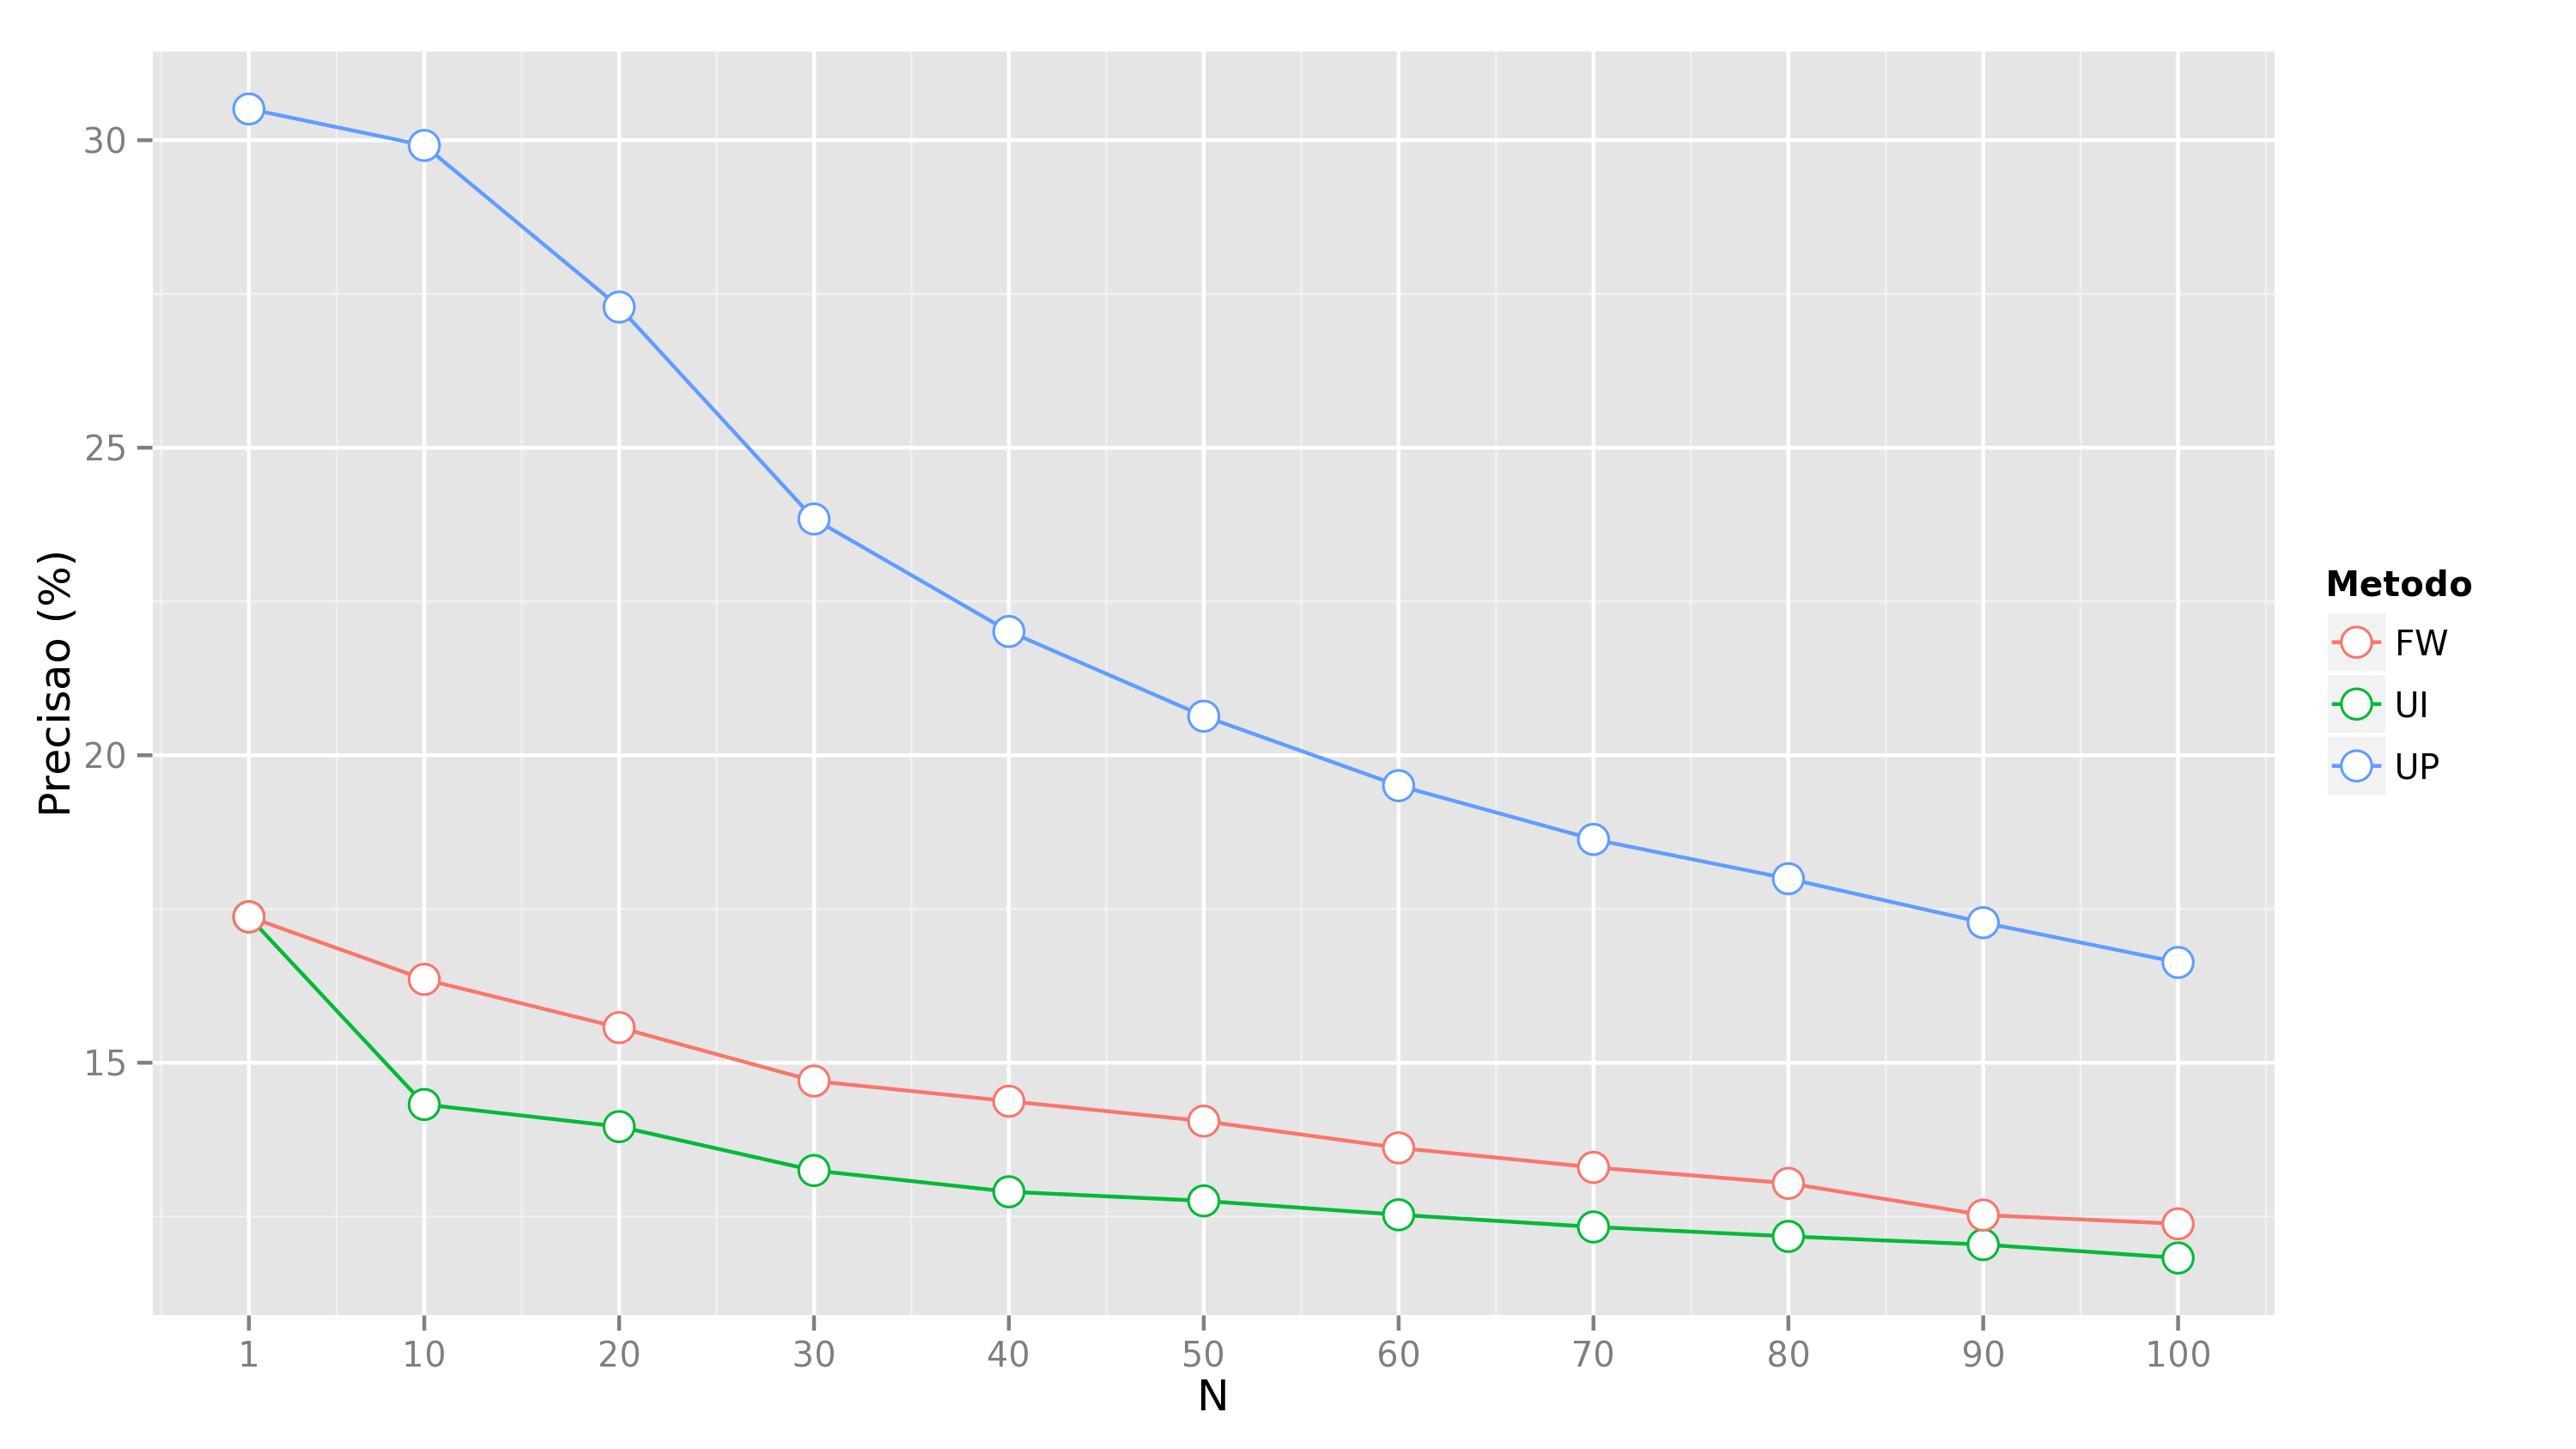
\includegraphics[width=1\textwidth]{img/precision_N}
    \end{center}
    \label{fig:precision_N}
    \caption{Precisão em função do tamanho da lista de recomendações $N$}
\end{figure}


\begin{figure}[htp]
    \begin{center}
    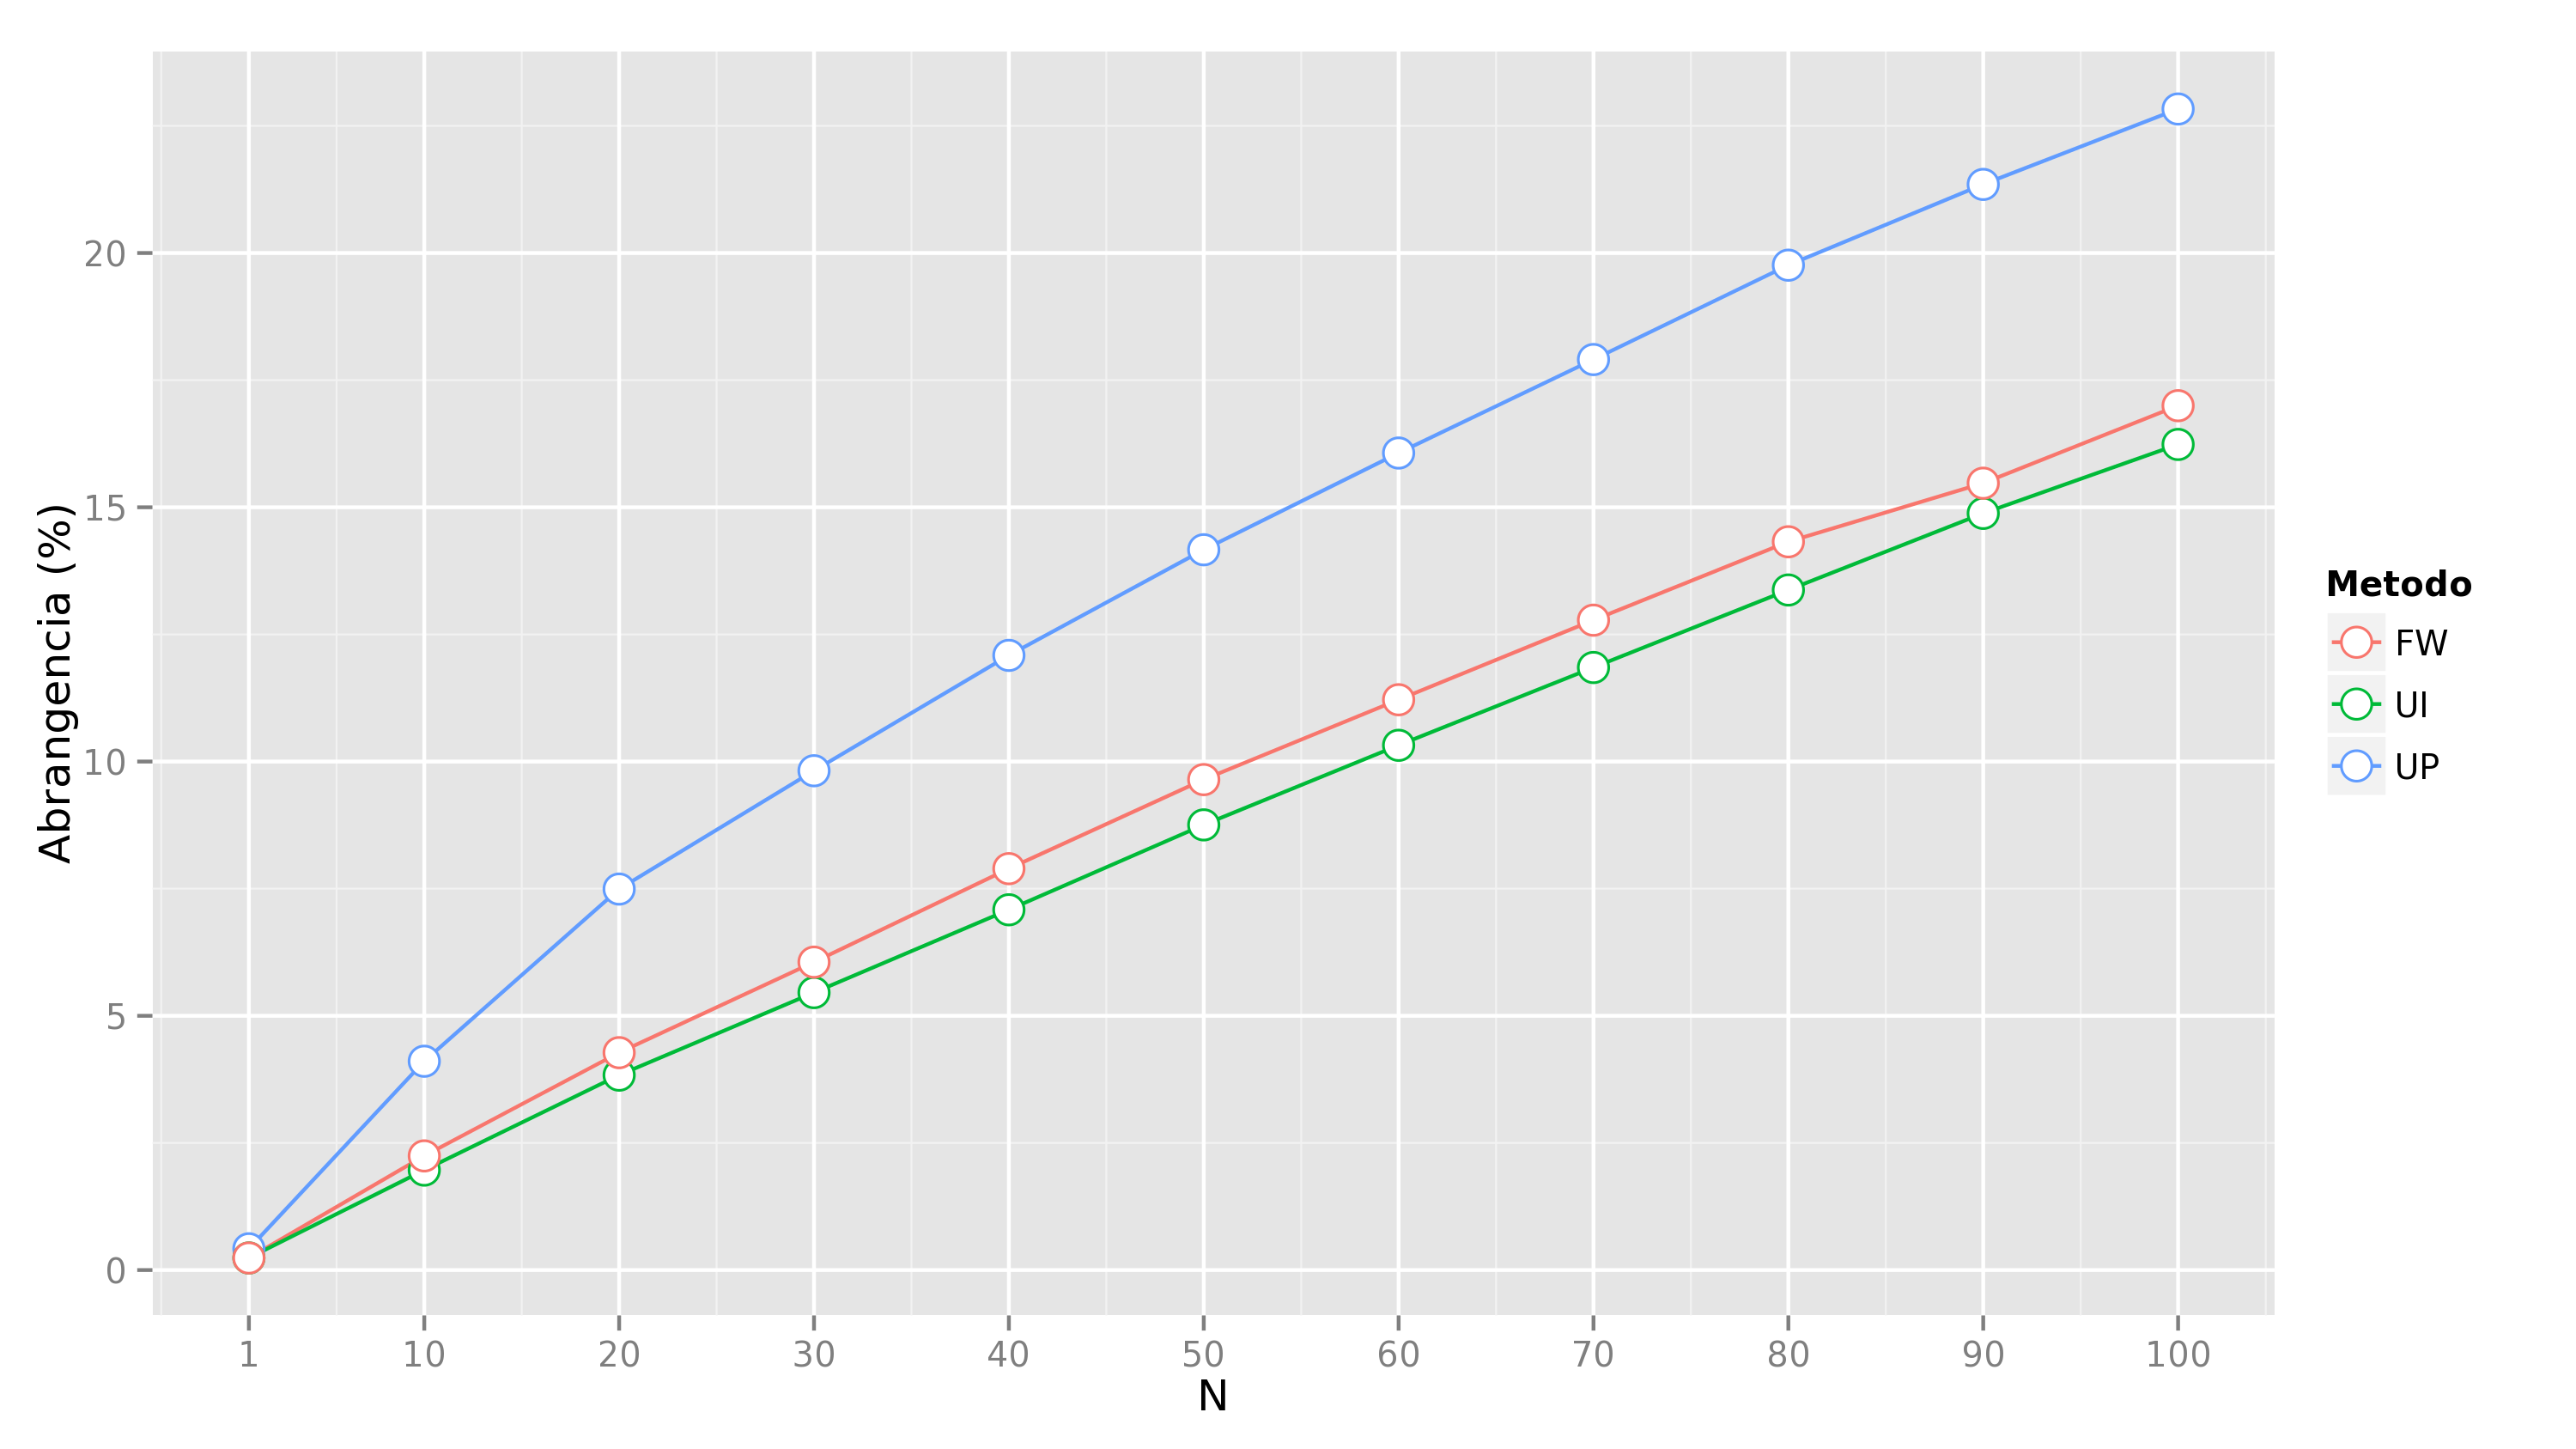
\includegraphics[width=1\textwidth]{img/recall_N}
    \end{center}
    \label{fig:recall_N}
    \caption{Abrangência em função do tamanho da lista de recomendações $N$}
\end{figure}

\begin{figure}[htp]
    \begin{center}
    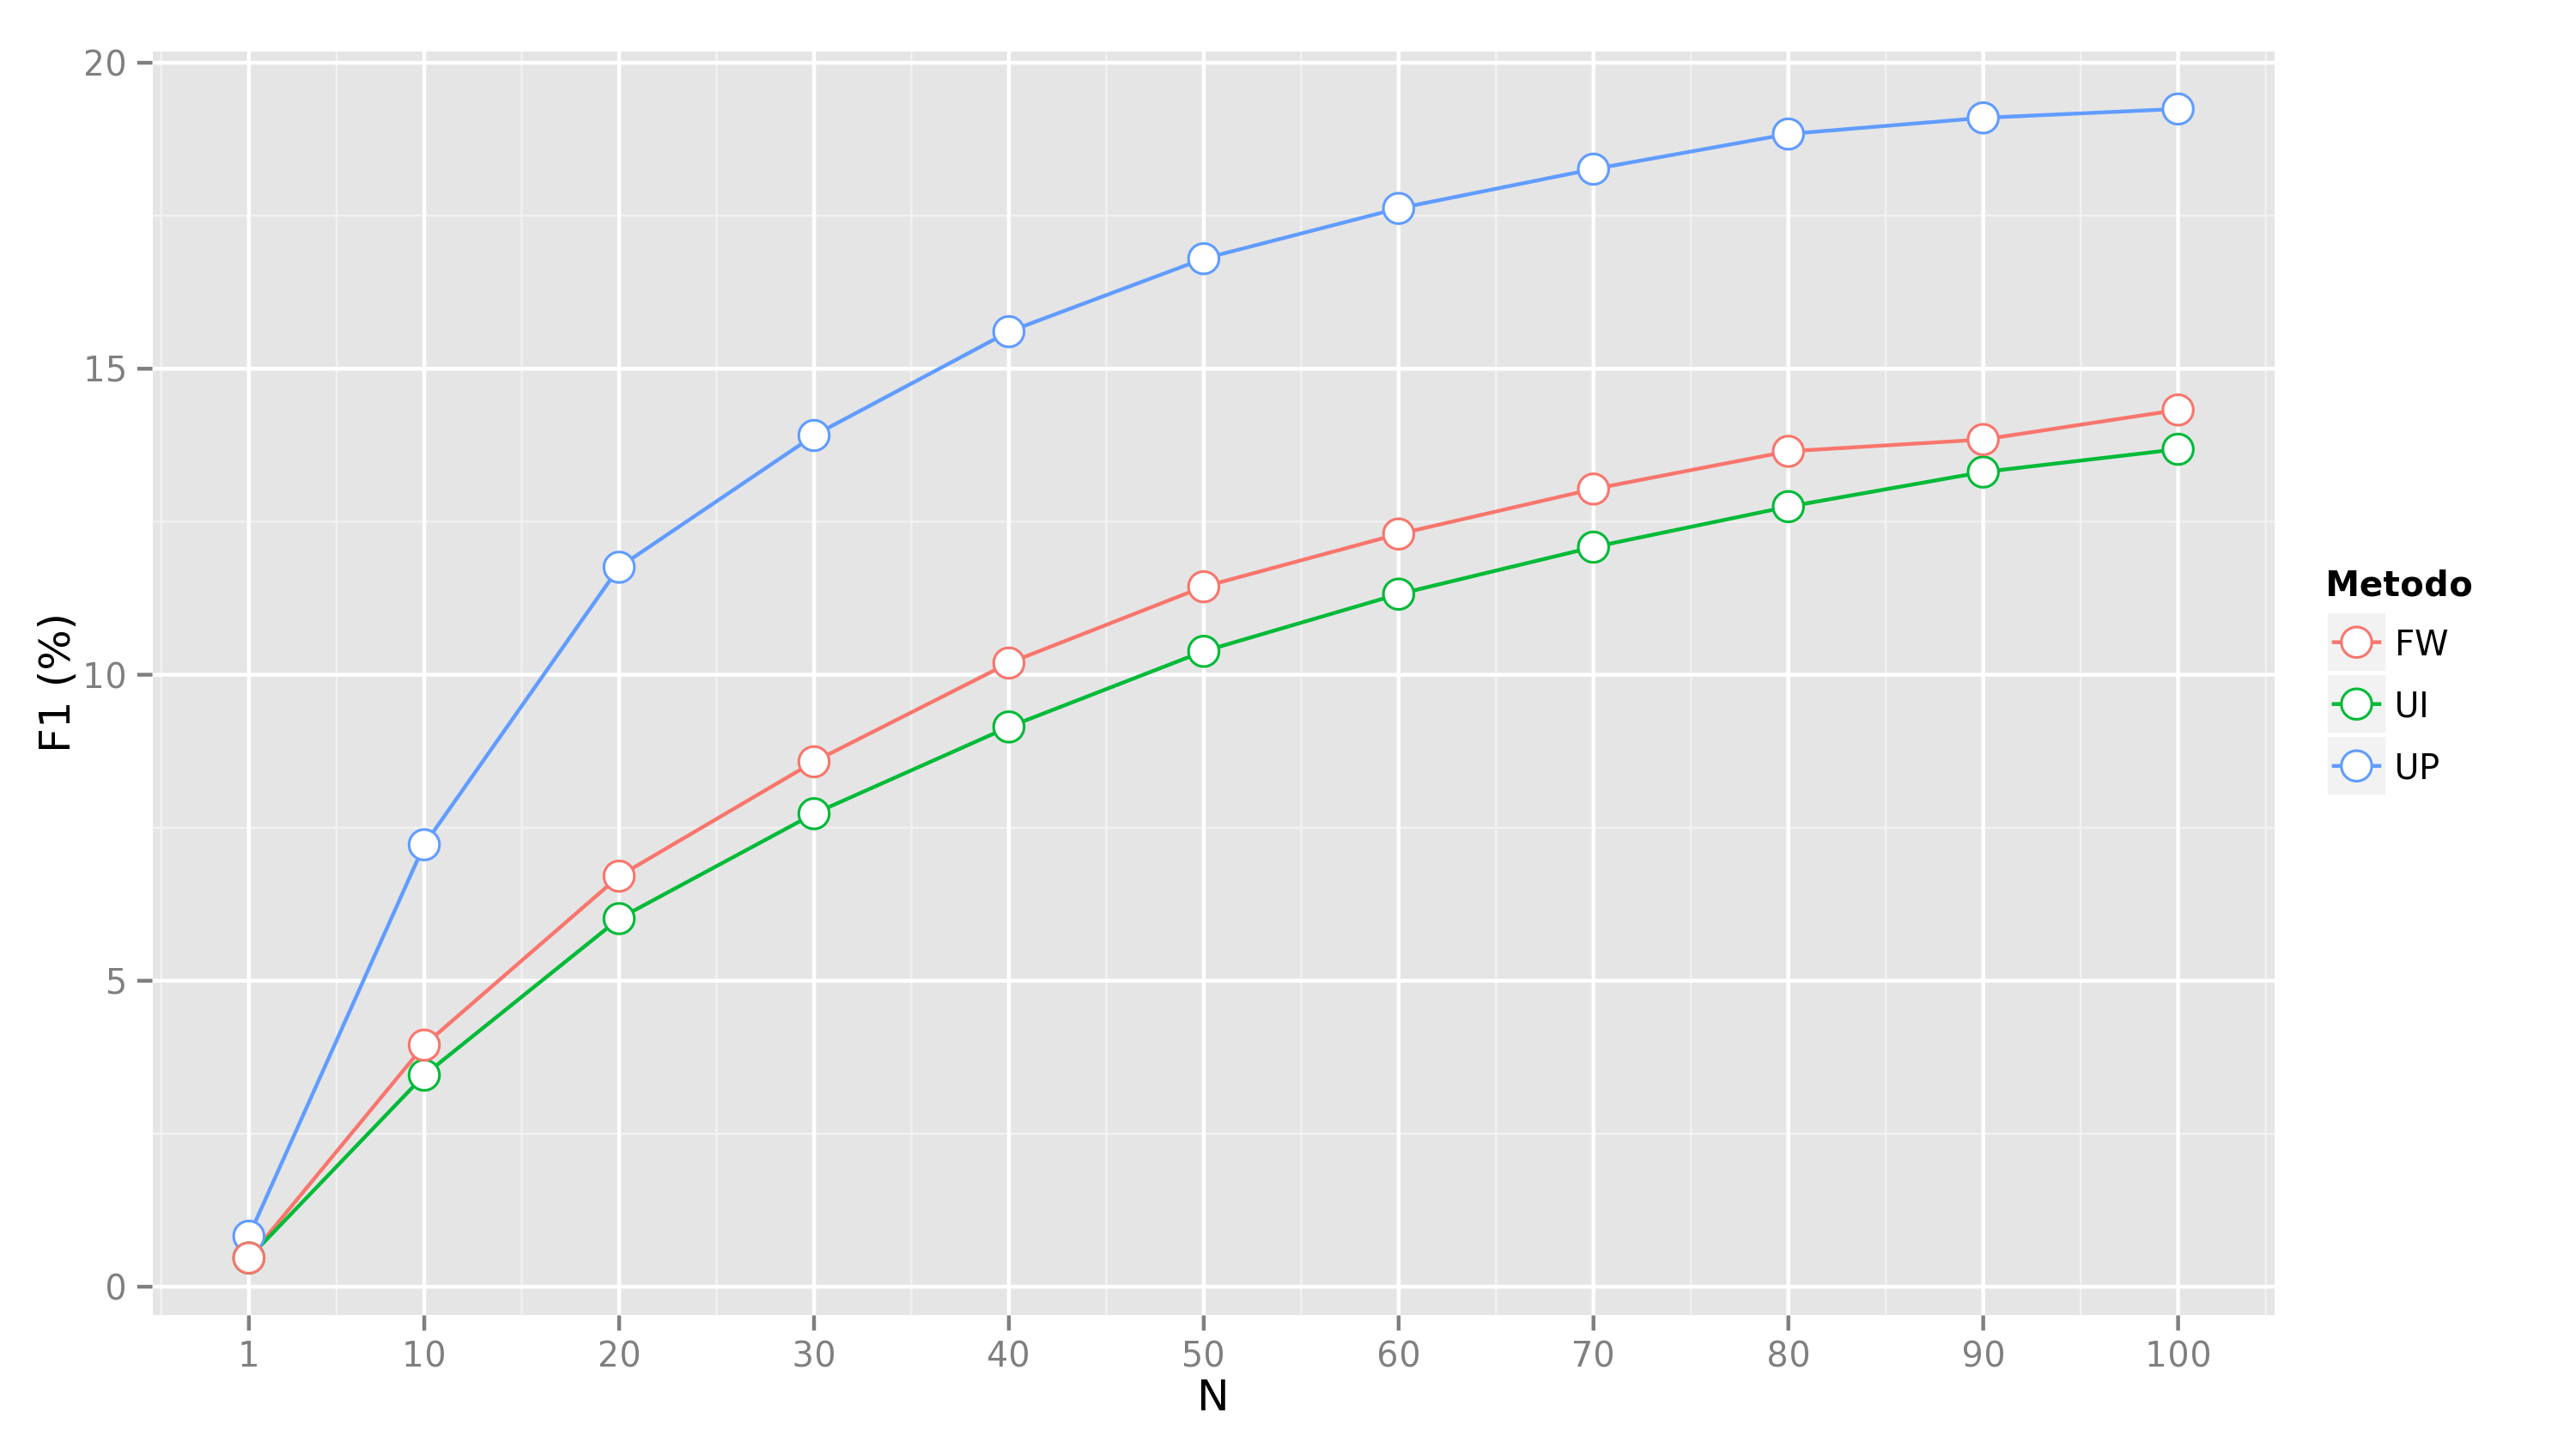
\includegraphics[width=1\textwidth]{img/F1_N}
    \end{center}
    \label{fig:F1_N}
    \caption{Medida $F_1$ em função do tamanho da lista de recomendações $N$}
\end{figure}

\begin{figure}[htp]
    \begin{center}
    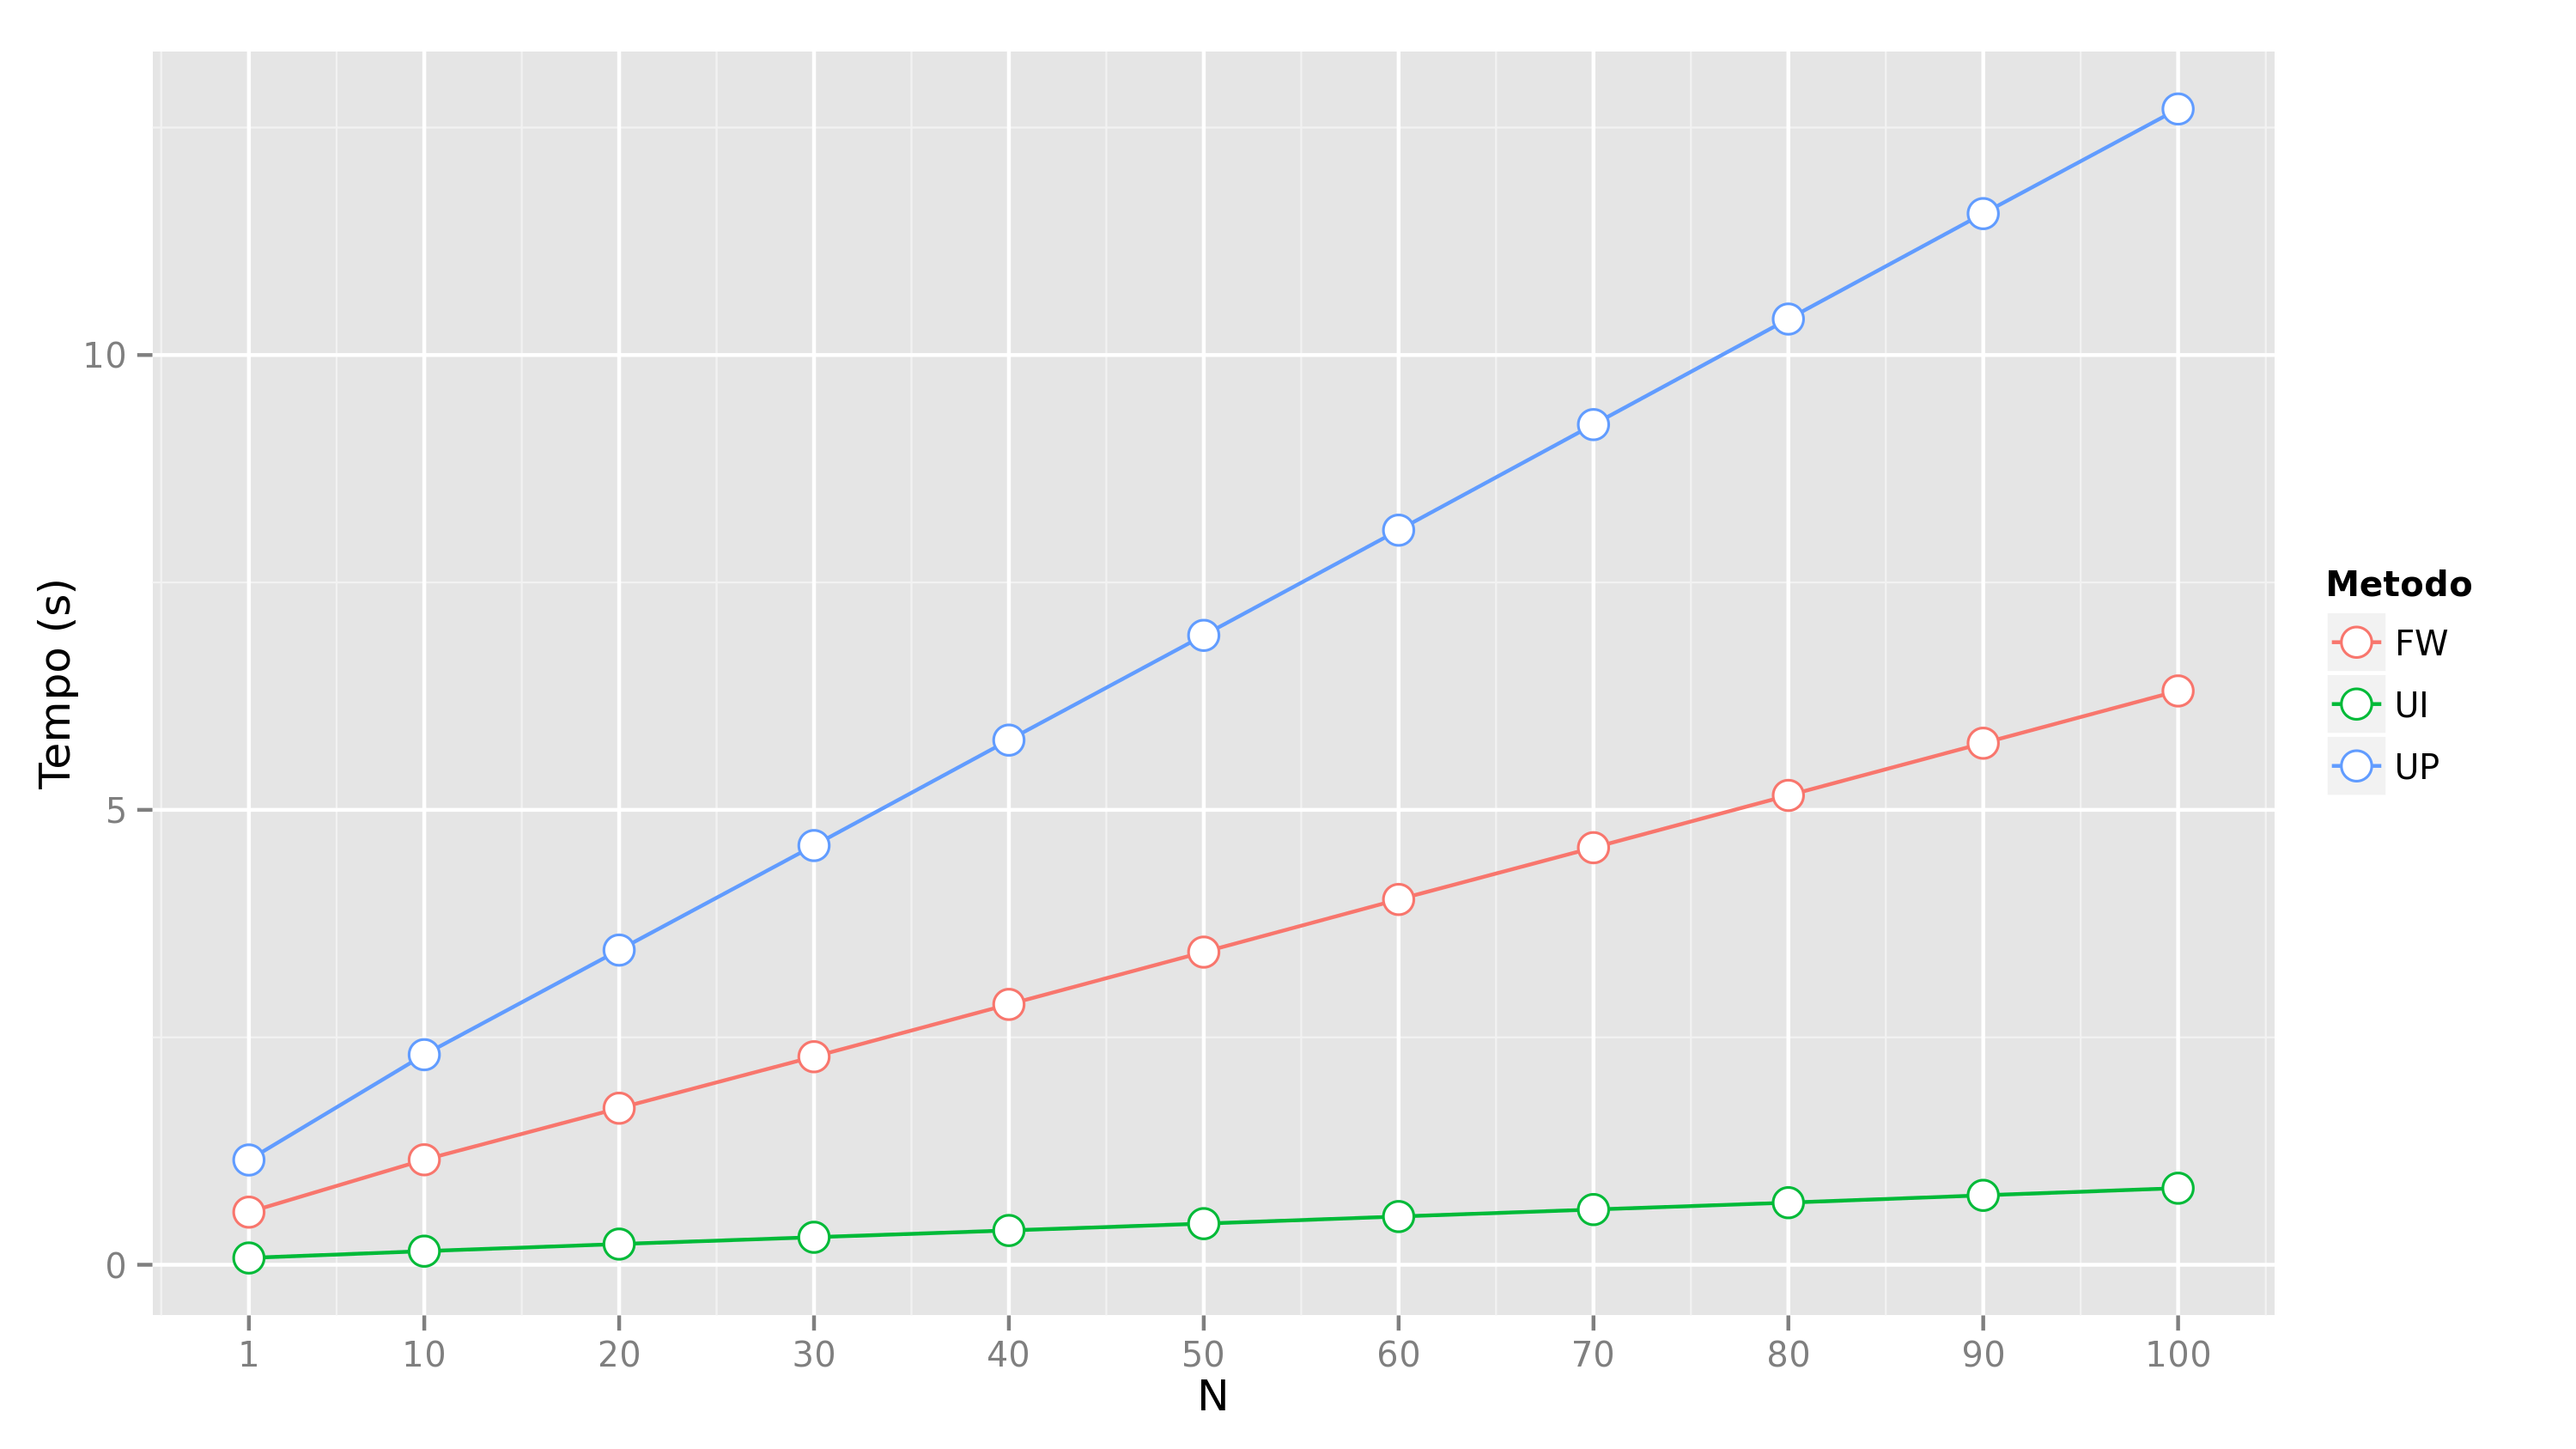
\includegraphics[width=1\textwidth]{img/time_N}
    \end{center}
    \label{fig:time_N}
    \caption{Tempo de execução em função do tamanho da lista de recomendações $N$}
\end{figure}

Contrariamente ao esperado, a qualidade de recomendação do algoritmo UI é sensivelmente inferior à do algoritmo UP. Isso se deve ao fato de a correlação usuário-item daquele método colocar ênfase no valor do atributo $a_{if}$, mesmo que esses atributos não sejam diretamente proporcionais à preferência do usuário. Esse cálculo é incoerente, por exemplo, para atributos $f=\mathrm{data}$: mesmo que o usuário tenha um elevado interesse $w_{uf}$ por filmes antigos, o valor de $a_{if}$ não leva em conta se sua preferência é por filmes da década de 1970 ou 1990. Nesse caso, o algoritmo indicaria incorretamente que filmes mais recentes são mais adequados para aquele usuário, porque possuem maior $a_{if}$.

A fim de corrigir essa falha no algoritmo UI, seria necessário, por exemplo, aplicar nos atributos $a_{if}$ uma função $g_f$ que crescesse no mesmo sentido do interesse do usuário por aquela \textit{feature}. Dessa forma, o cálculo $\sum_f w_{uf}~g_f\left(a_{if}\right)$ significaria de fato a similaridade entre o usuário $u$ e o item $i$ medida através de seu interesse $g\left(a_{if}\right)$ pelas \textit{features} $f$.

Apesar de alta qualidade das recomendações do método UP, este possui também a maior complexidade computacional. Seu tempo de execução é 2 vezes maior que o do método FW e 4 vezes maior que o do método UI. Todavia, nenhum desses tempos de execução é crítico, tendo em vista que o sistema não seria colocado diretamente à disposição dos clientes, mas que as recomendações seriam enviadas via email, por exemplo. 

Apenas o método UI atende ao requisito de \textit{throughput} mínimo de 28 recomendações para cada usuário por segundo. Dado que a base de testes possui $25\%$ do total de usuários, correspondente a 236 clientes para o banco 100k, o tempo de execução máximo dos métodos deveria ser de $0.15$ min. A fim de melhorar a velocidade das recomendações, a solução mais eficiente é a mudança da linguagem de programação. O uso de linguagens C, C++ ou Python pode melhorar o desempenho computacional em até 500 vezes \cite{benchmarkingR}. 

\section{Percentual da base de aprendizado $T$} % (fold)
\label{sec:percentual_da_base_de_aprendizado_}

A medida que o percentual da base de aprendizados aumenta, a precisão de todos os métodos cresce. Essa observação é consequência direta do caráter colaborativo dos algoritmos, já que a qualidade da recomendação

\begin{figure}[htp]
    \begin{center}
    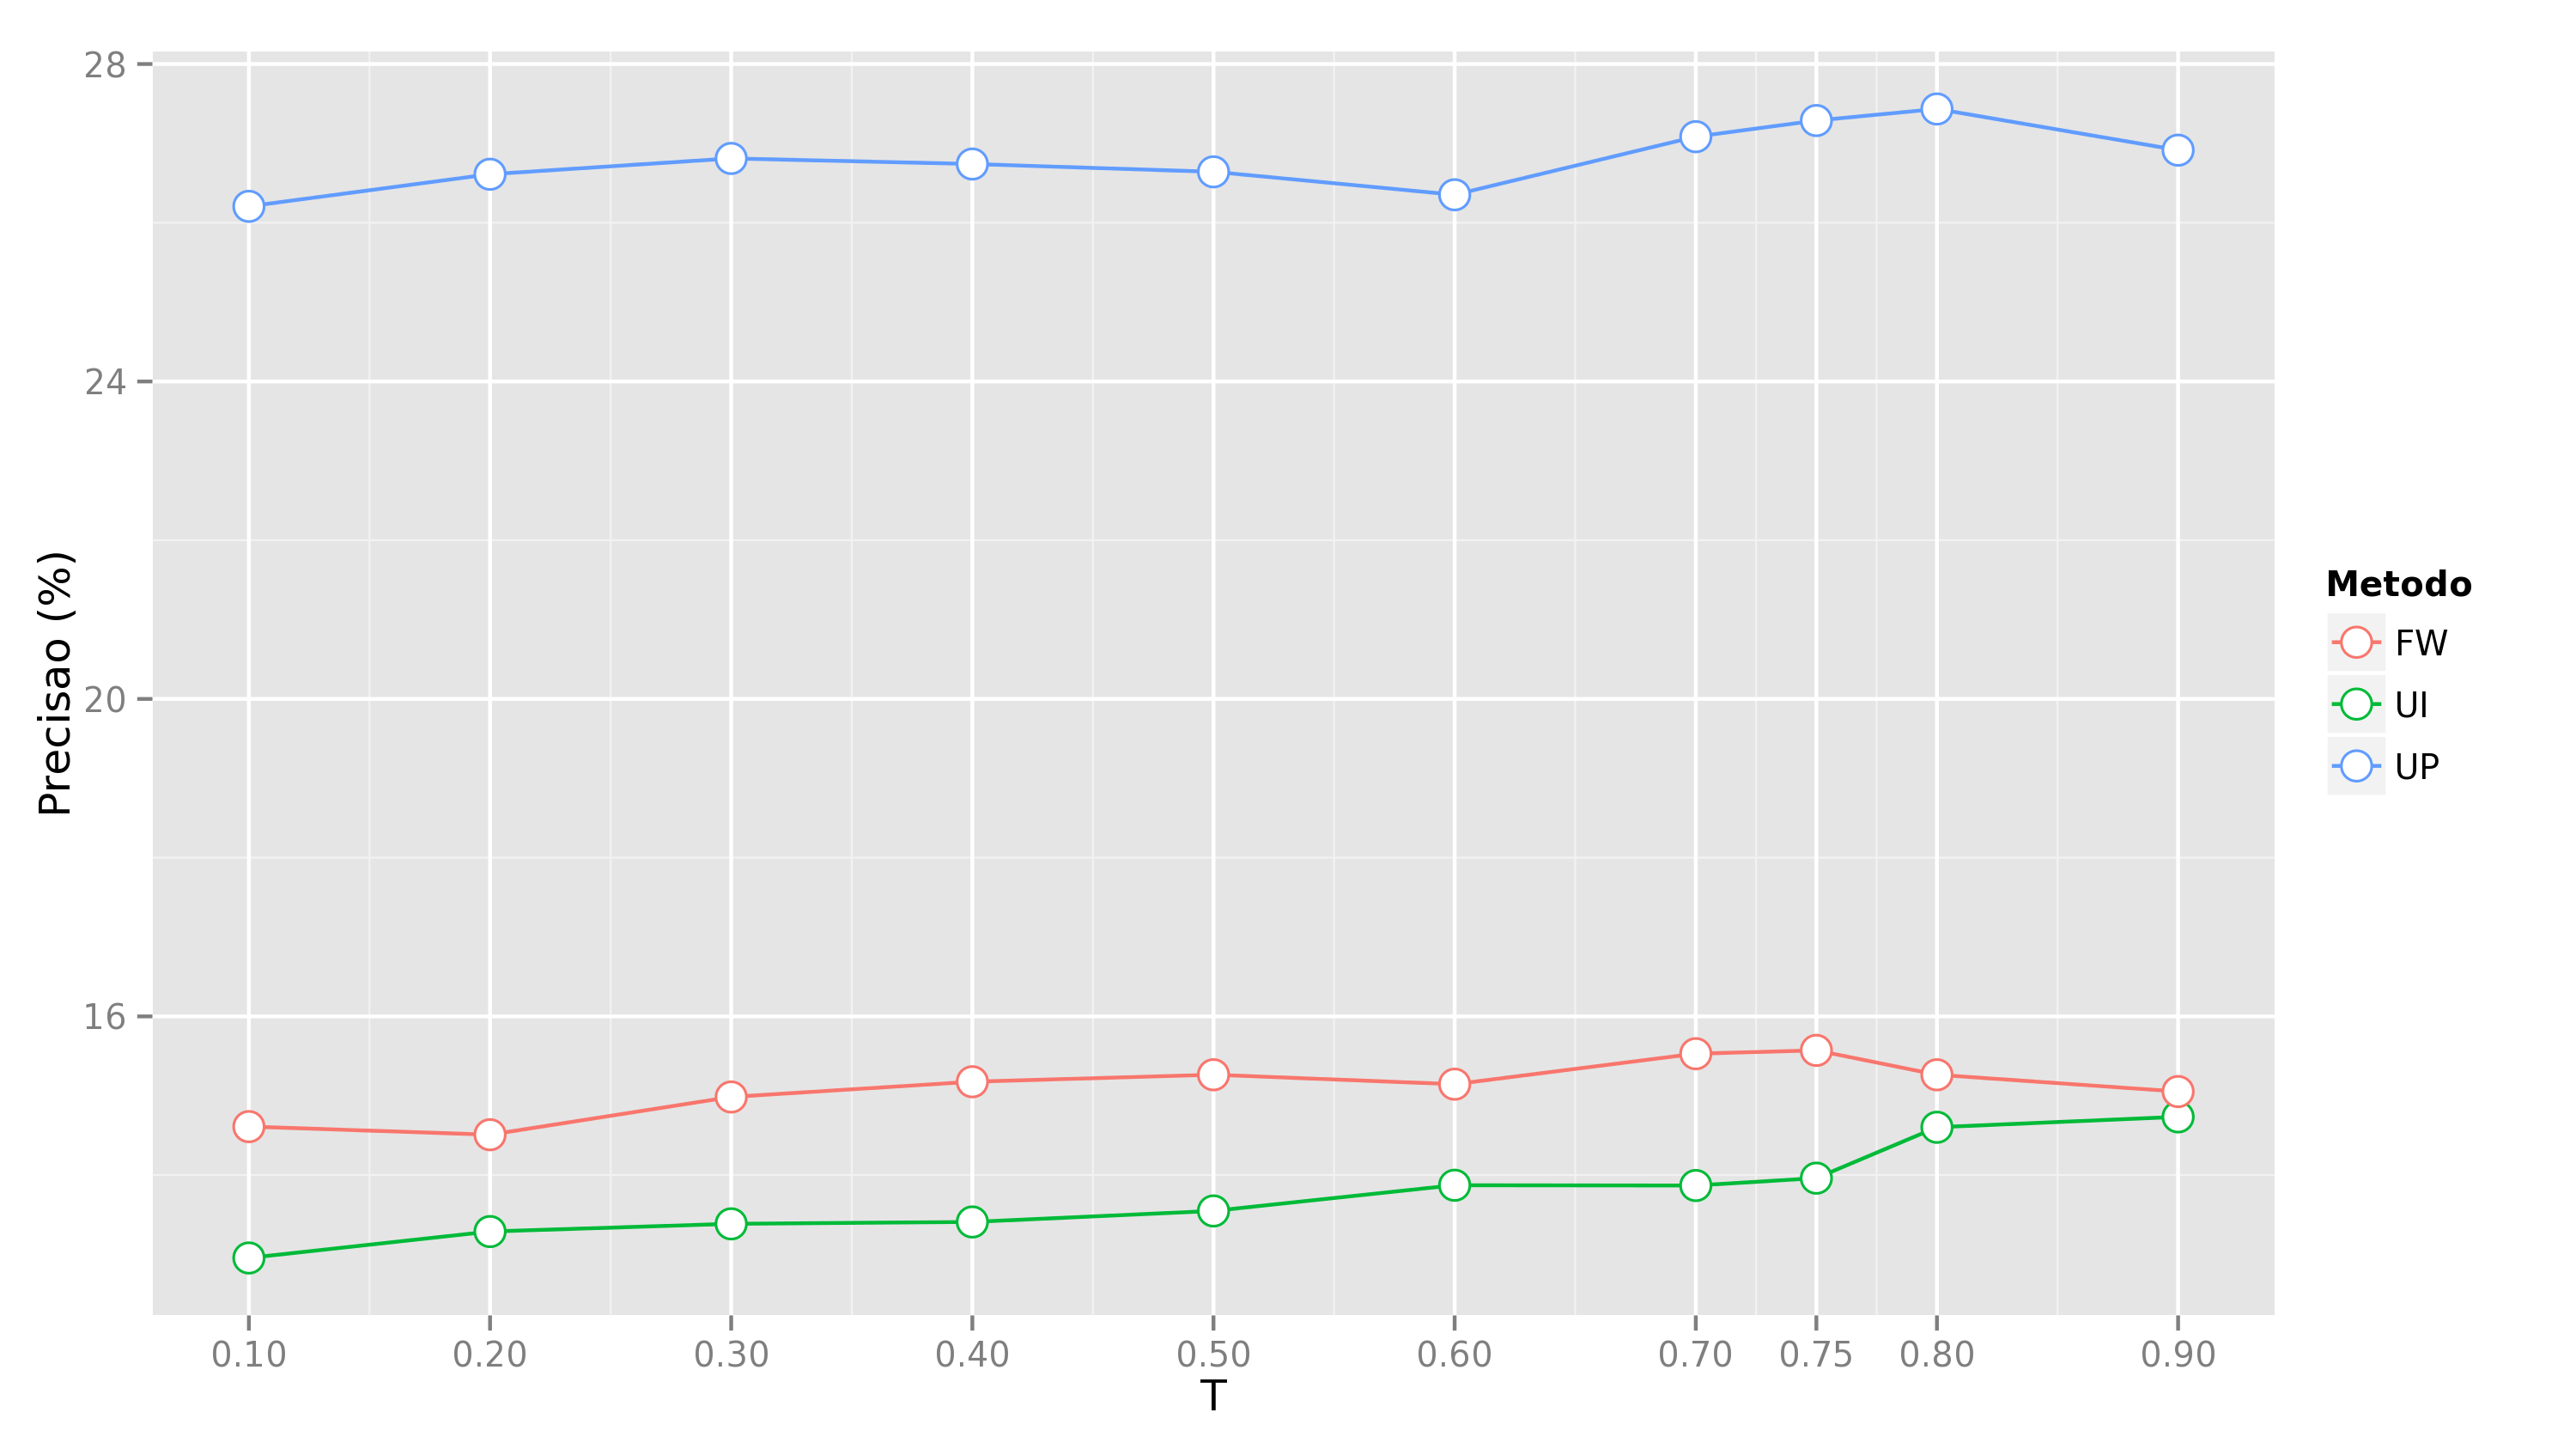
\includegraphics[width=1\textwidth]{img/precision_T}
    \end{center}
    \label{fig:precision_T}
    \caption{Precisão em função do percentual da base de aprendizado $T$}
\end{figure}


\begin{figure}[htp]
    \begin{center}
    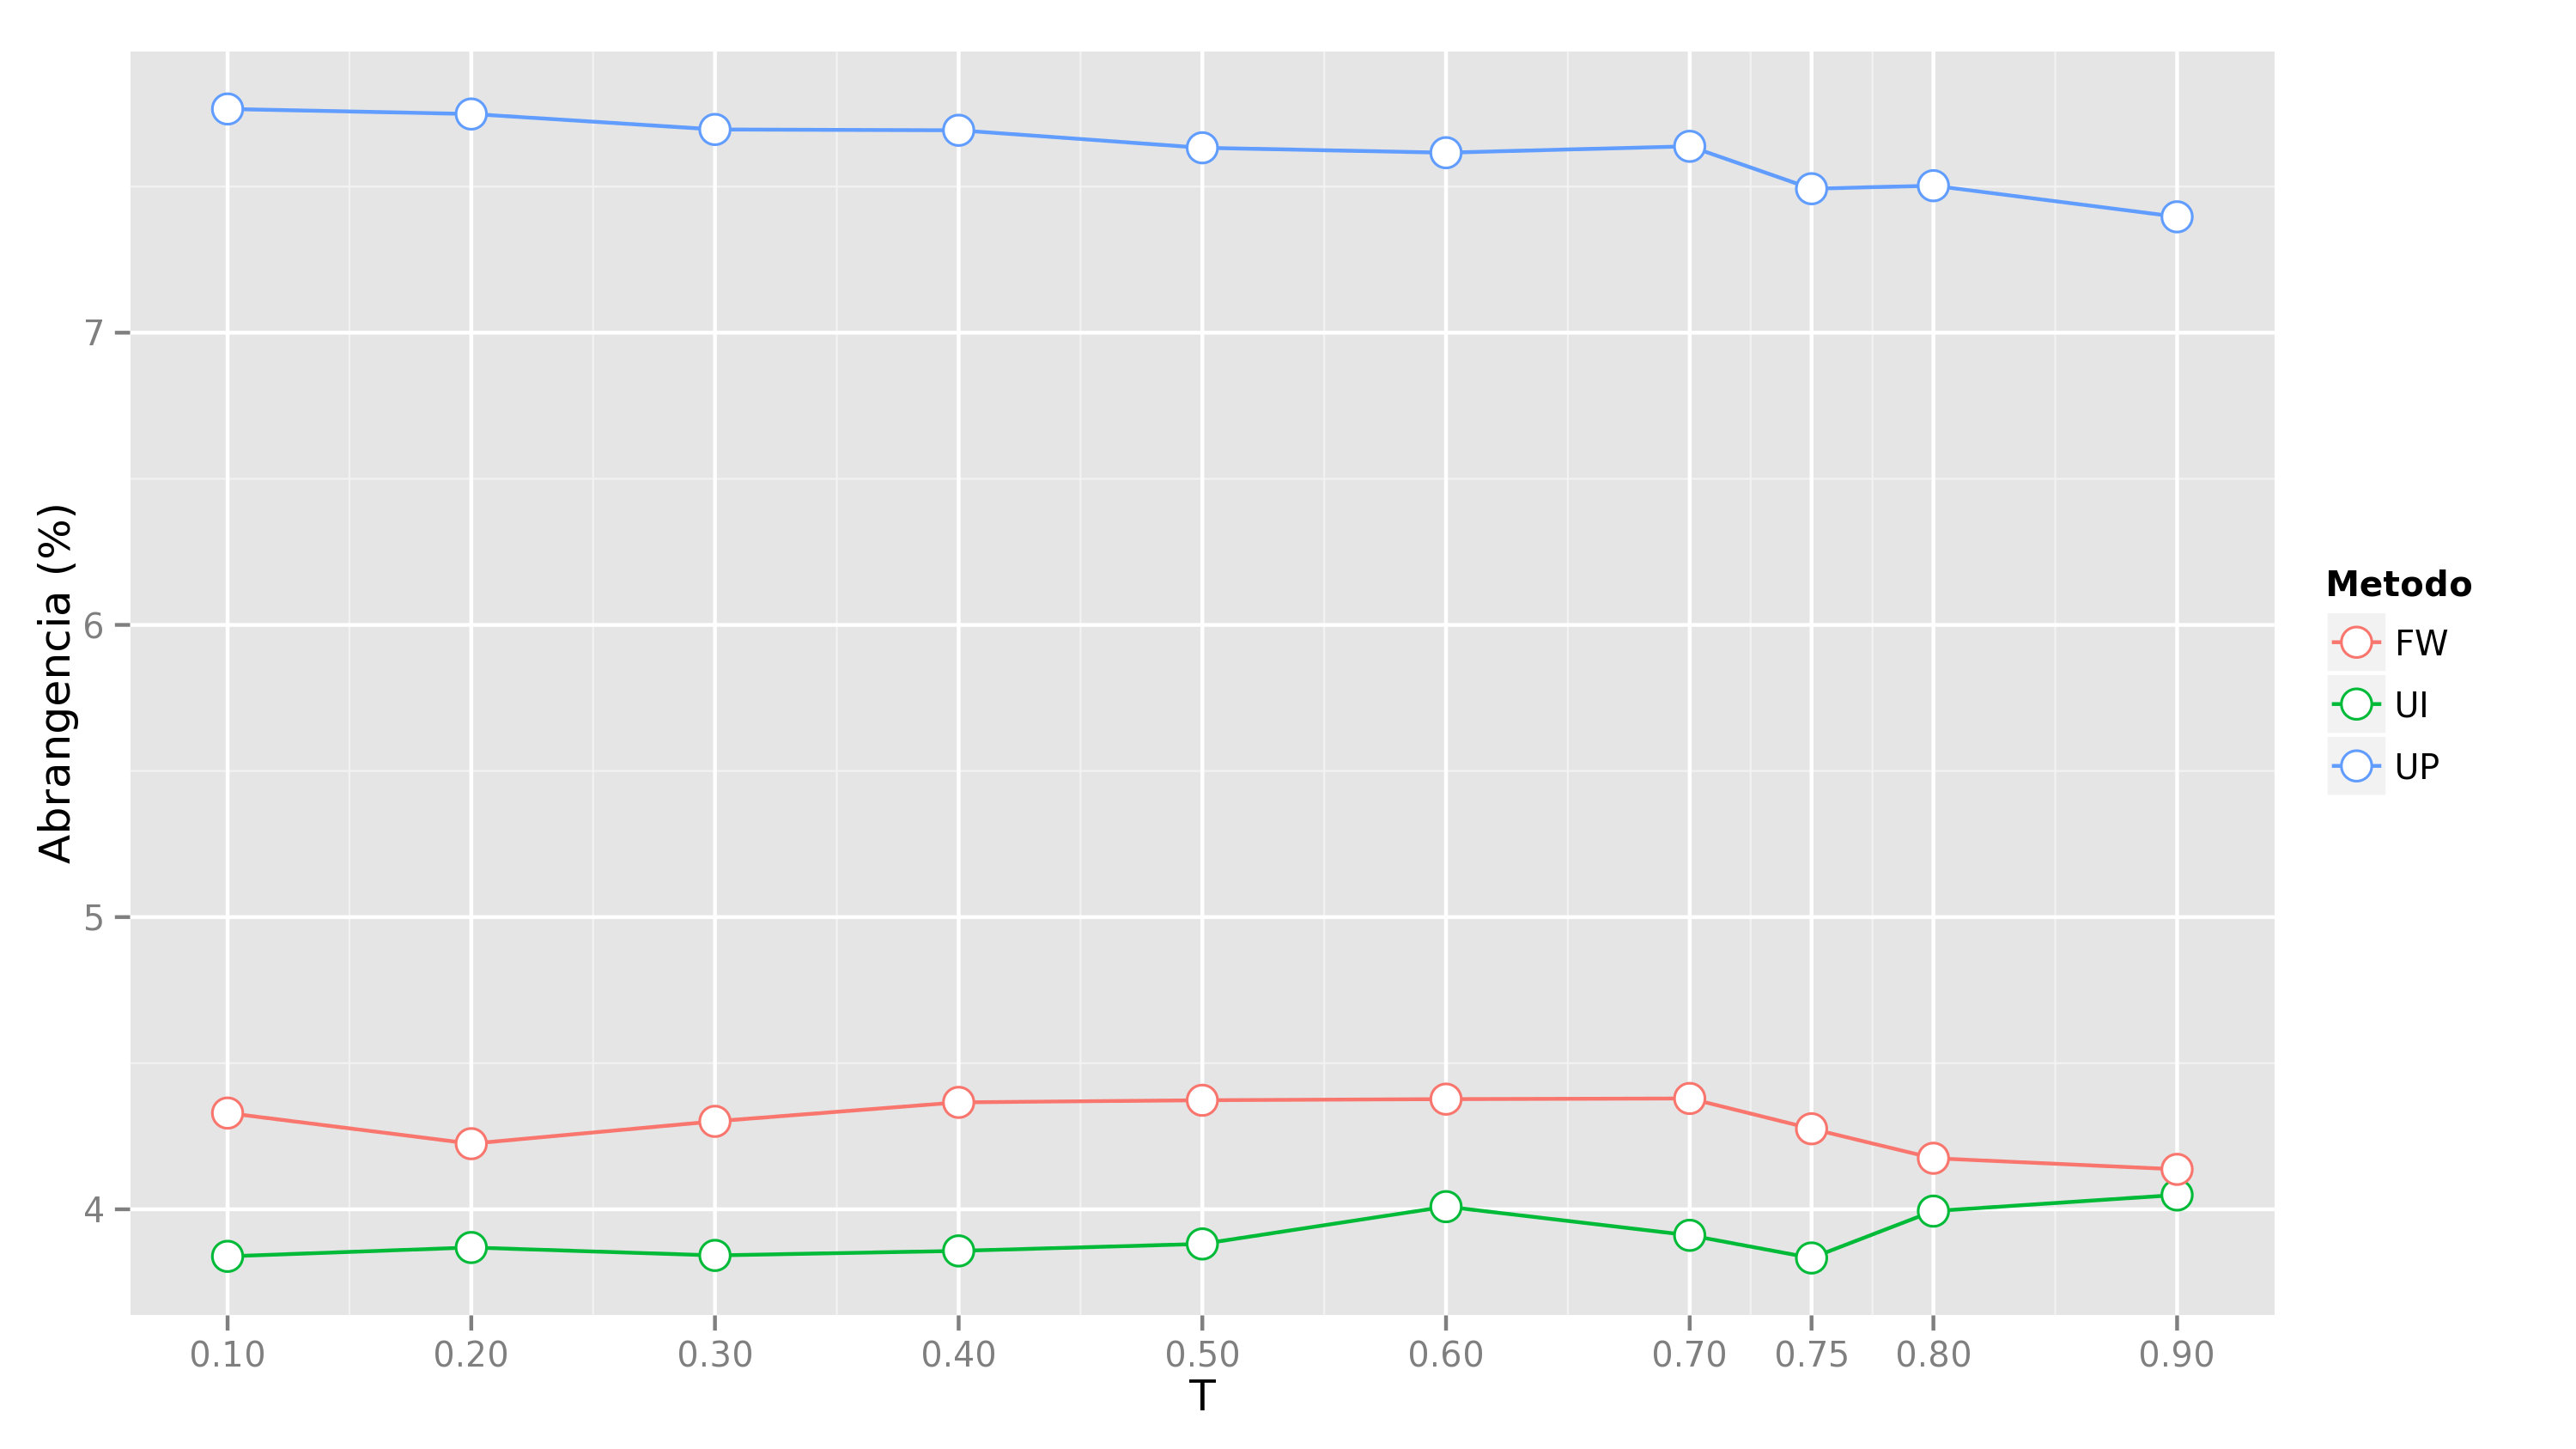
\includegraphics[width=1\textwidth]{img/recall_T}
    \end{center}
    \label{fig:recall_T}
    \caption{Abrangência em função do percentual da base de aprendizado $T$}
\end{figure}

\begin{figure}[htp]
    \begin{center}
    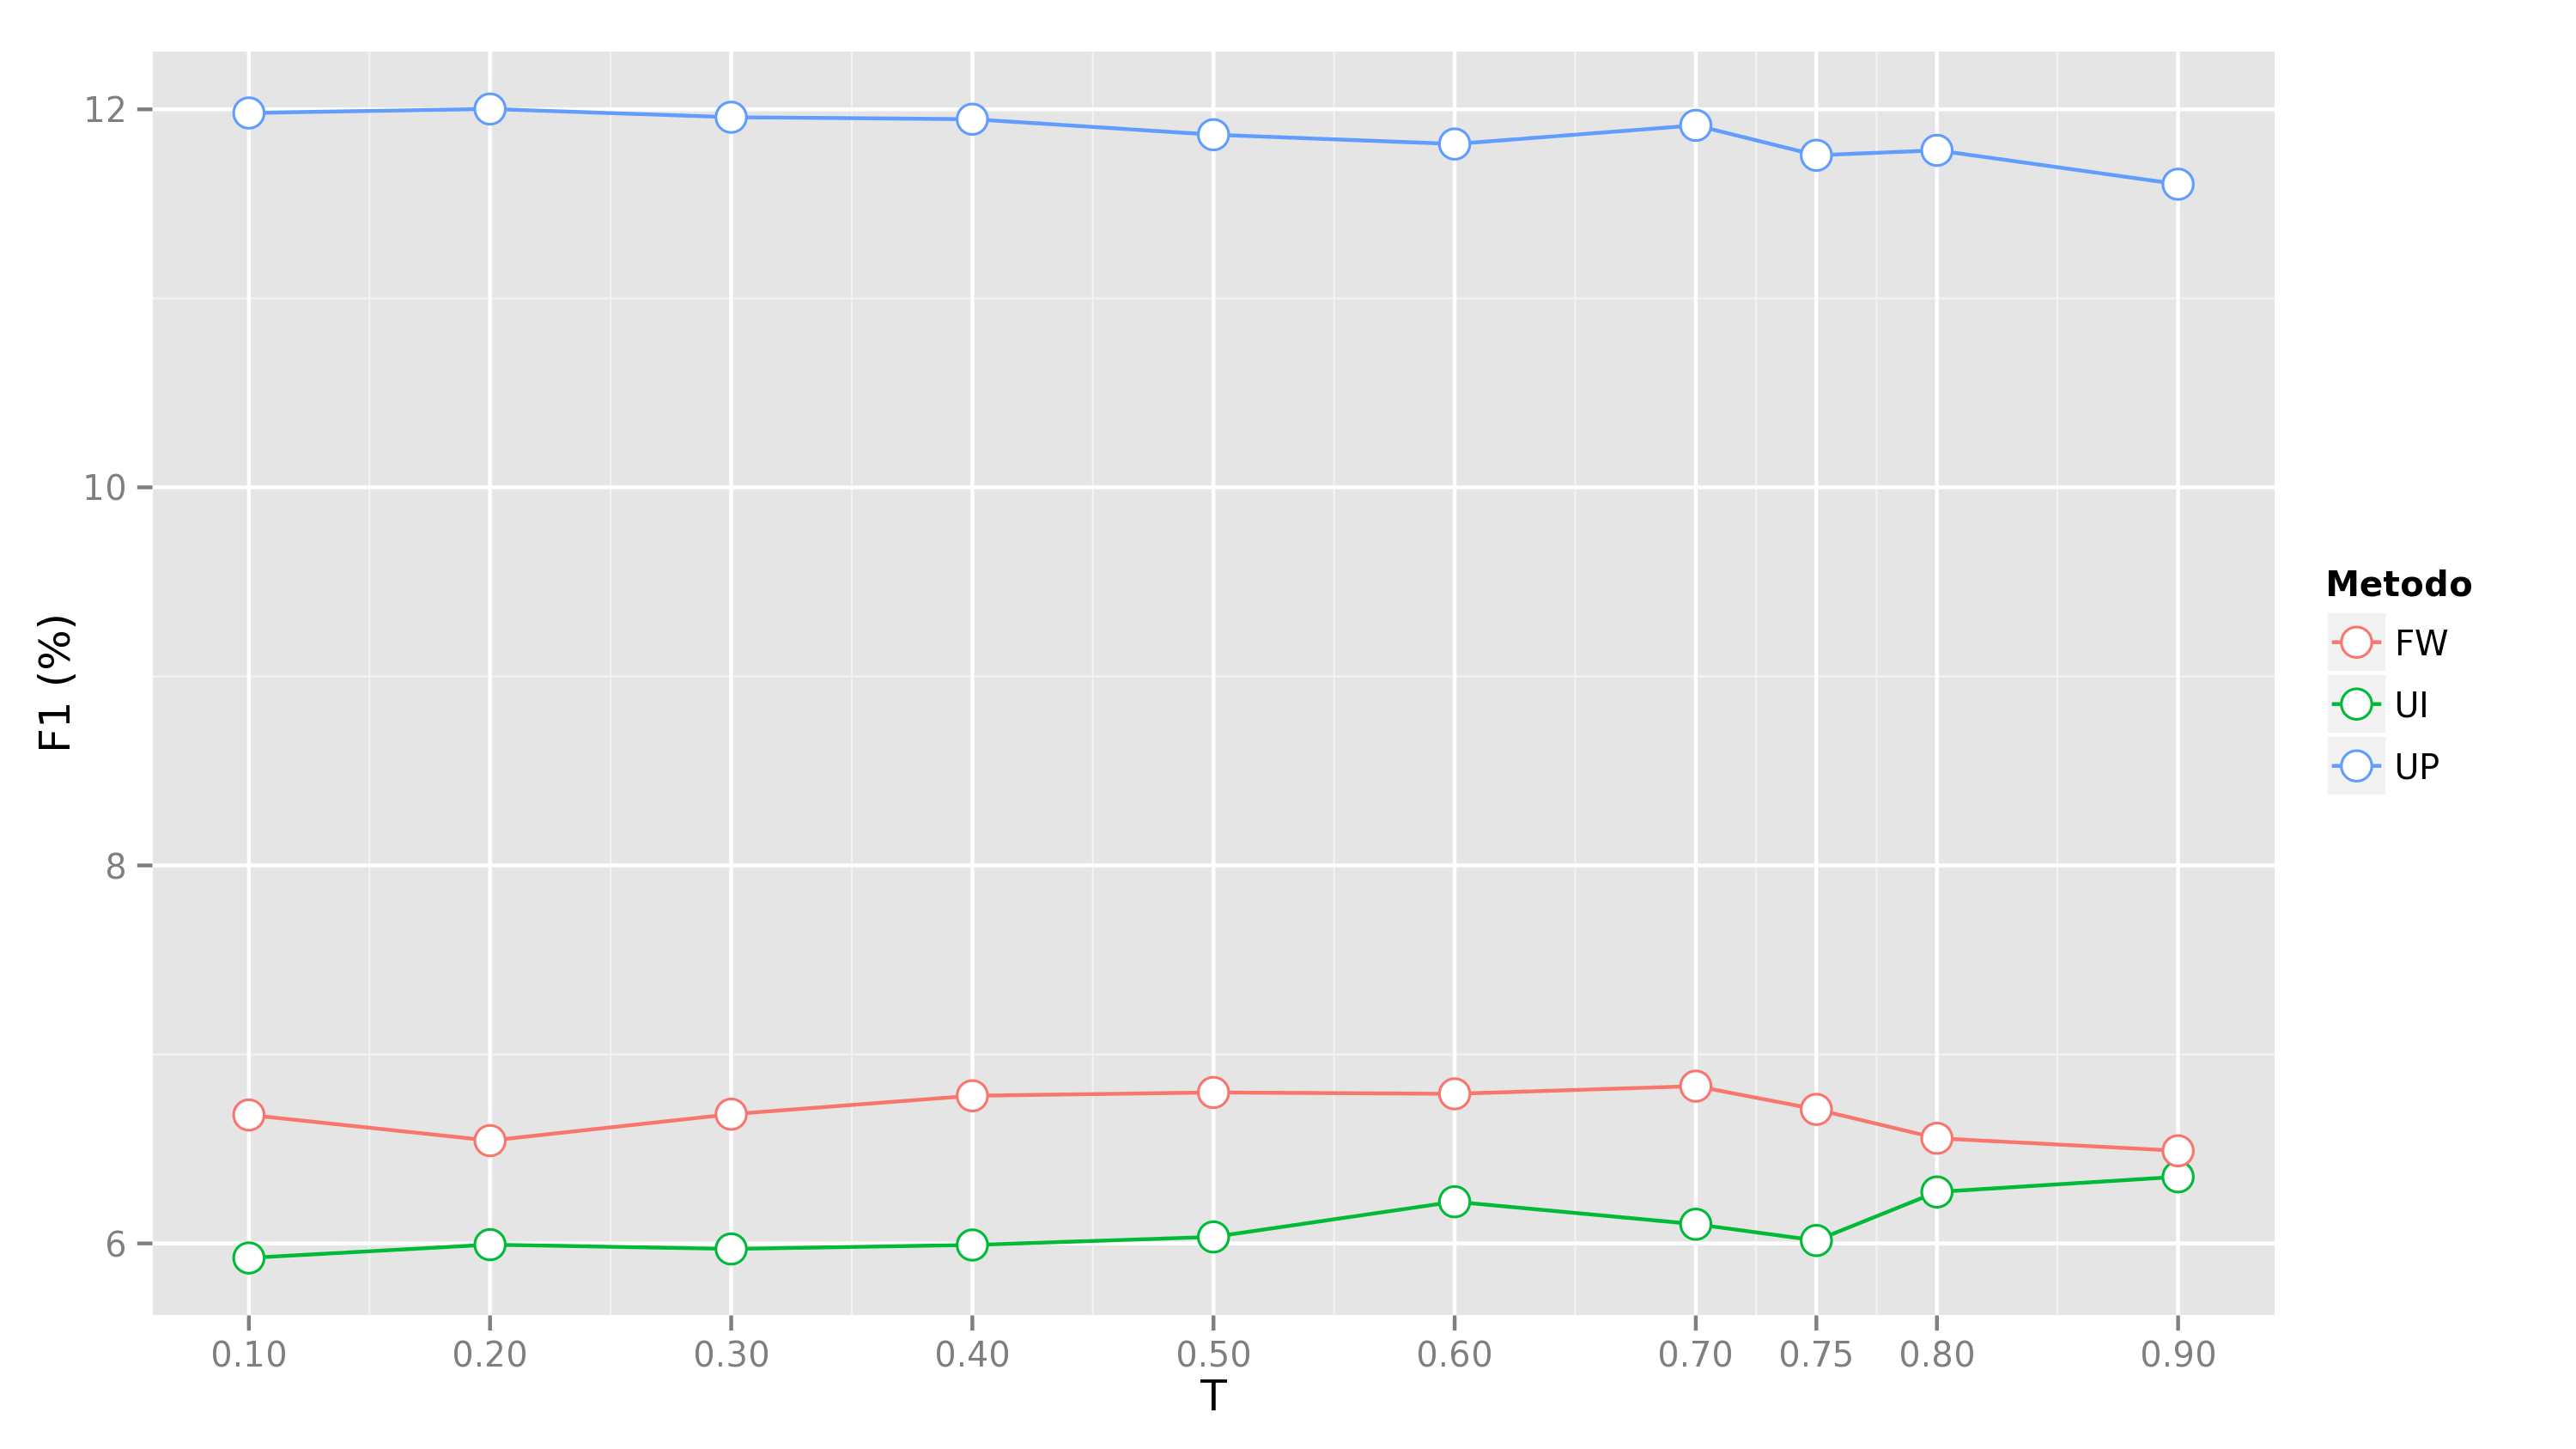
\includegraphics[width=1\textwidth]{img/F1_T}
    \end{center}
    \label{fig:F1_T}
    \caption{Medida $F_1$ em função do percentual da base de aprendizado $T$}
\end{figure}

\begin{figure}[htp]
    \begin{center}
    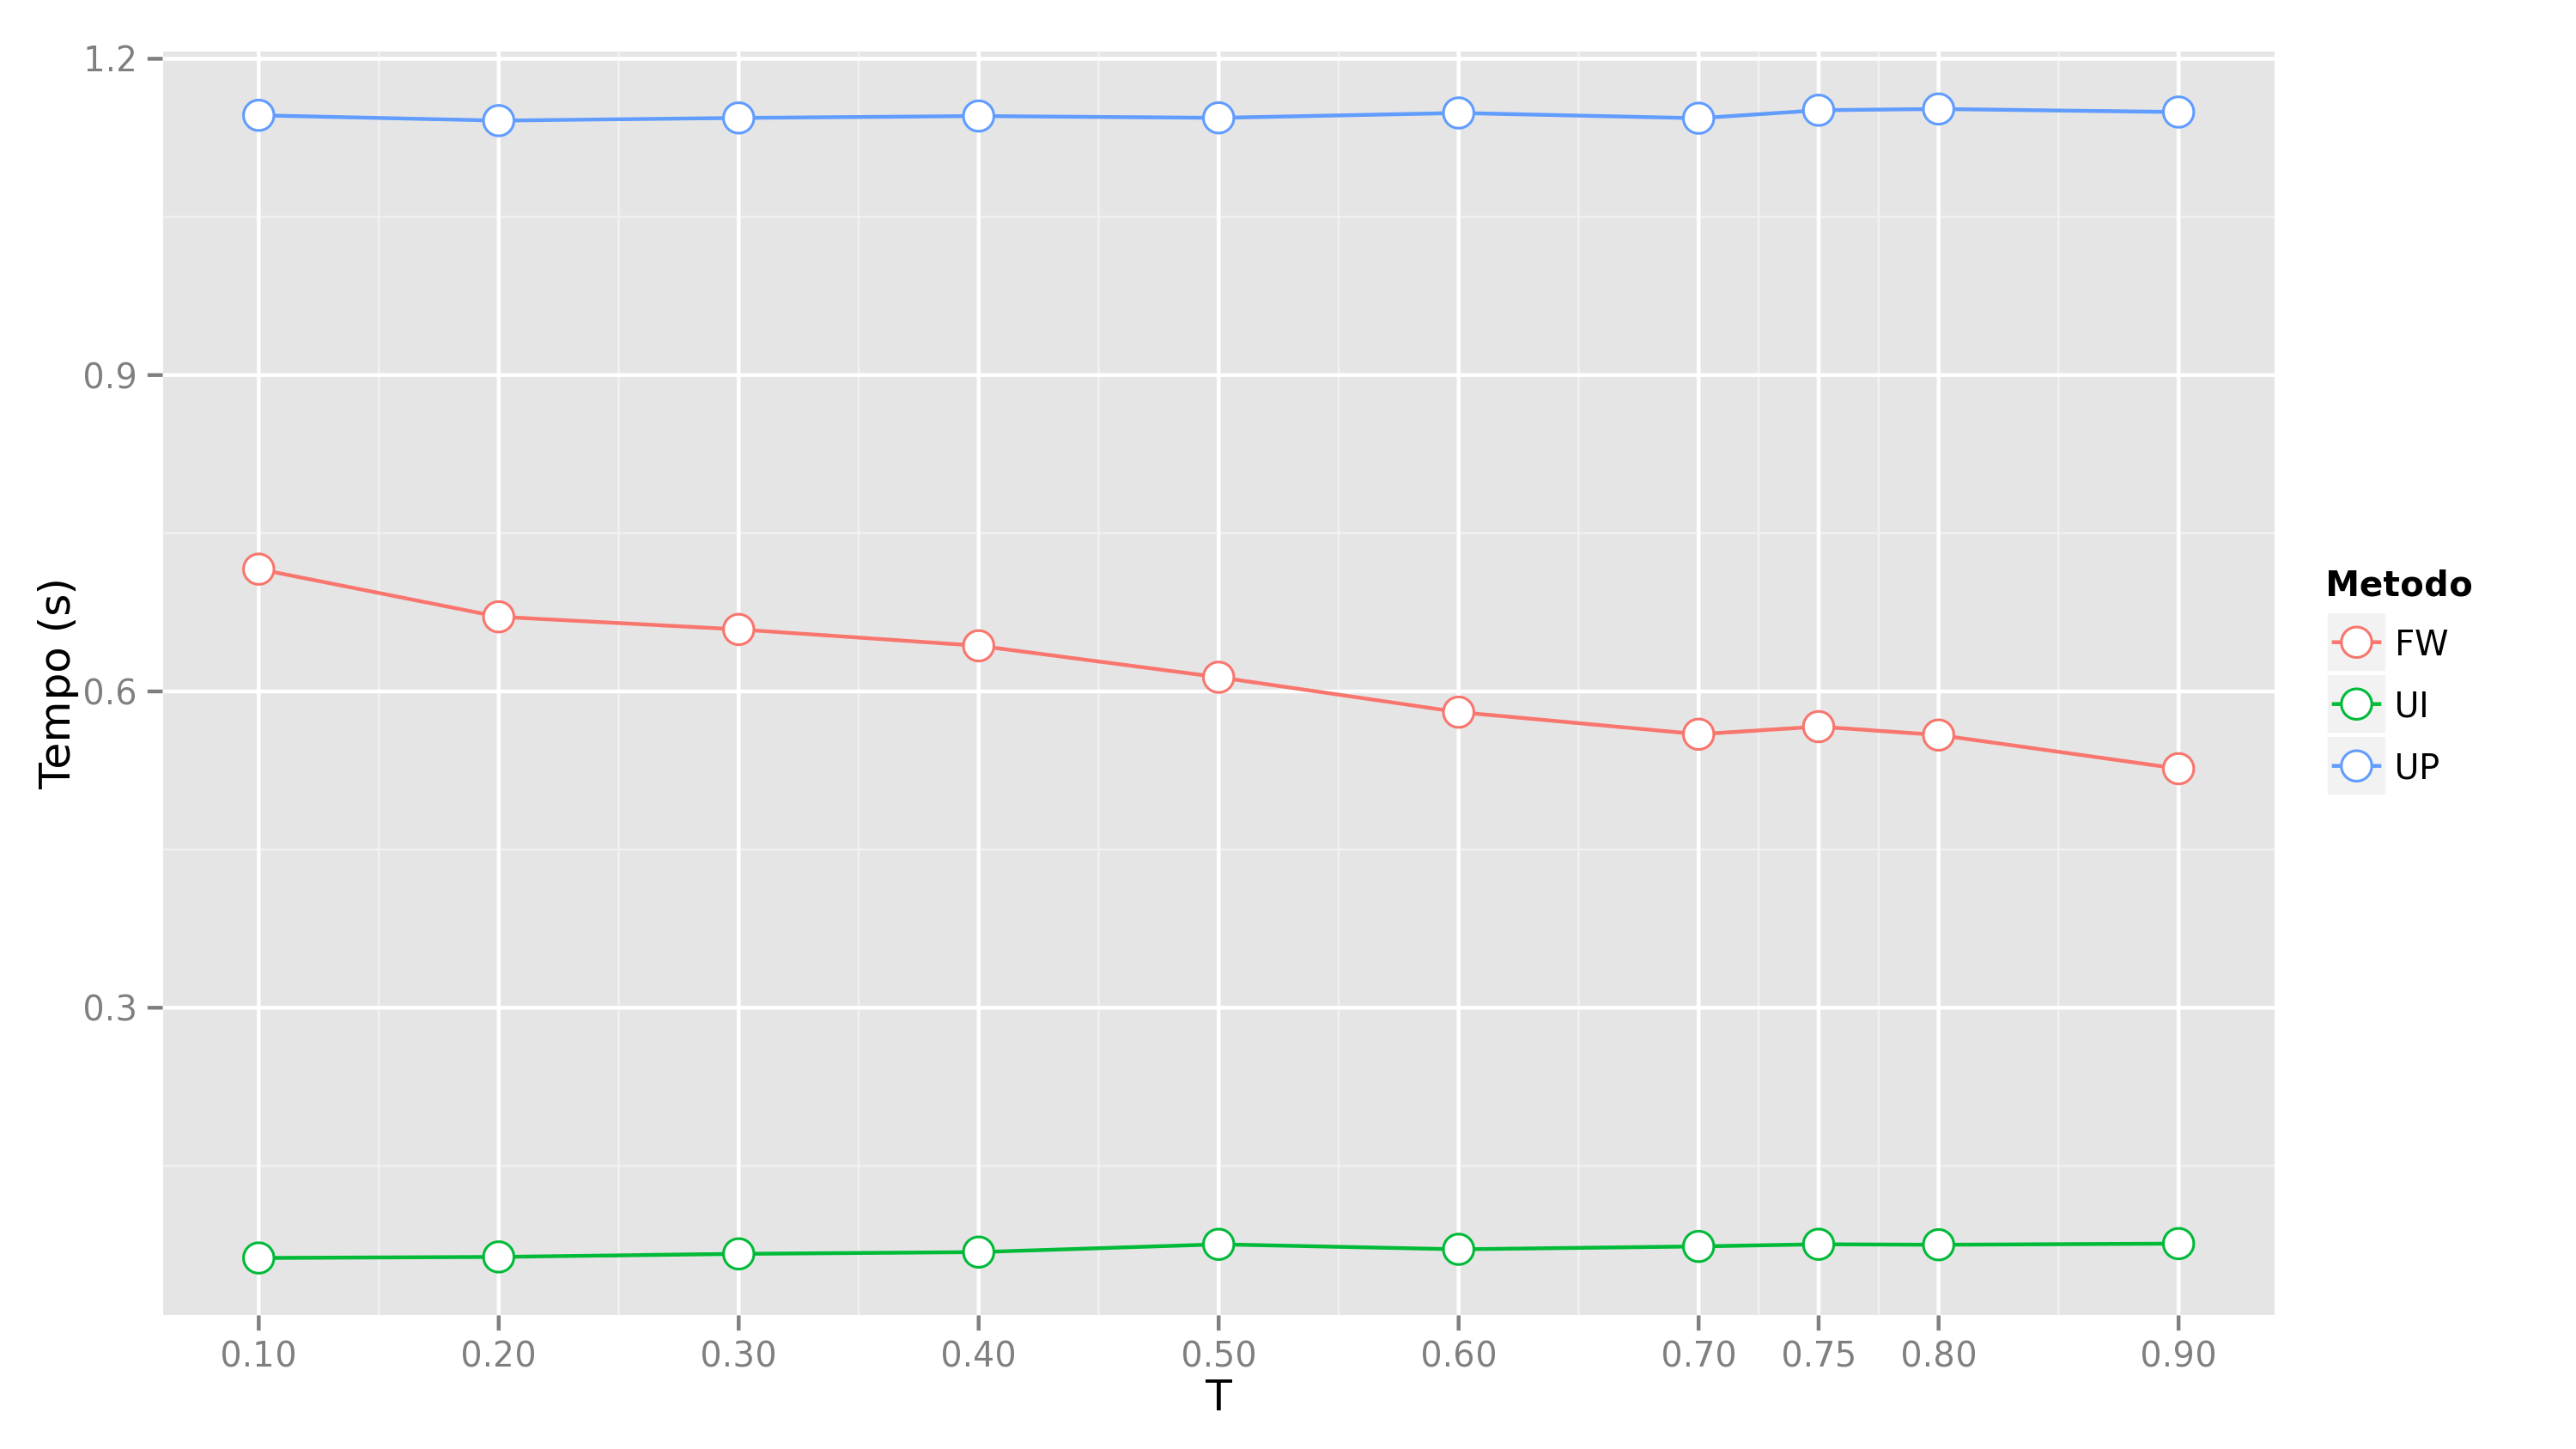
\includegraphics[width=1\textwidth]{img/time_T}
    \end{center}
    \label{fig:time_T}
    \caption{Tempo de execução em função do percentual da base de aprendizado $T$}
\end{figure}


\section{Percentual de avaliações ``escondidas'' dos usuários-teste na validação cruzada $H$} % (fold)
\label{sec:percentual_de_avalia_es_dos_usu_rios_teste_na_valida_o_cruzada}


\begin{figure}[htp]
    \begin{center}
    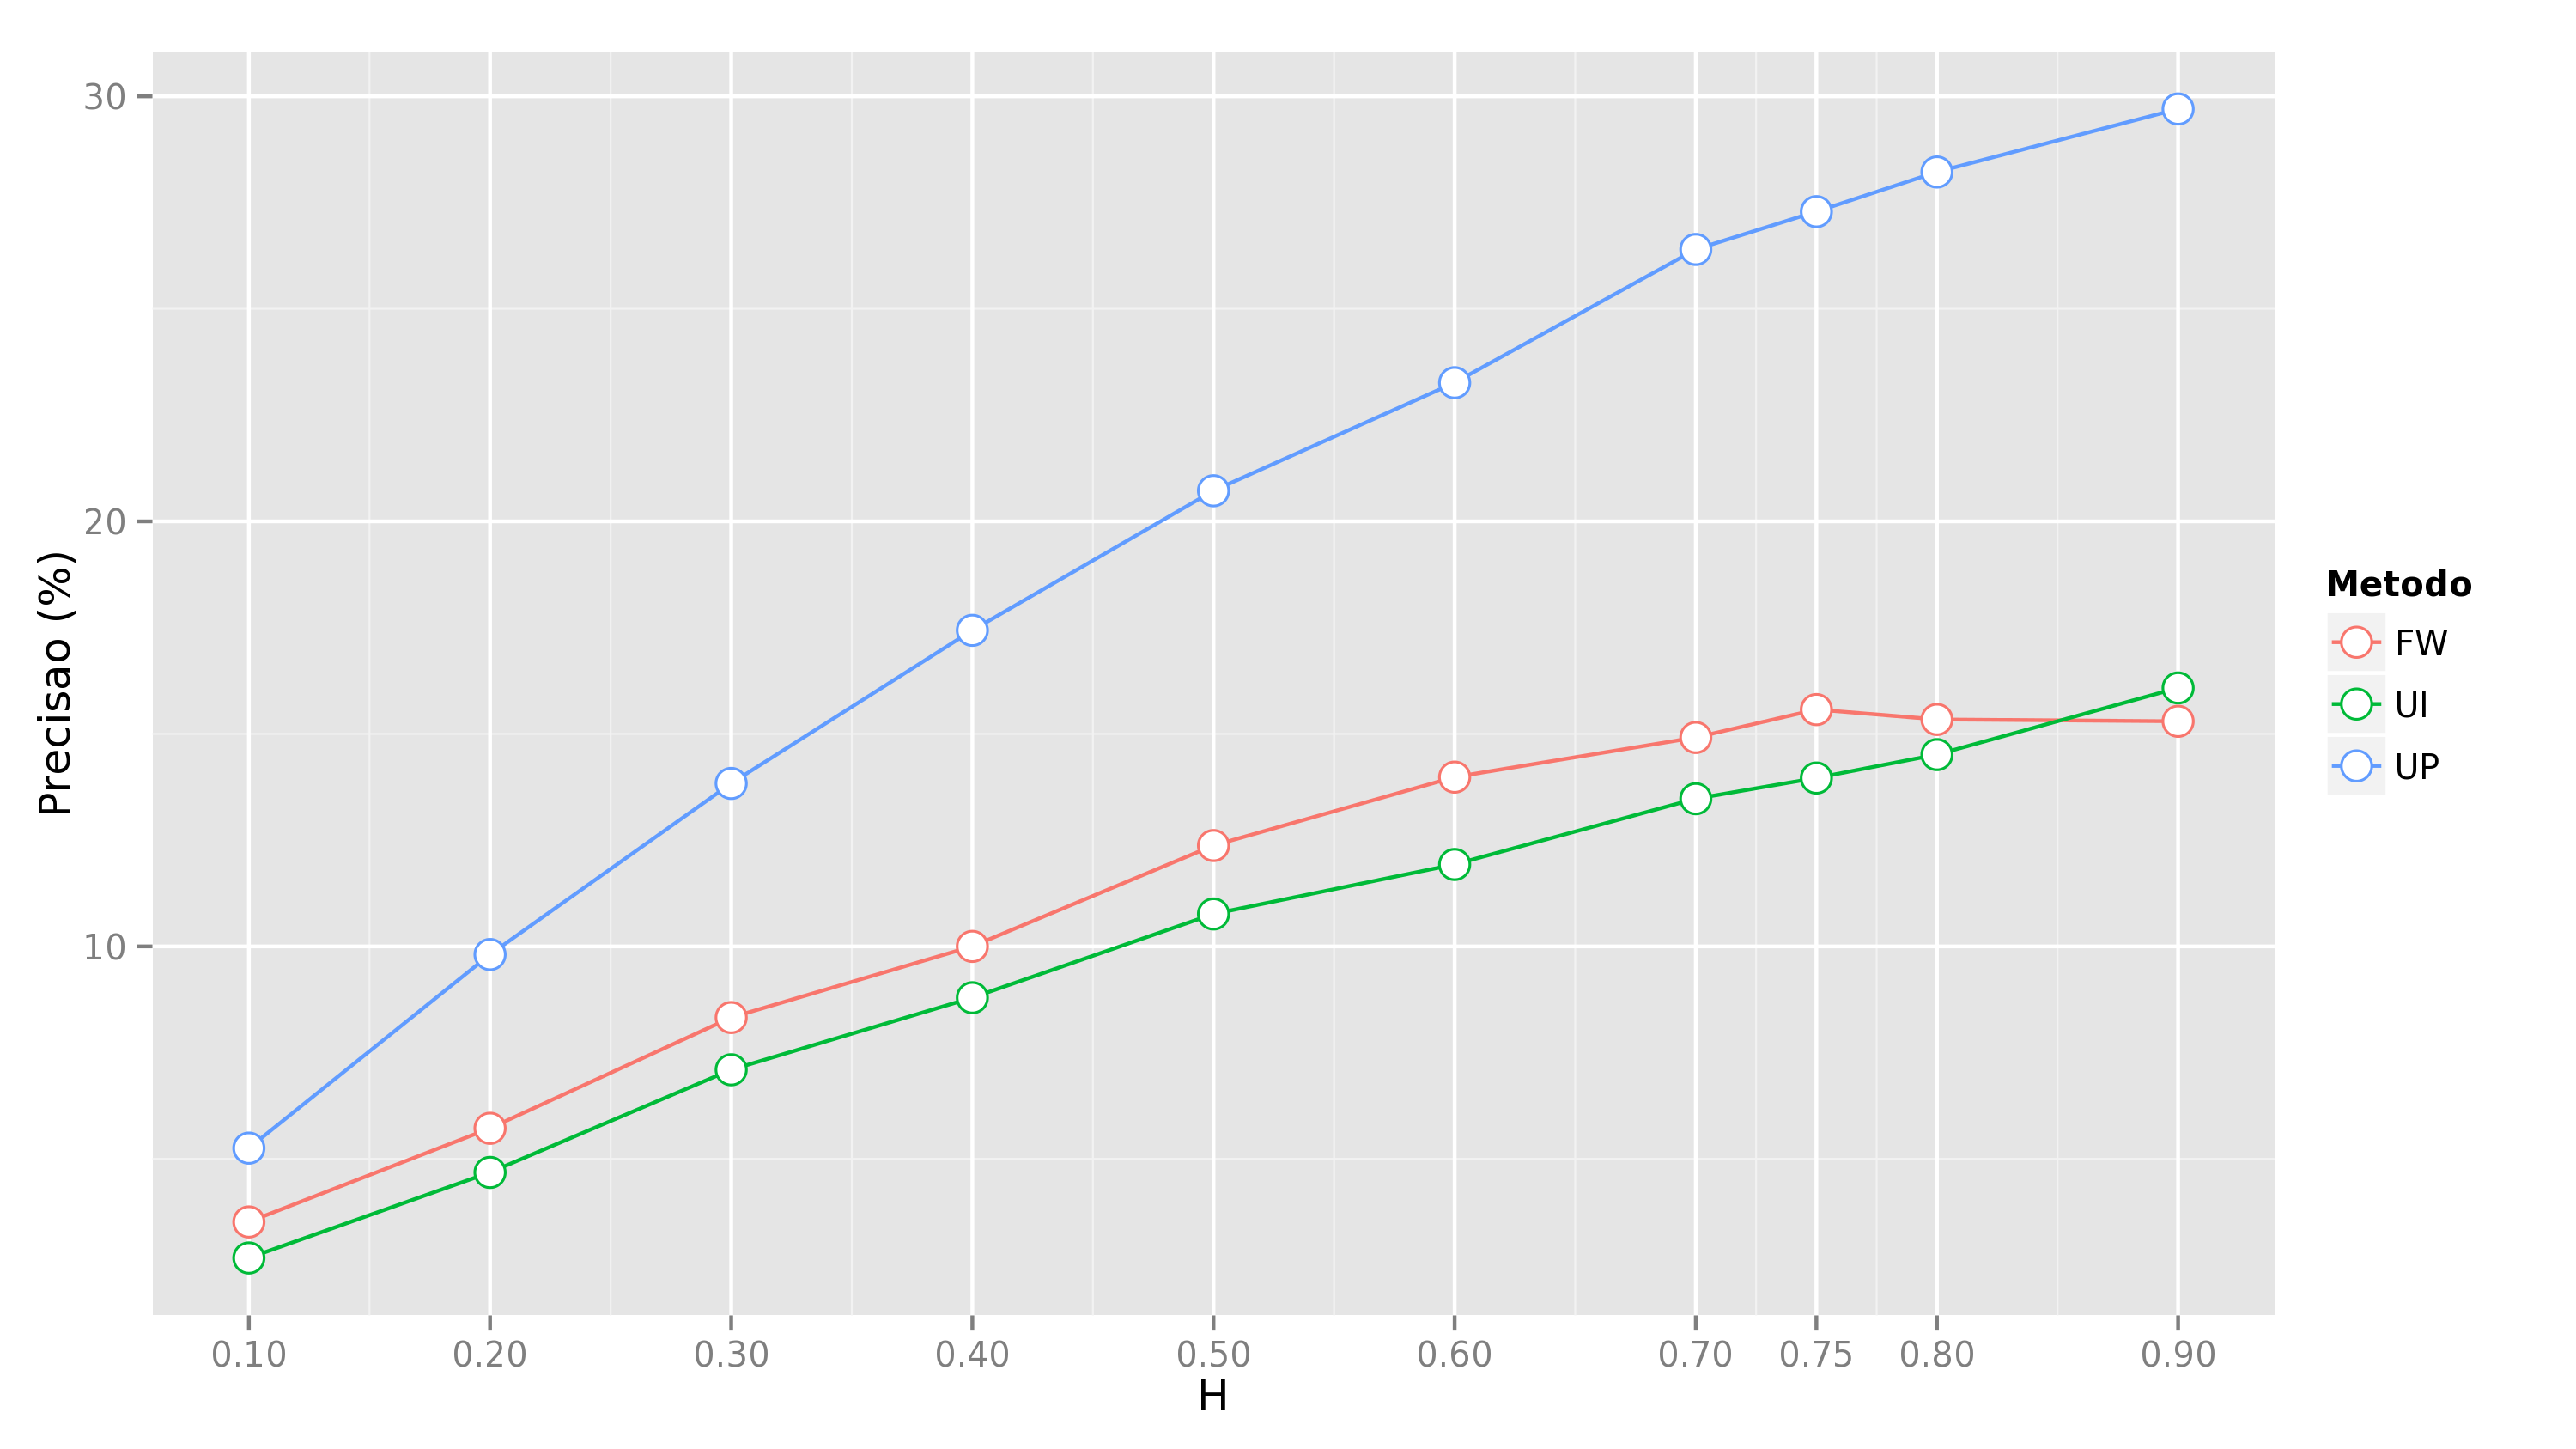
\includegraphics[width=1\textwidth]{img/precision_H}
    \end{center}
    \label{fig:precision_H}
    \caption{Precisão em função do percentual de avaliações ``escondidas'' $H$}
\end{figure}


\begin{figure}[htp]
    \begin{center}
    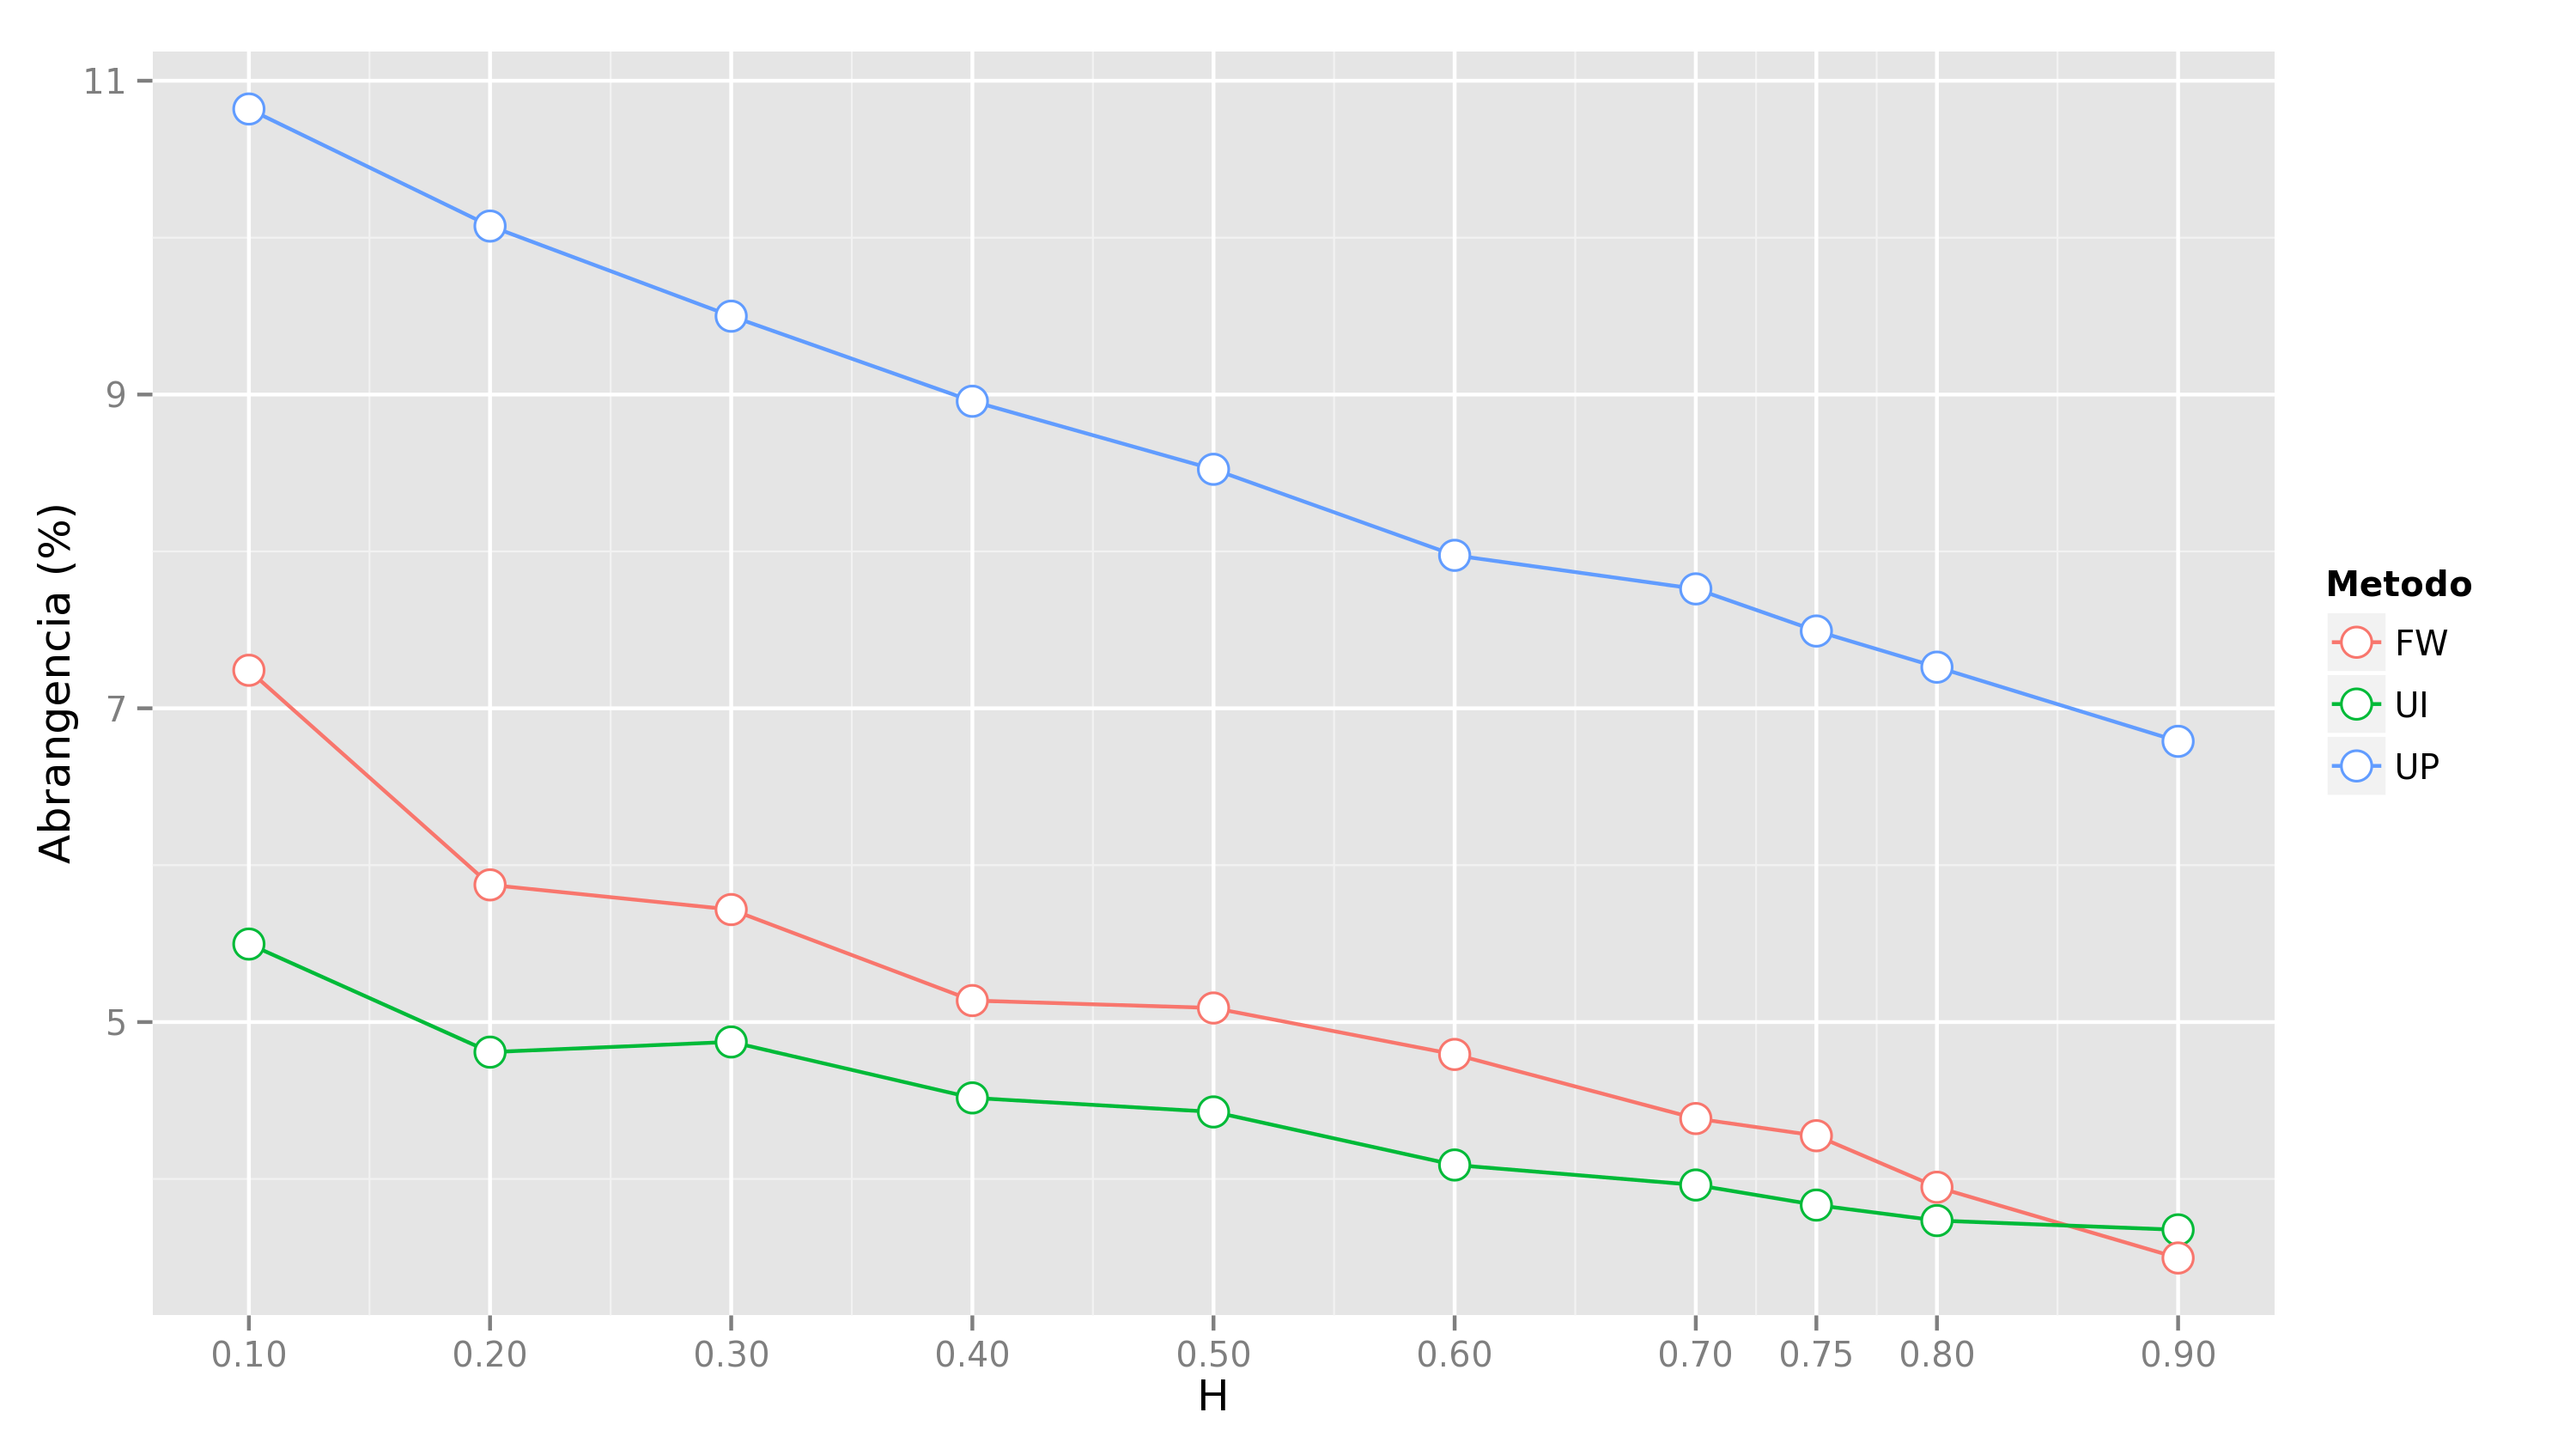
\includegraphics[width=1\textwidth]{img/recall_H}
    \end{center}
    \label{fig:recall_H}
    \caption{Abrangência em função do percentual de avaliações ``escondidas'' $H$}
\end{figure}

\begin{figure}[htp]
    \begin{center}
    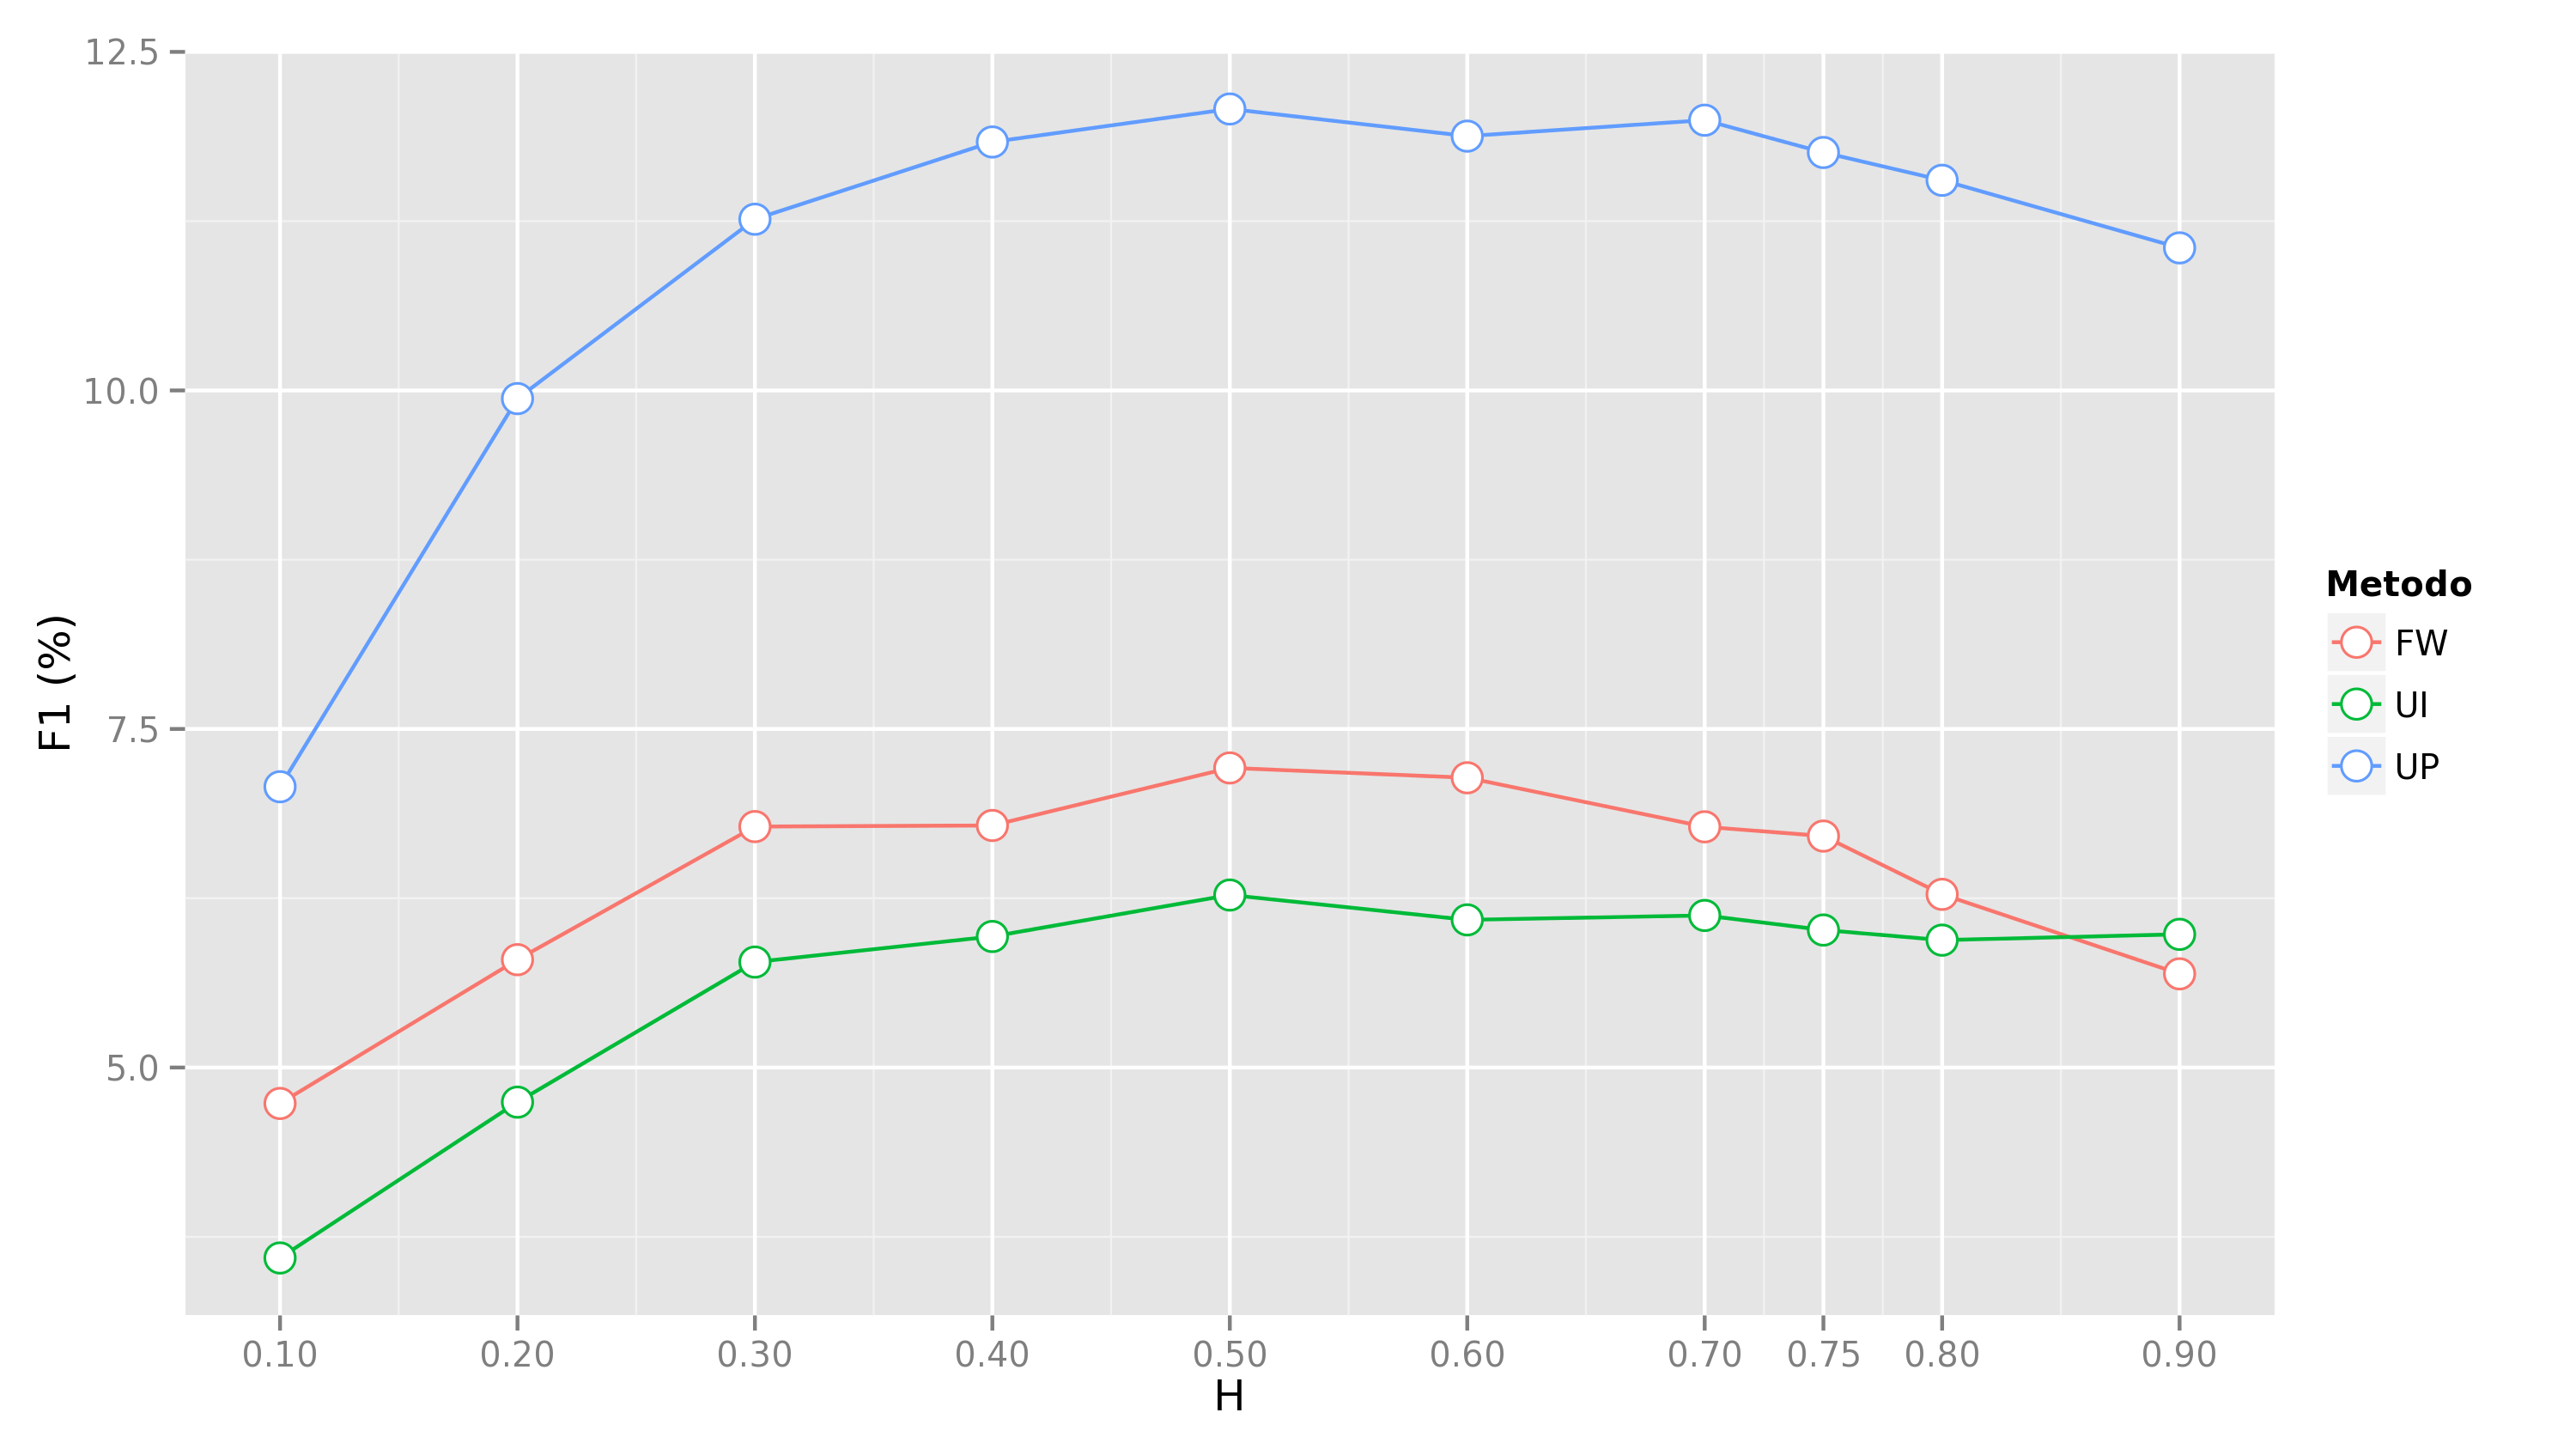
\includegraphics[width=1\textwidth]{img/F1_H}
    \end{center}
    \label{fig:F1_H}
    \caption{Medida $F_1$ em função do percentual de avaliações ``escondidas'' $H$}
\end{figure}

\begin{figure}[htp]
    \begin{center}
    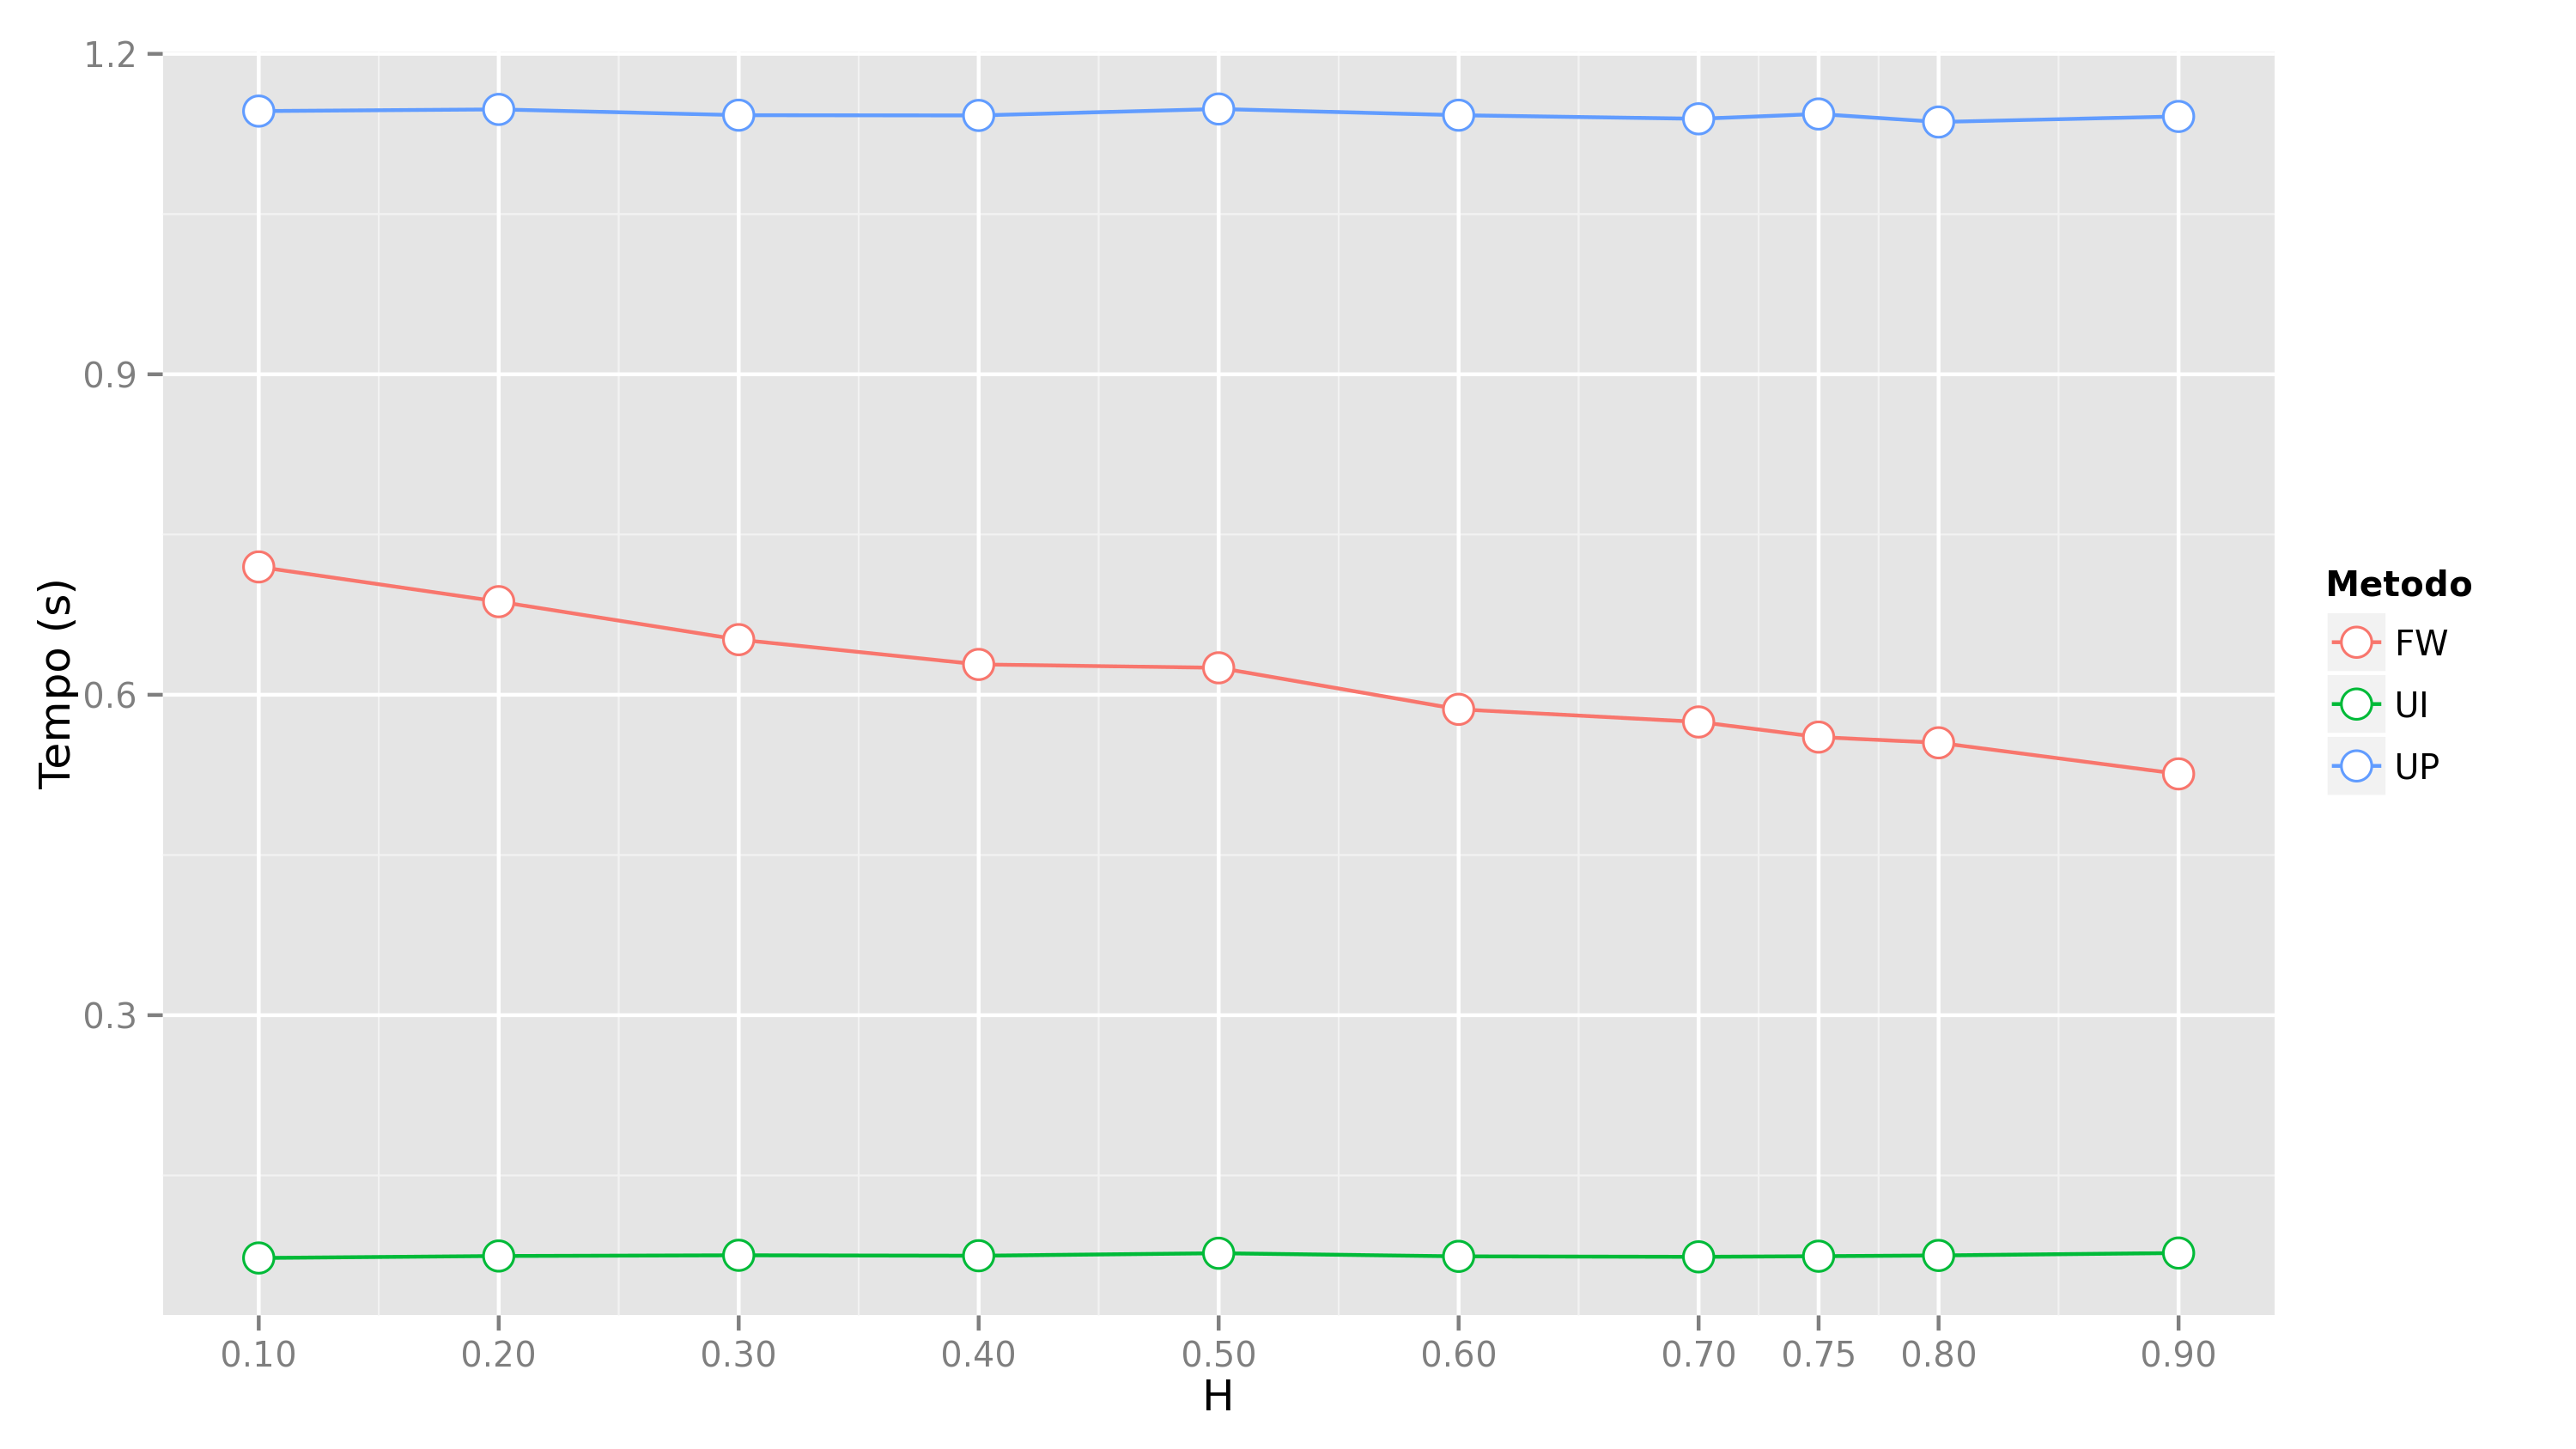
\includegraphics[width=1\textwidth]{img/time_H}
    \end{center}
    \label{fig:time_H}
    \caption{Tempo de execução em função do percentual de avaliações ``escondidas'' $H$}
\end{figure}


\section{Valor mínimo para avaliações positivas $M$} % (fold)
\label{sec:valor_m_nimo_para_avalia_es_positivas_}


\begin{figure}[htp]
    \begin{center}
    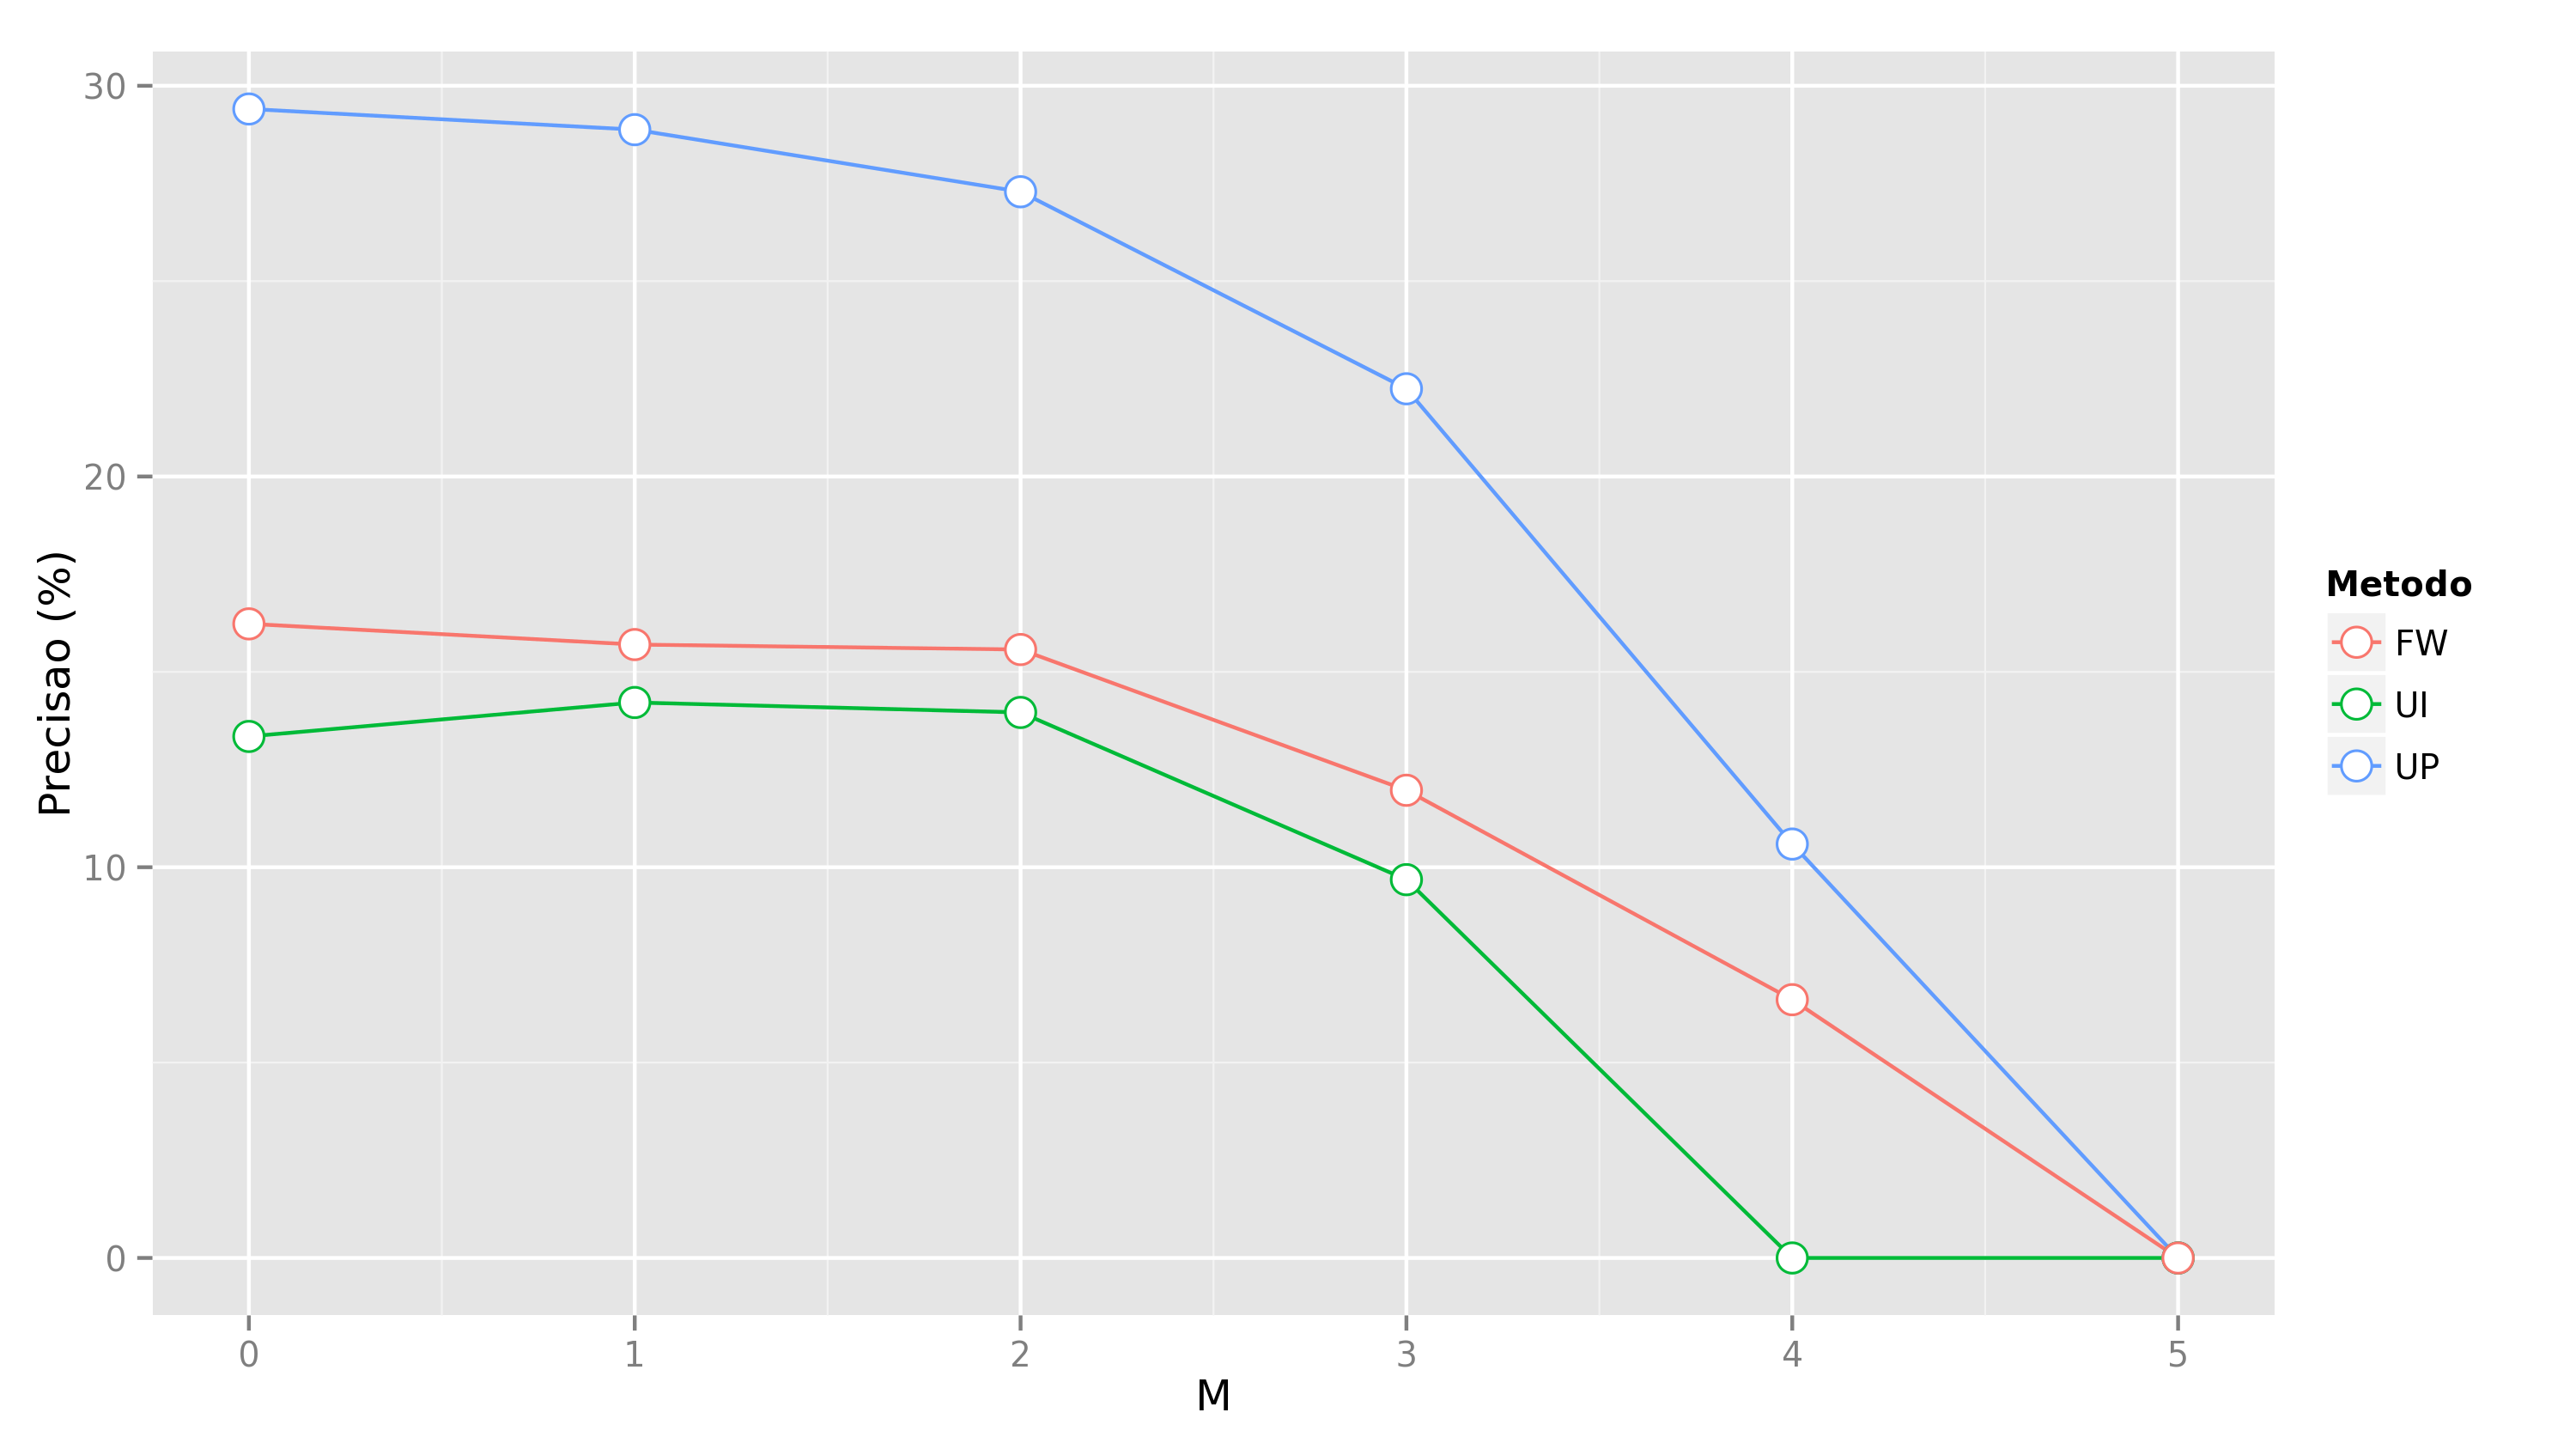
\includegraphics[width=1\textwidth]{img/precision_M}
    \end{center}
    \label{fig:precision_M}
    \caption{Precisão em função do valor mínimo para avaliações positivas $M$}
\end{figure}


\begin{figure}[htp]
    \begin{center}
    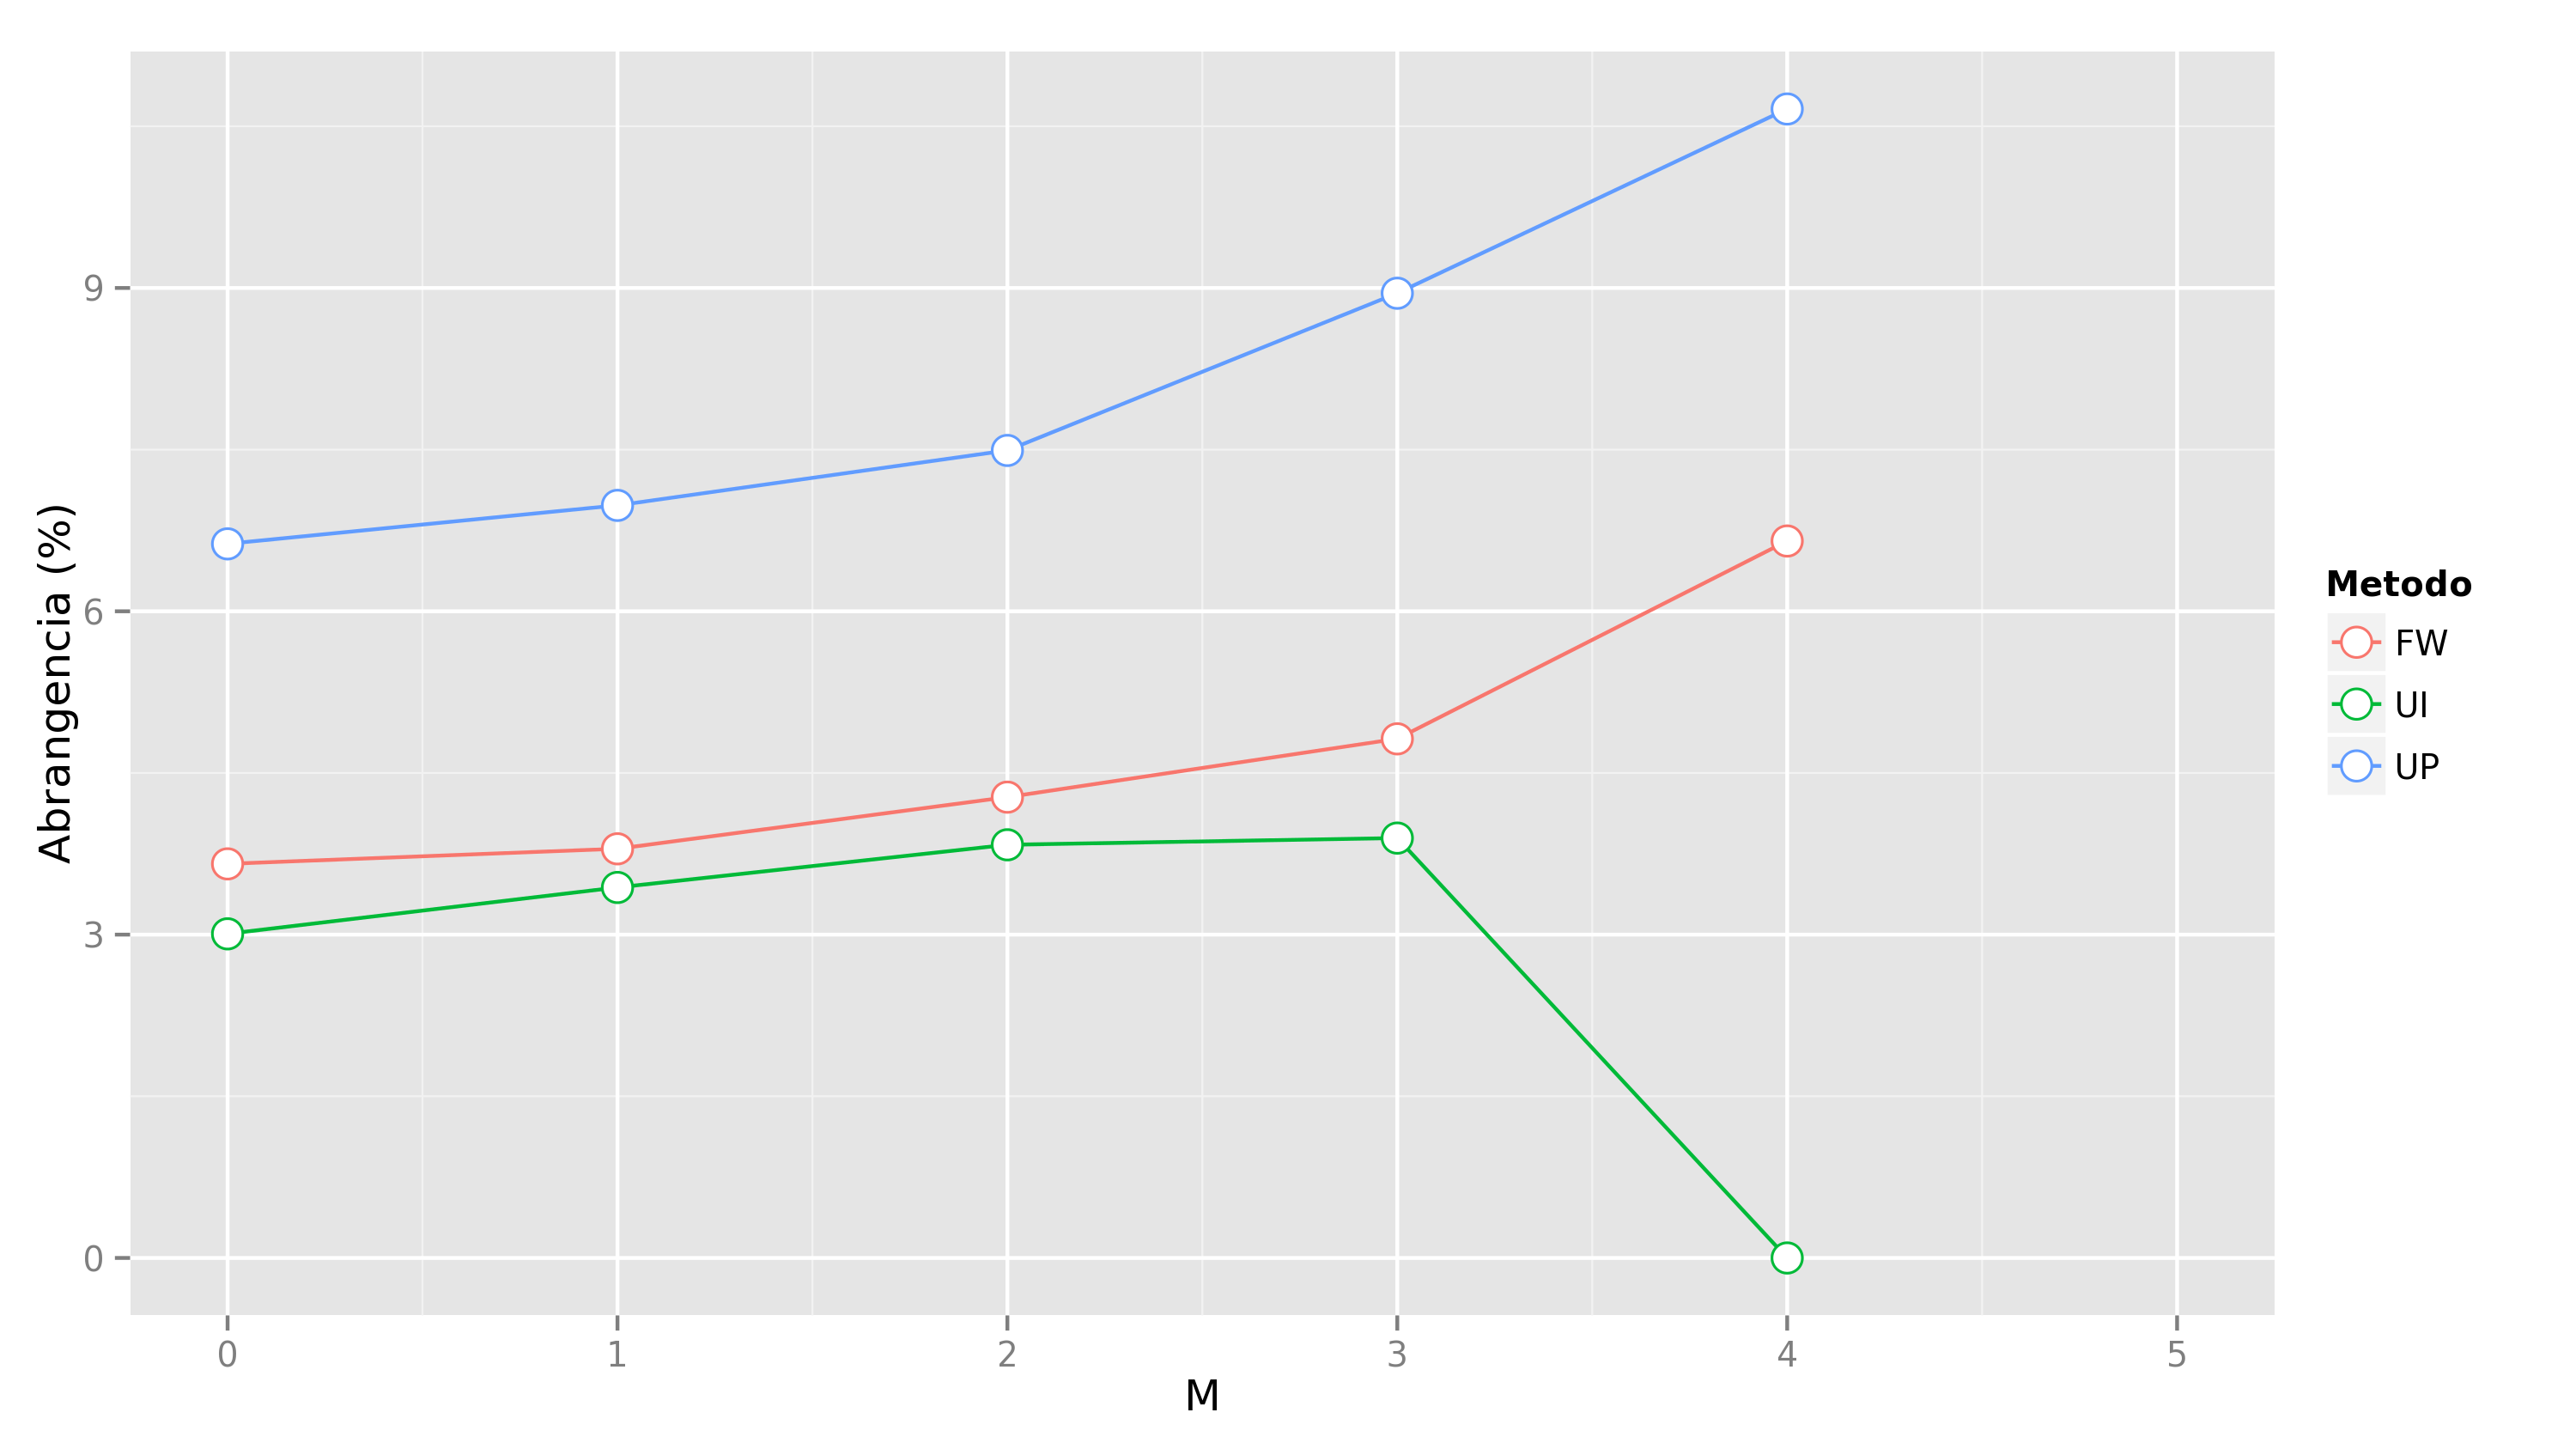
\includegraphics[width=1\textwidth]{img/recall_M}
    \end{center}
    \label{fig:recall_M}
    \caption{Abrangência em função do valor mínimo para avaliações positivas $M$}
\end{figure}

\begin{figure}[htp]
    \begin{center}
    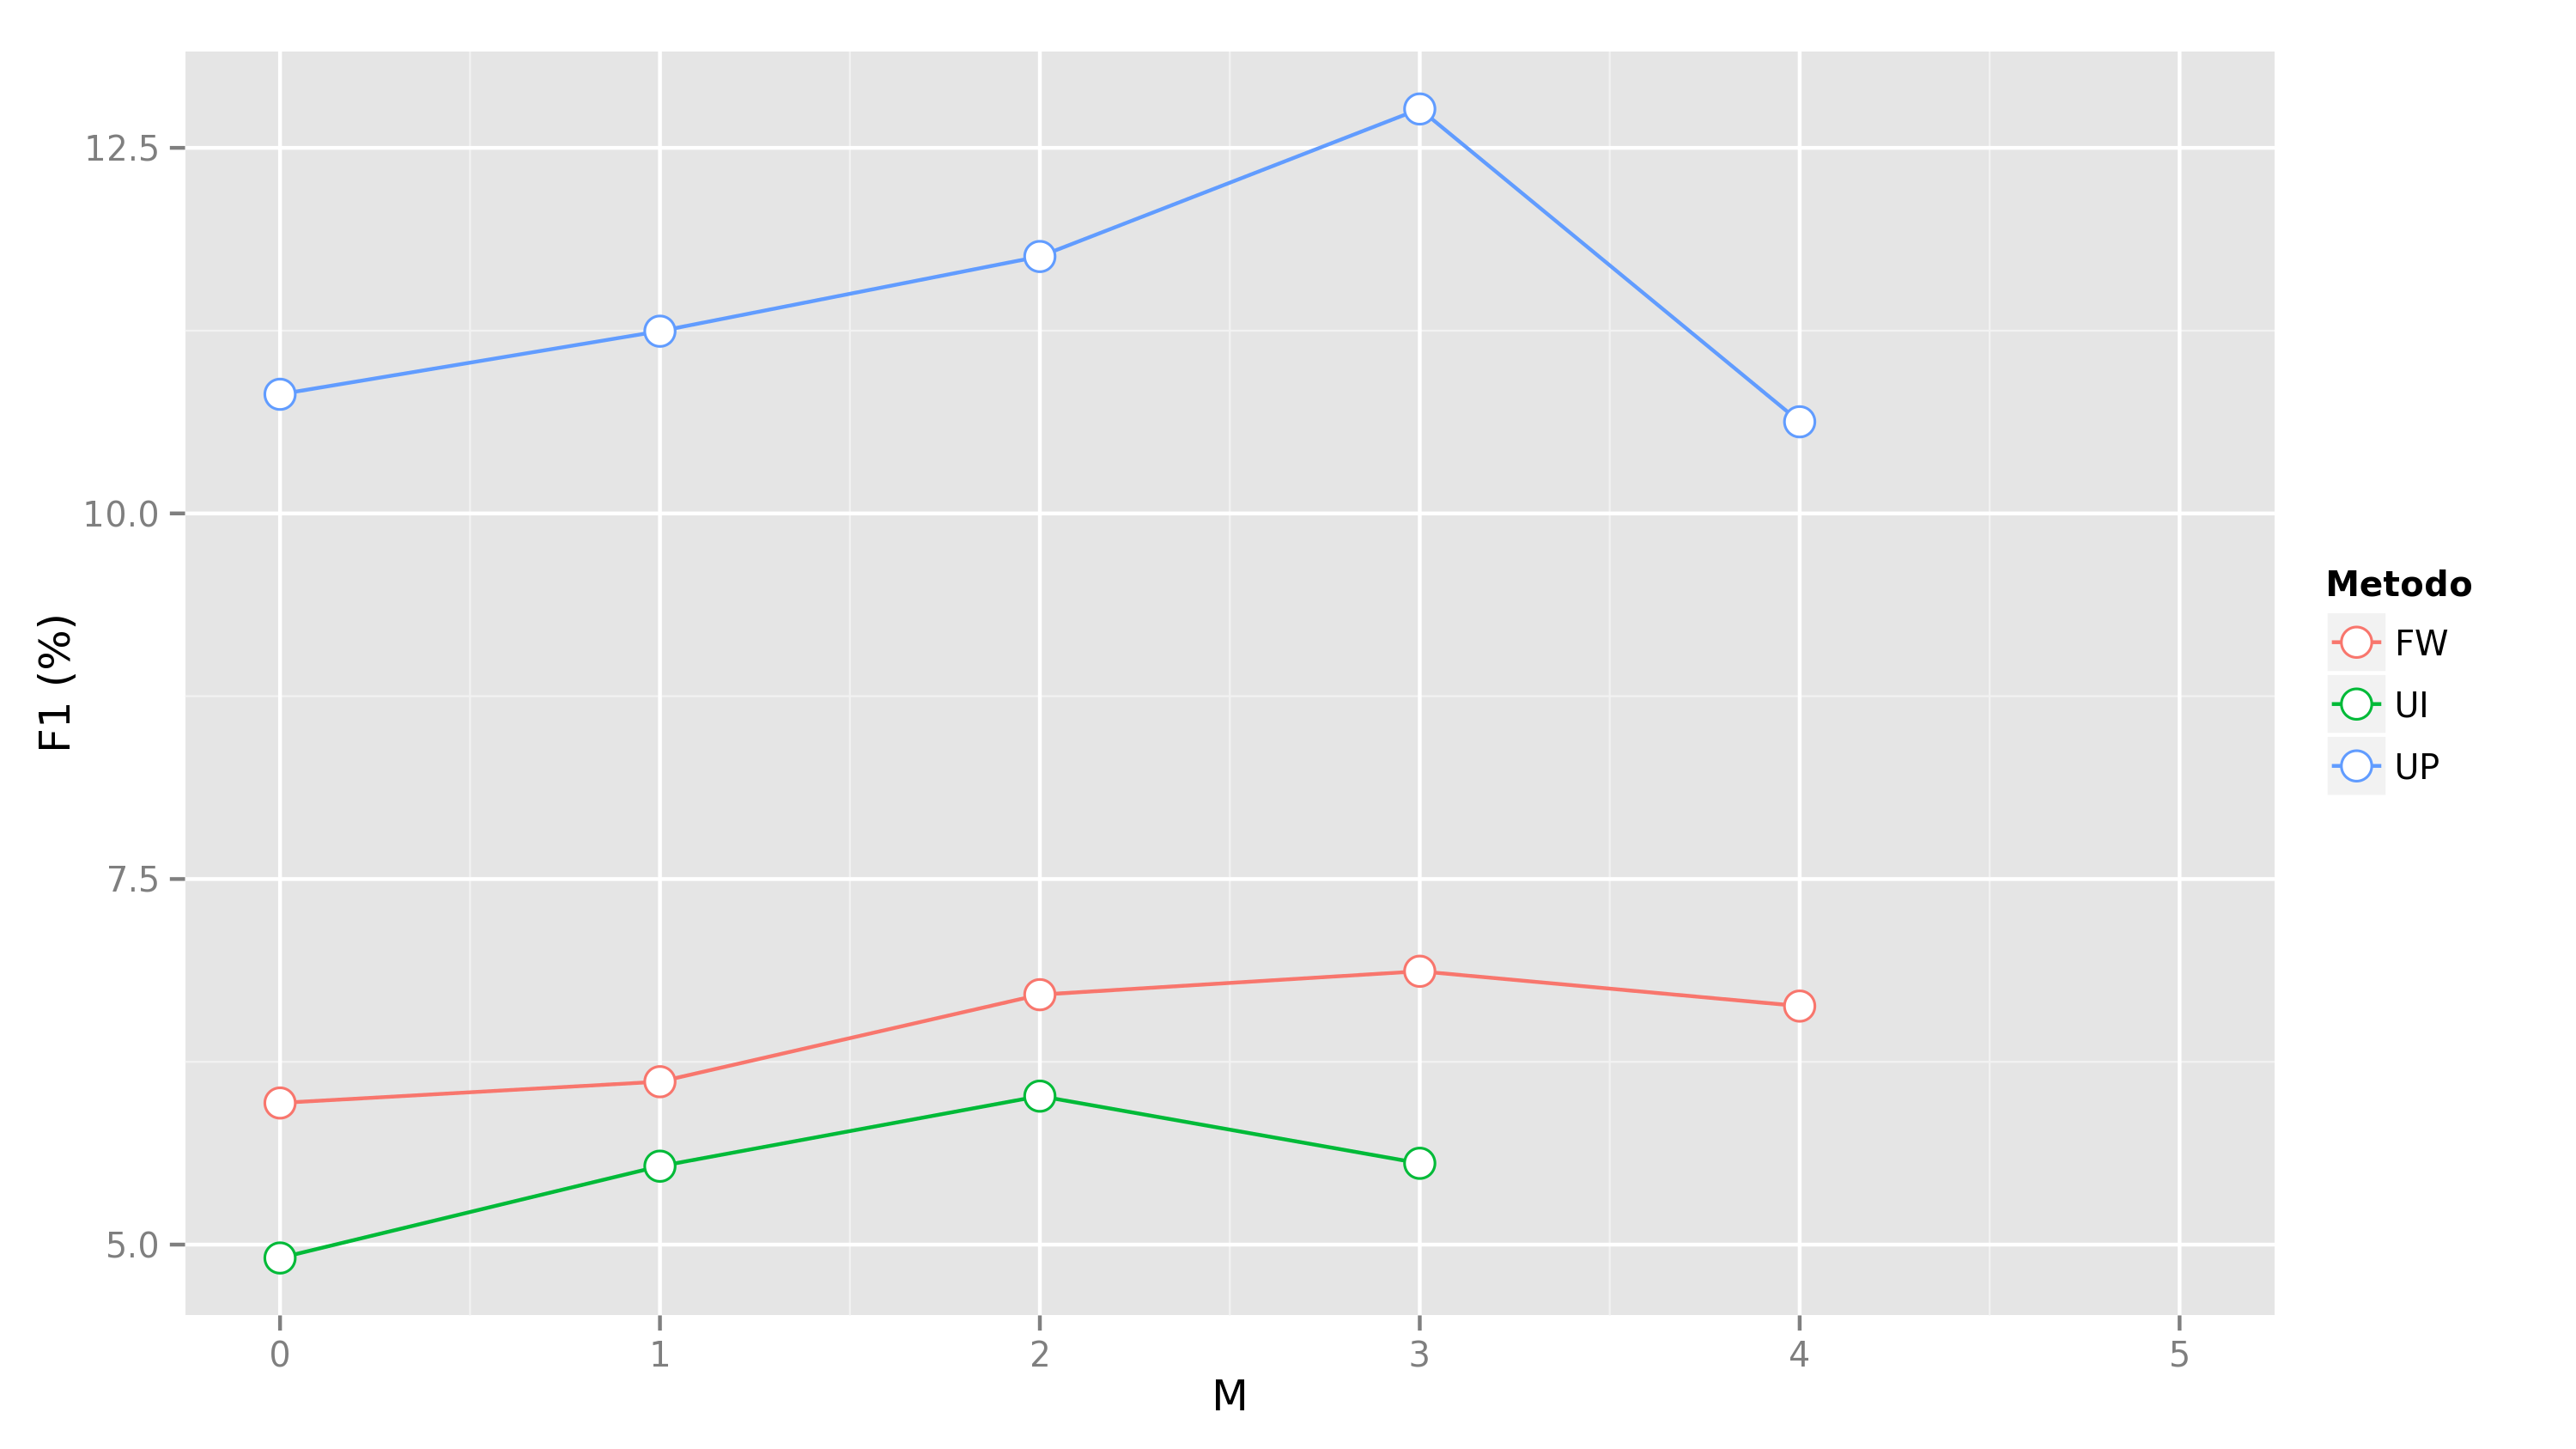
\includegraphics[width=1\textwidth]{img/F1_M}
    \end{center}
    \label{fig:F1_M}
    \caption{Medida $F_1$ em função do valor mínimo para avaliações positivas $M$}
\end{figure}

\begin{figure}[htp]
    \begin{center}
    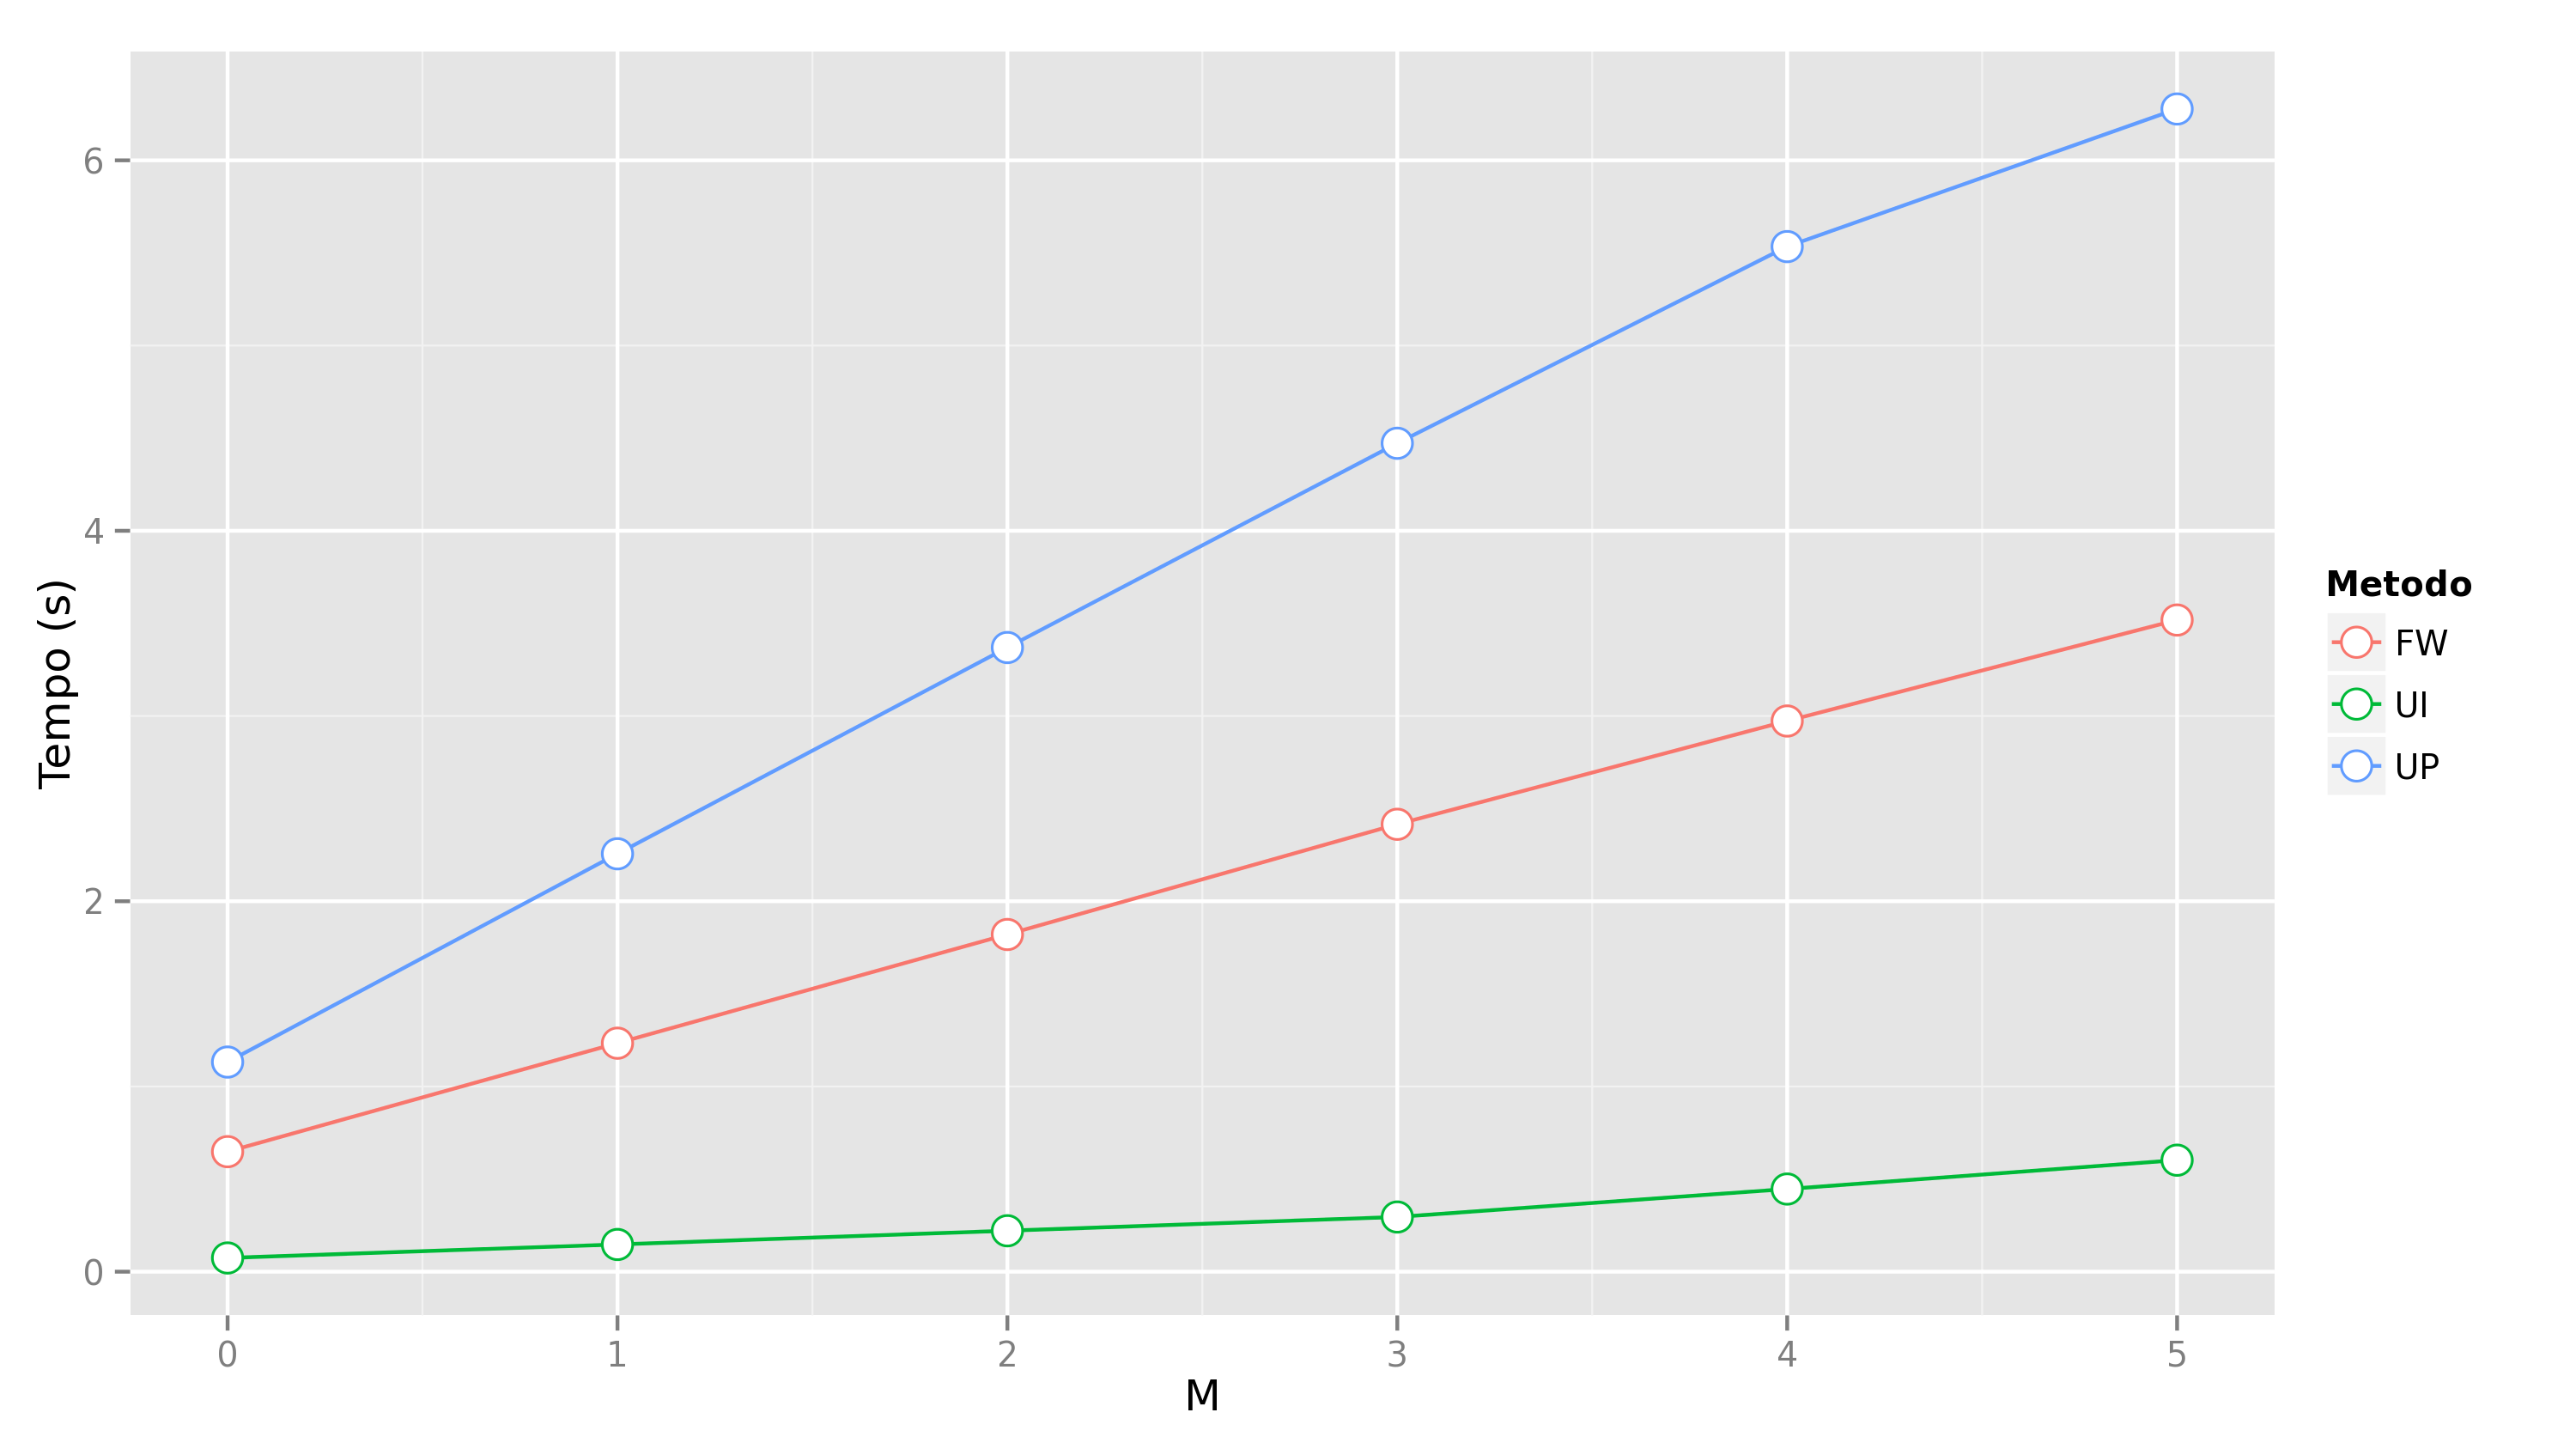
\includegraphics[width=1\textwidth]{img/time_M}
    \end{center}
    \label{fig:time_M}
    \caption{Tempo de execução em função do valor mínimo para avaliações positivas $M$}
\end{figure}

\section{Número de vizinhos mais próximos $k$} % (fold)
\label{sec:n_mero_de_vizinhos_mais_pr_ximos_}


\begin{figure}[htp]
    \begin{center}
    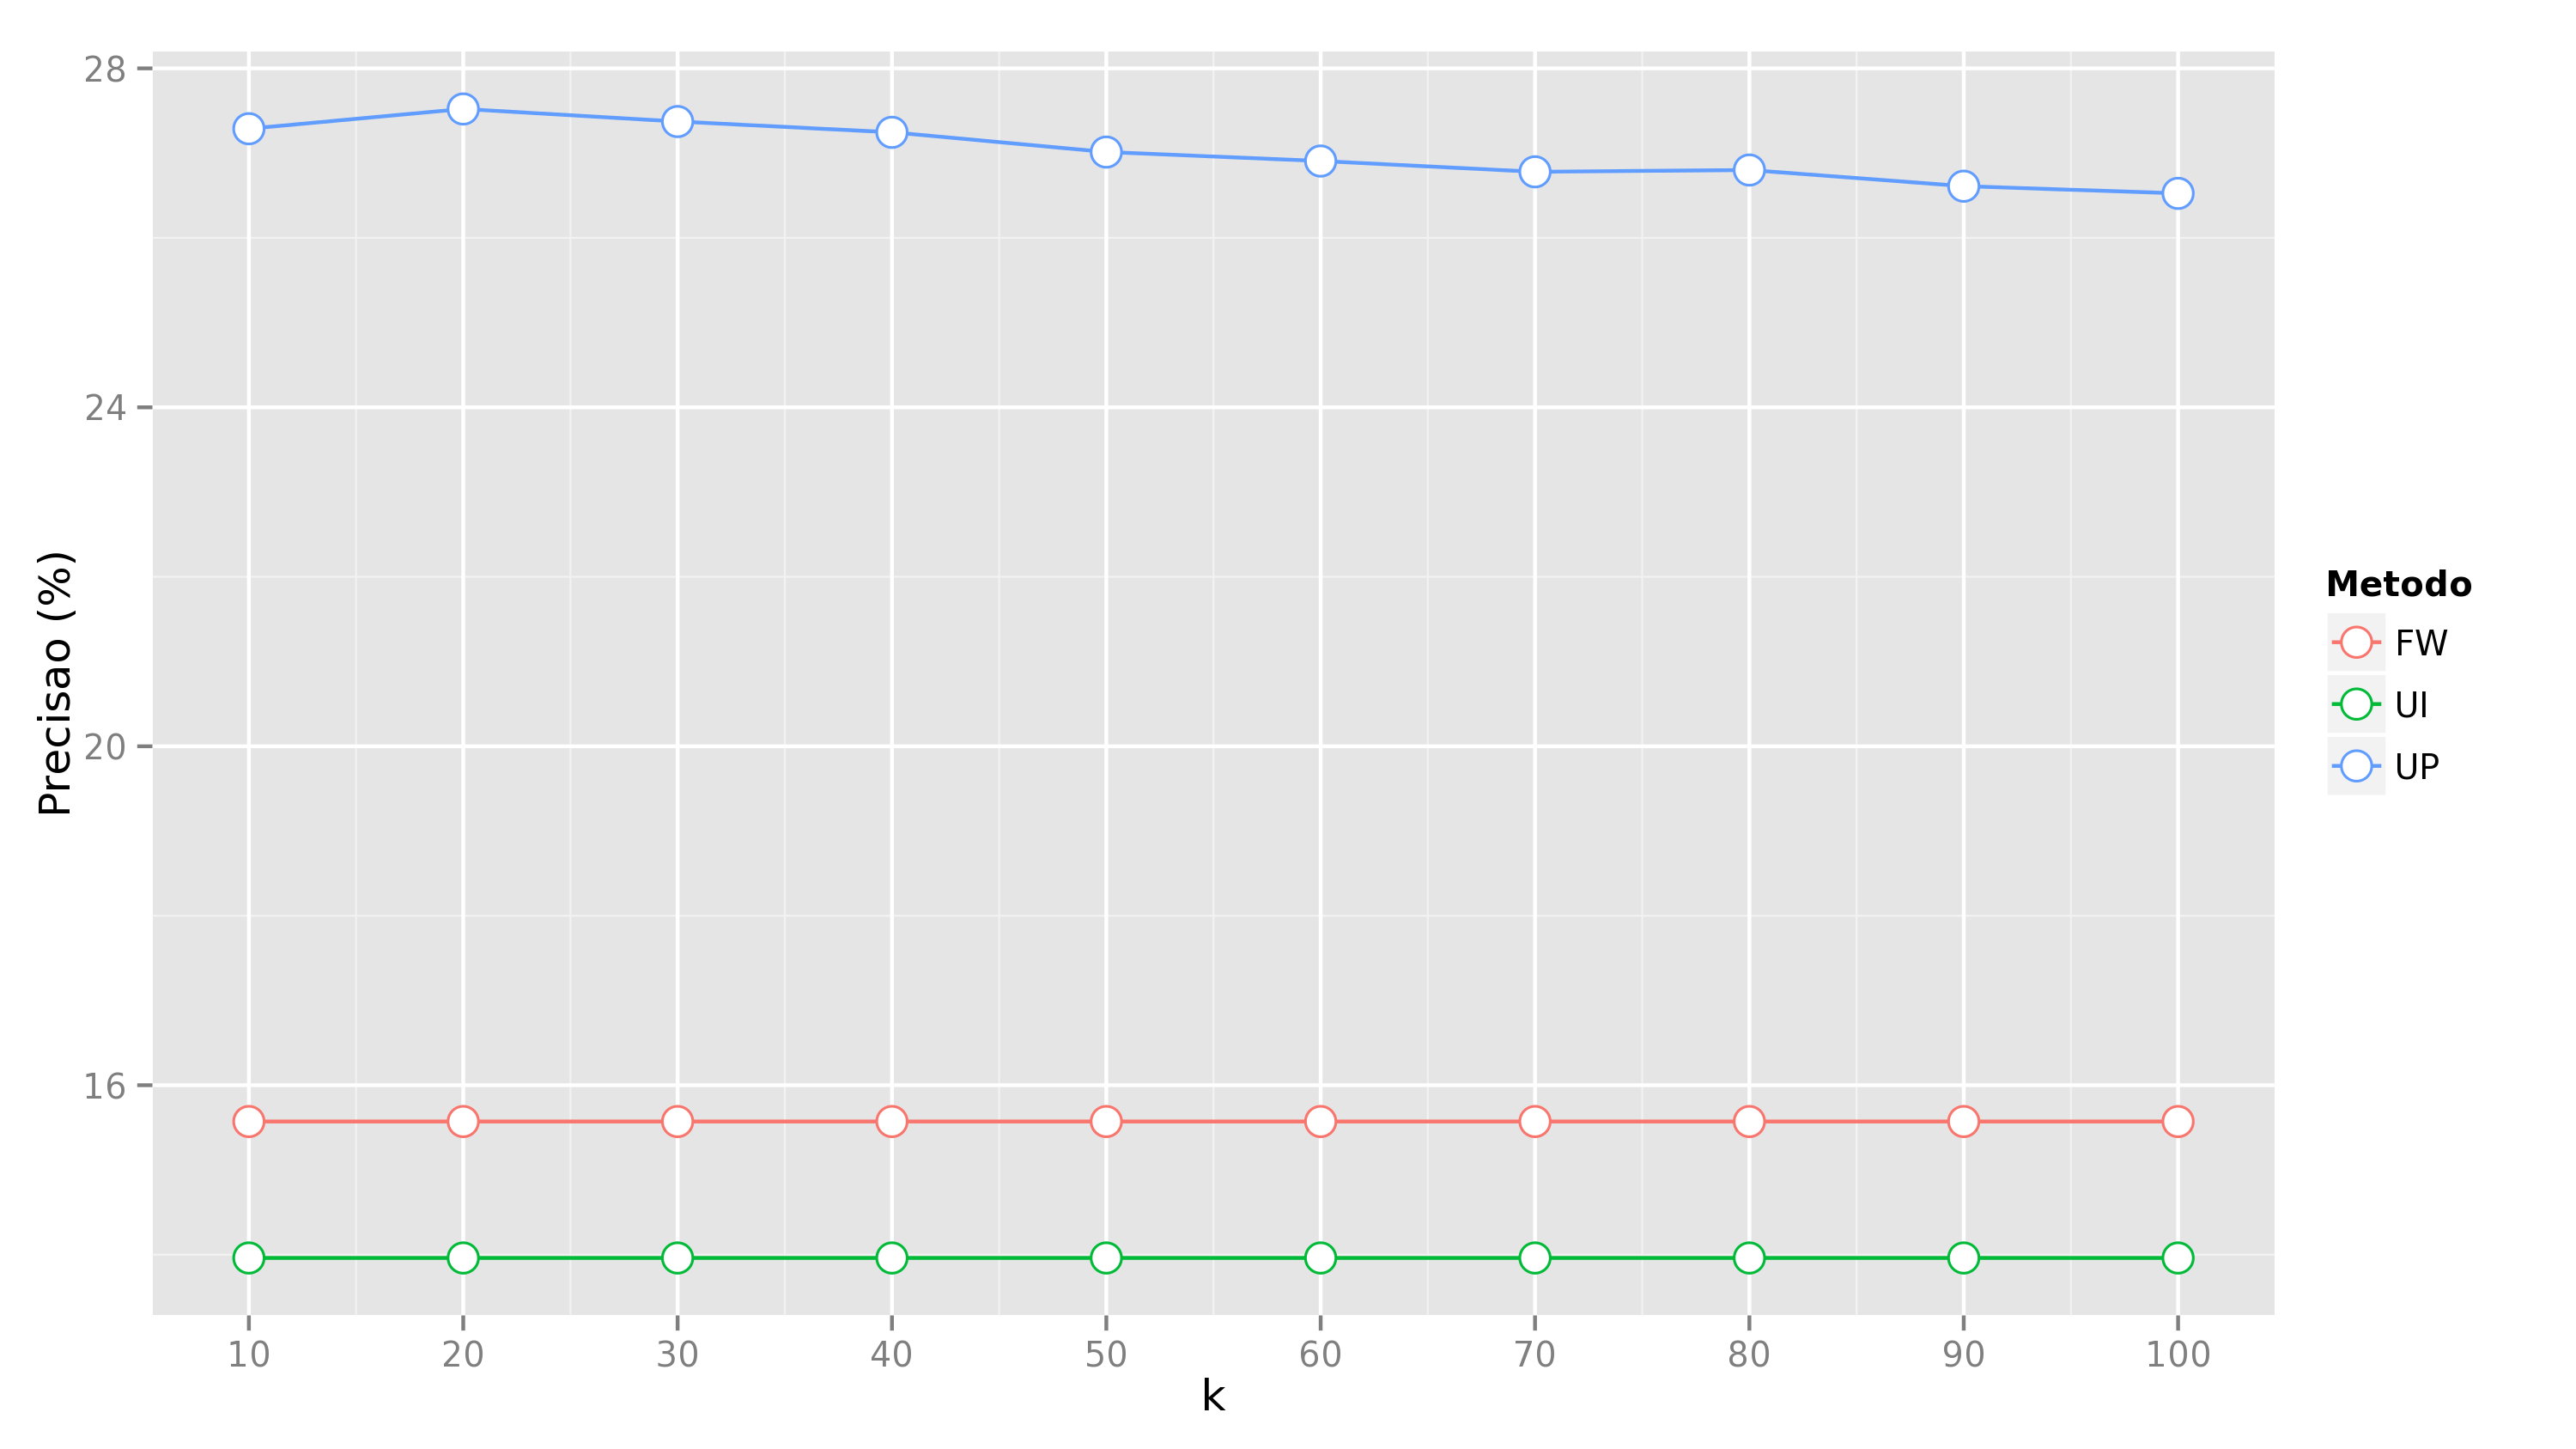
\includegraphics[width=1\textwidth]{img/precision_k}
    \end{center}
    \label{fig:precision_k}
    \caption{Precisão em função do número de vizinhos mais próximos $k$}
\end{figure}


\begin{figure}[htp]
    \begin{center}
    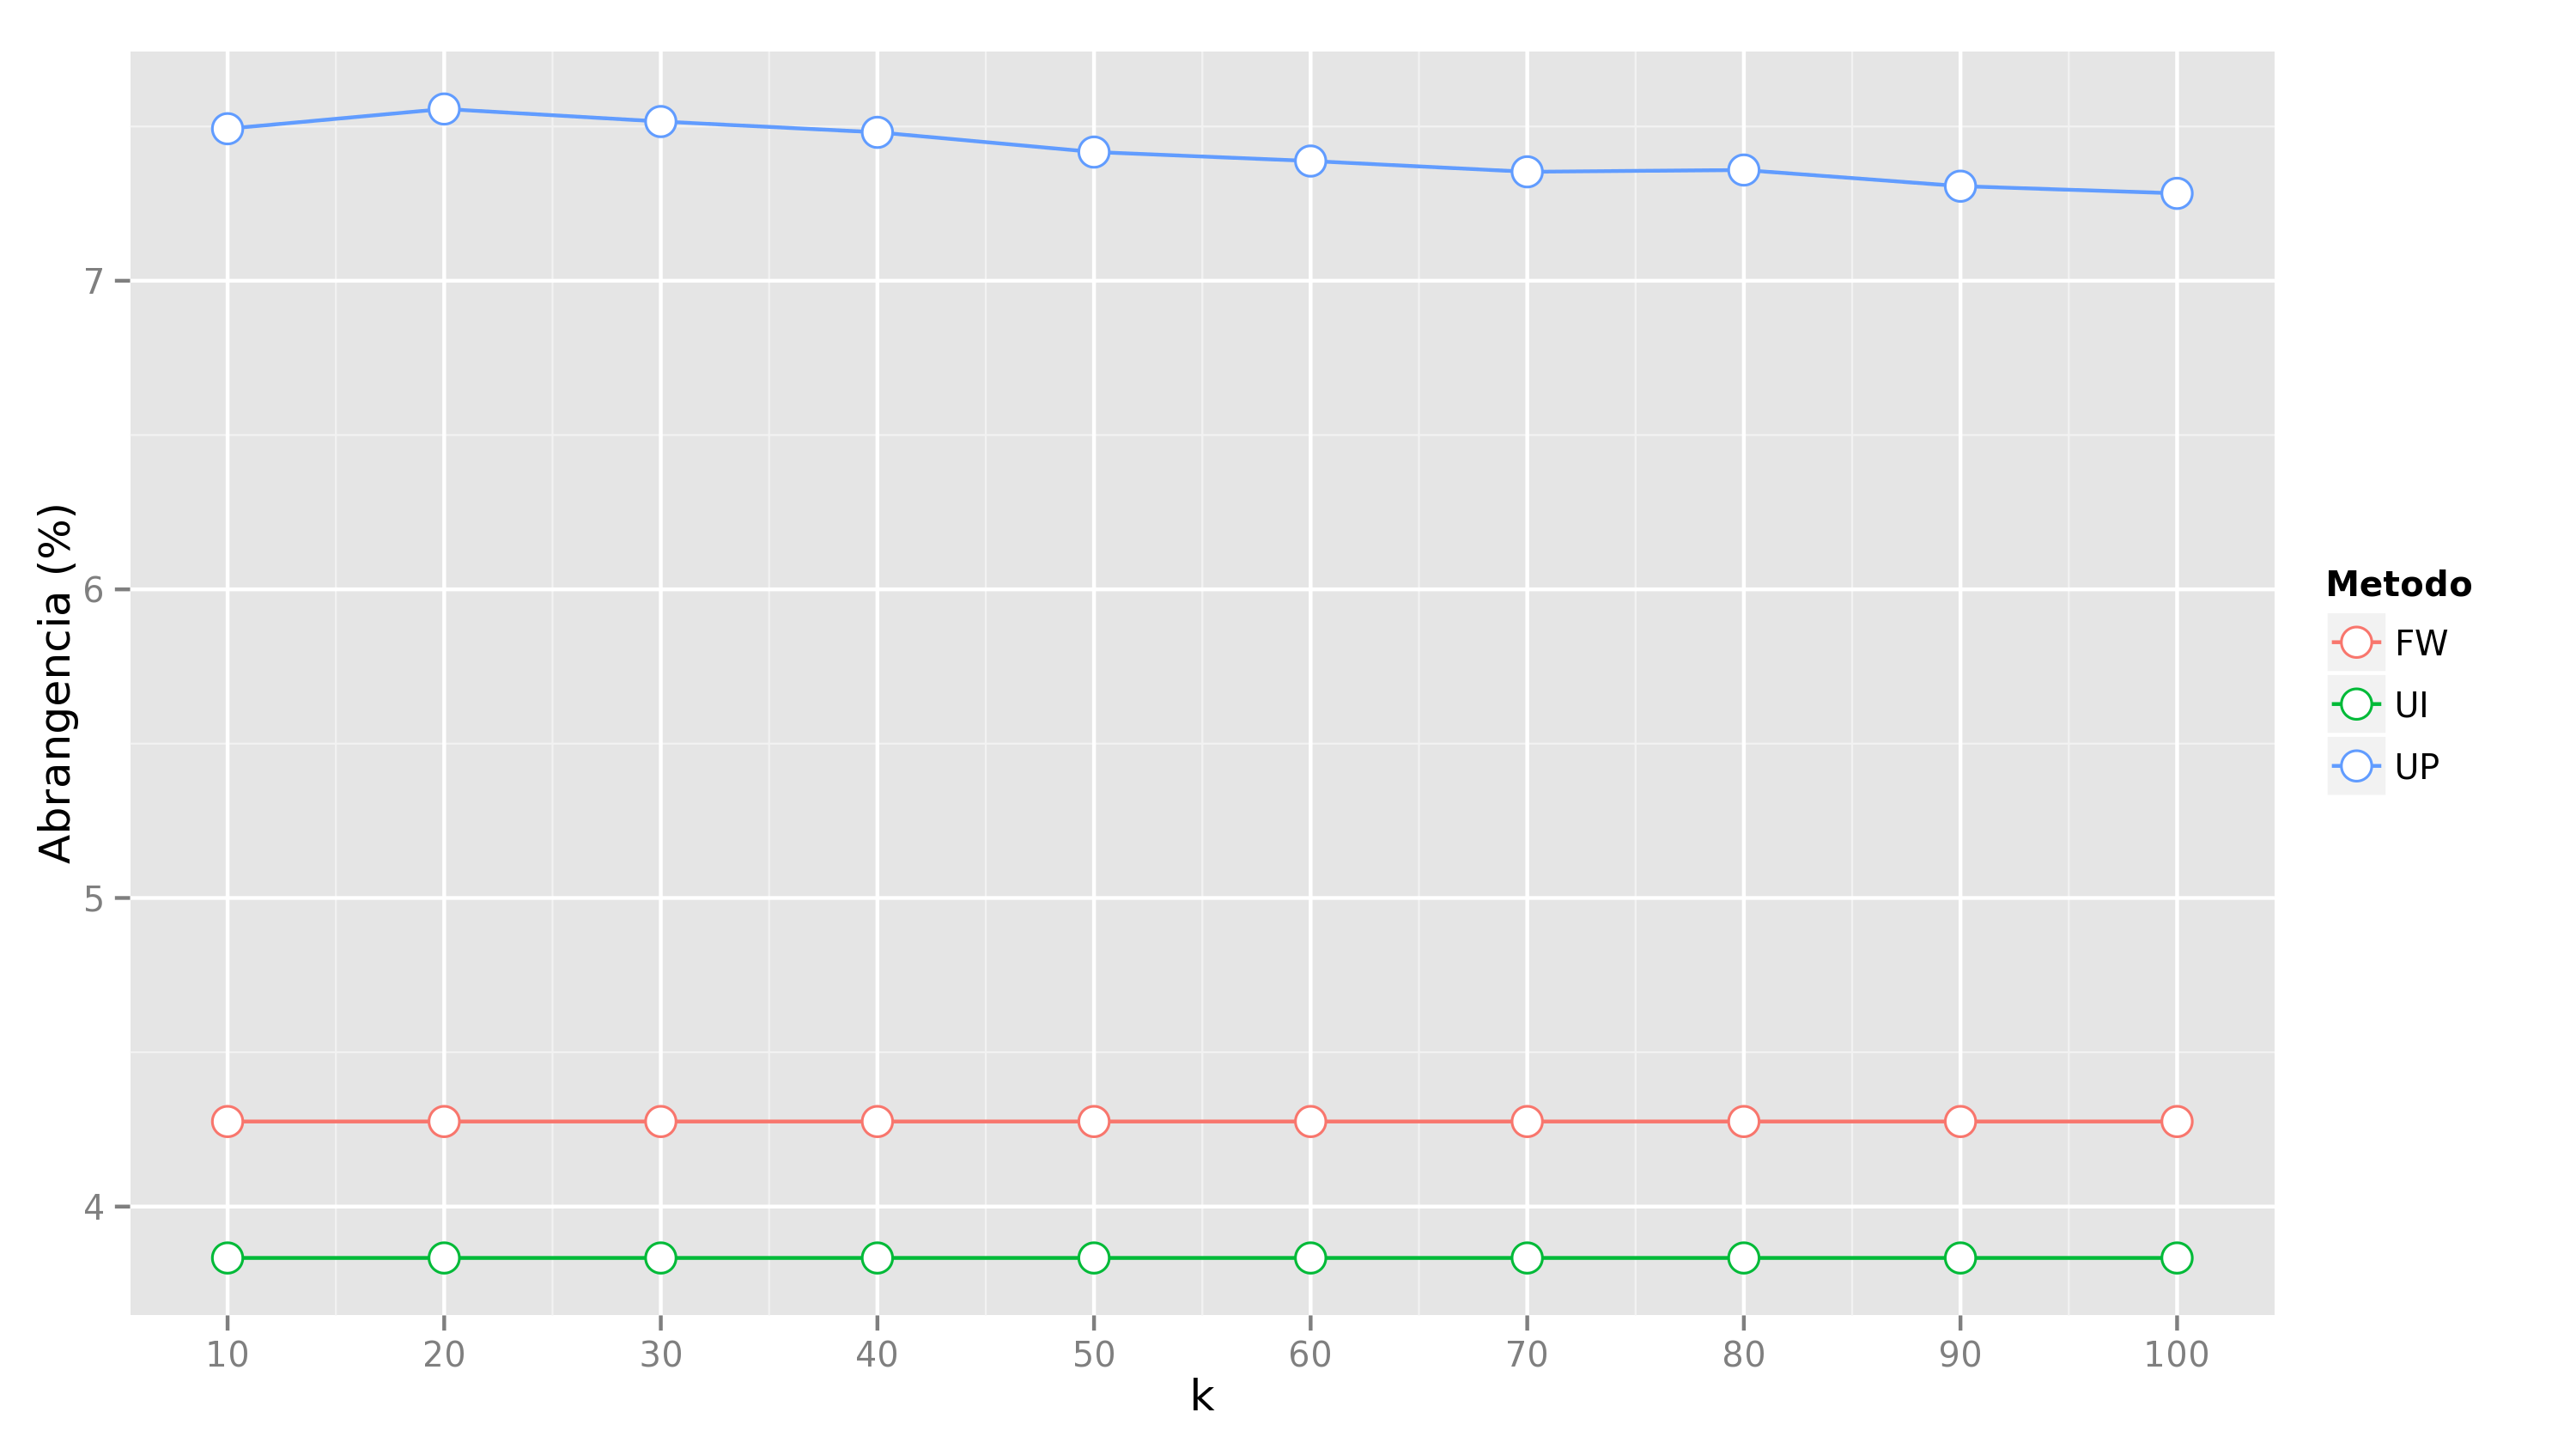
\includegraphics[width=1\textwidth]{img/recall_k}
    \end{center}
    \label{fig:recall_k}
    \caption{Abrangência em função do número de vizinhos mais próximos $k$}
\end{figure}

\begin{figure}[htp]
    \begin{center}
    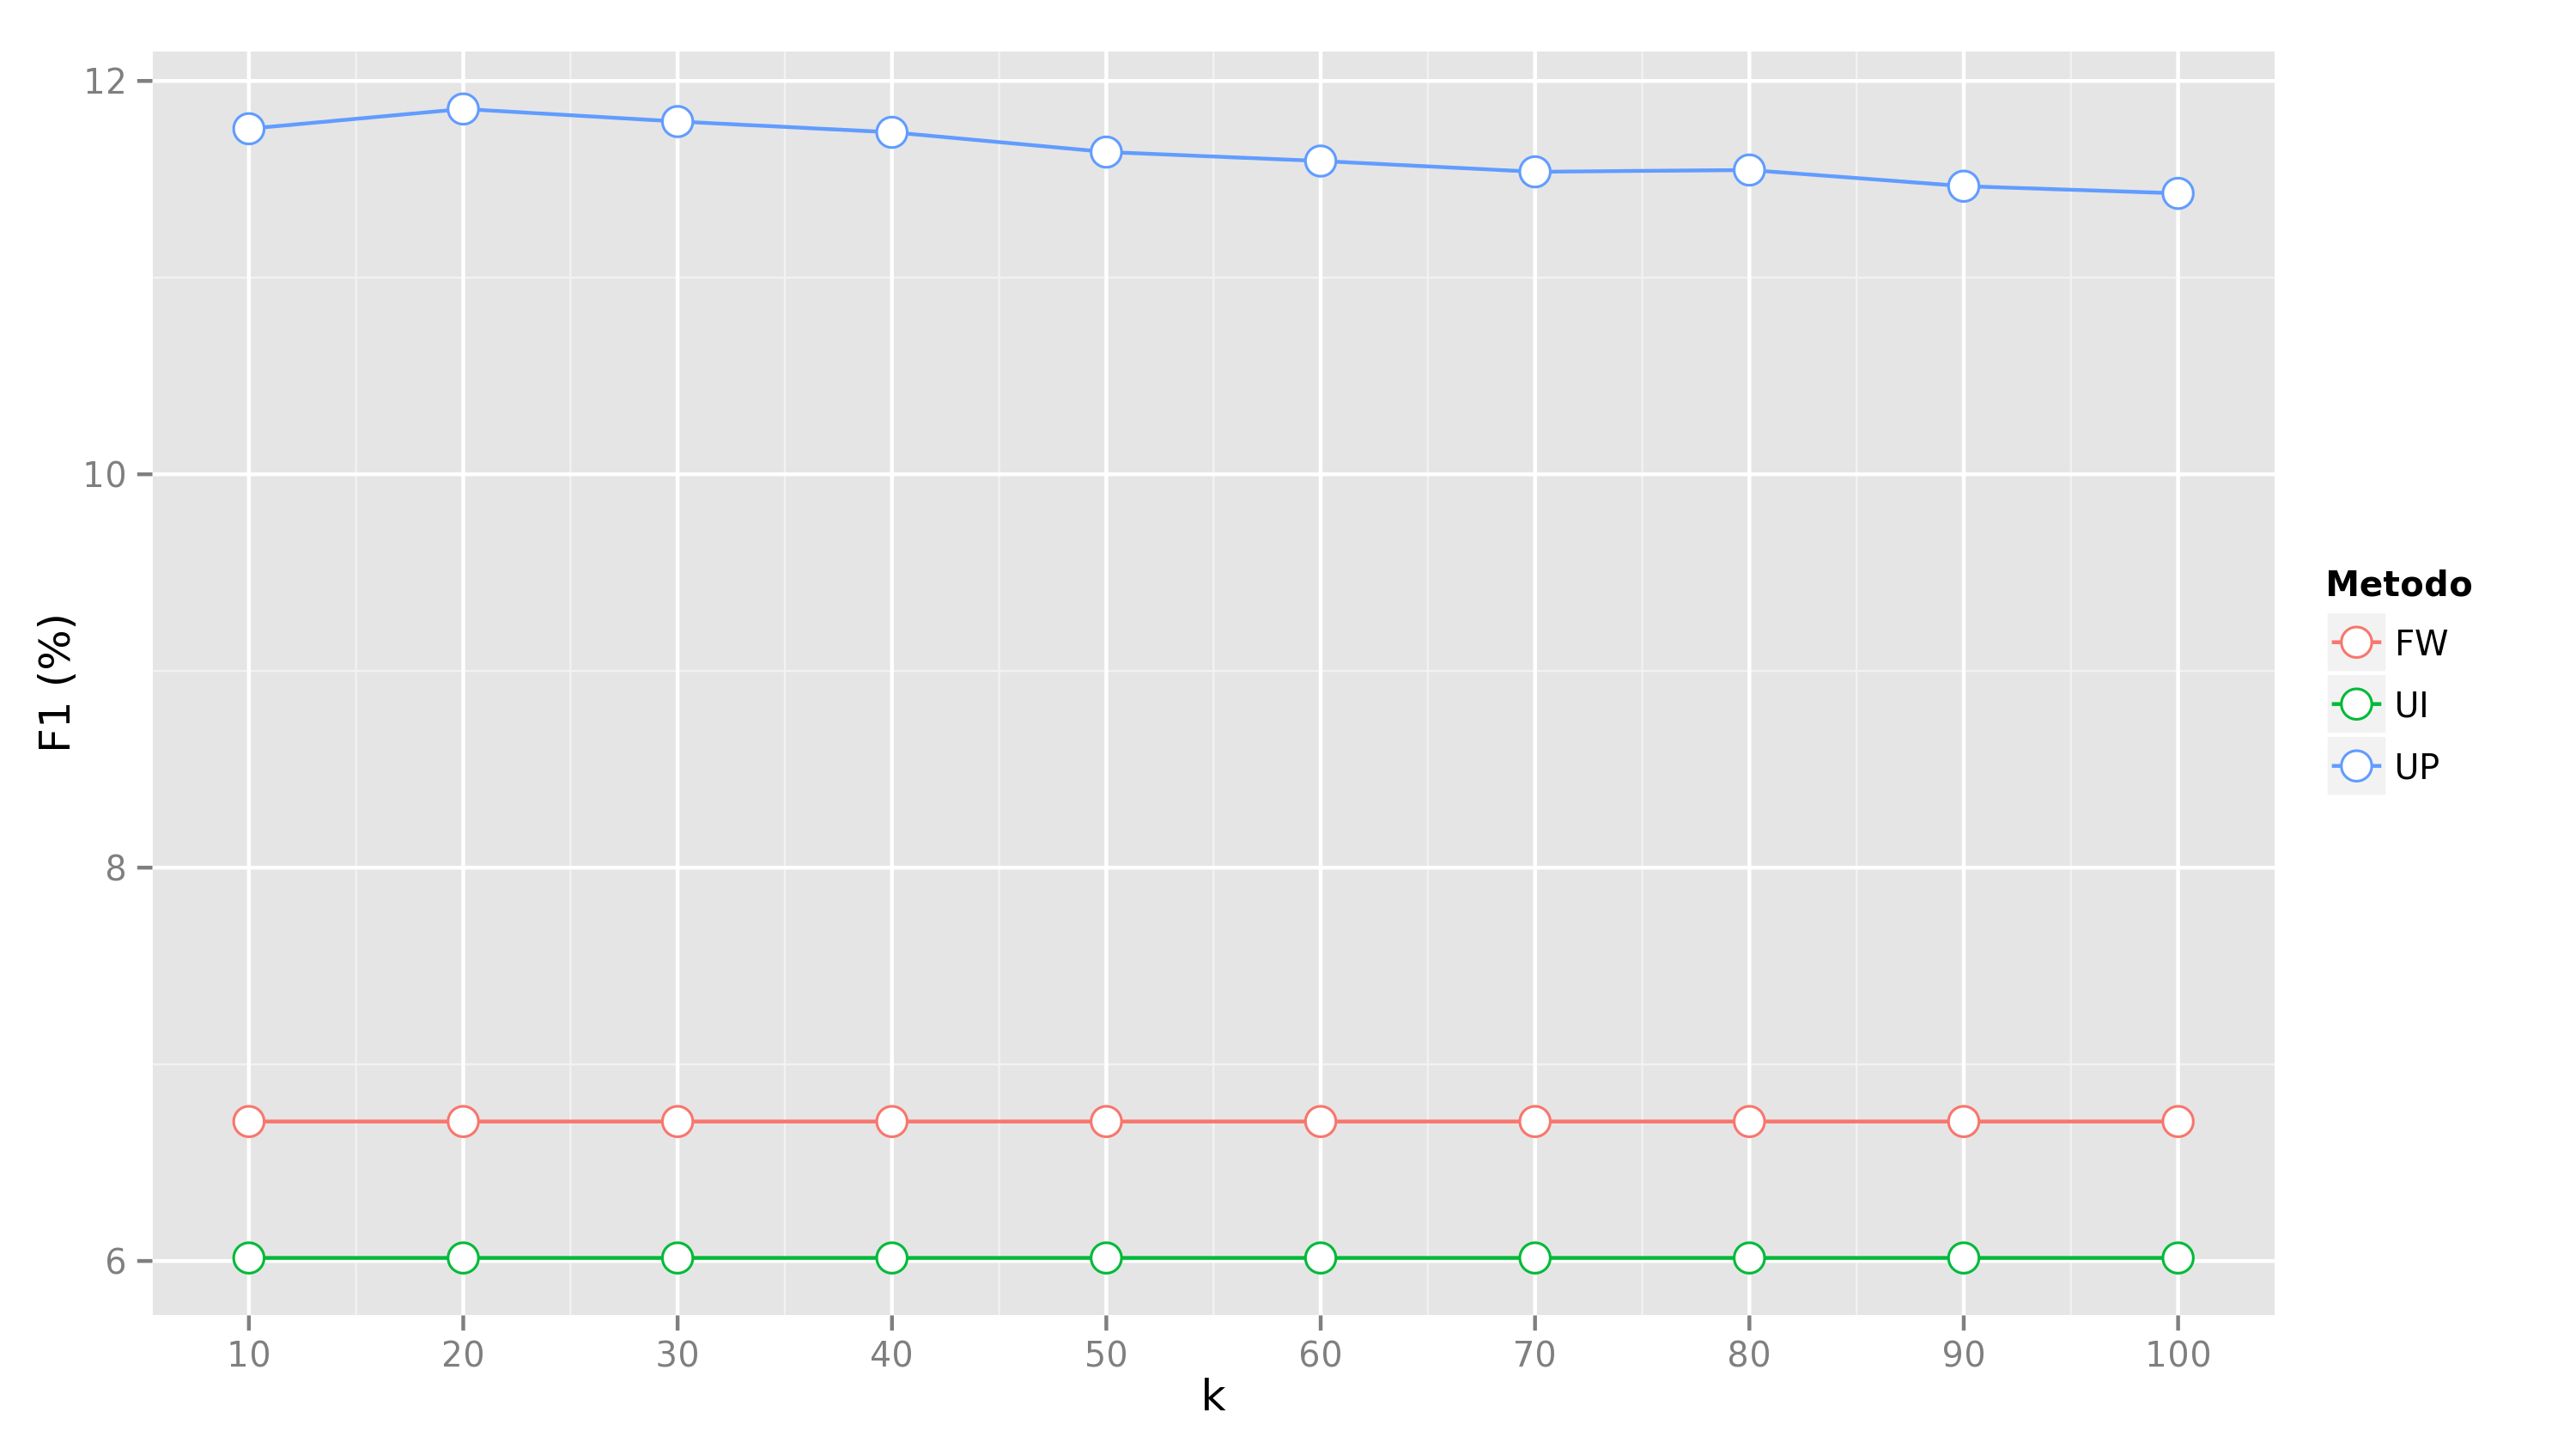
\includegraphics[width=1\textwidth]{img/F1_k}
    \end{center}
    \label{fig:F1_k}
    \caption{Medida $F_1$ em função do número de vizinhos mais próximos $k$}
\end{figure}

\begin{figure}[htp]
    \begin{center}
    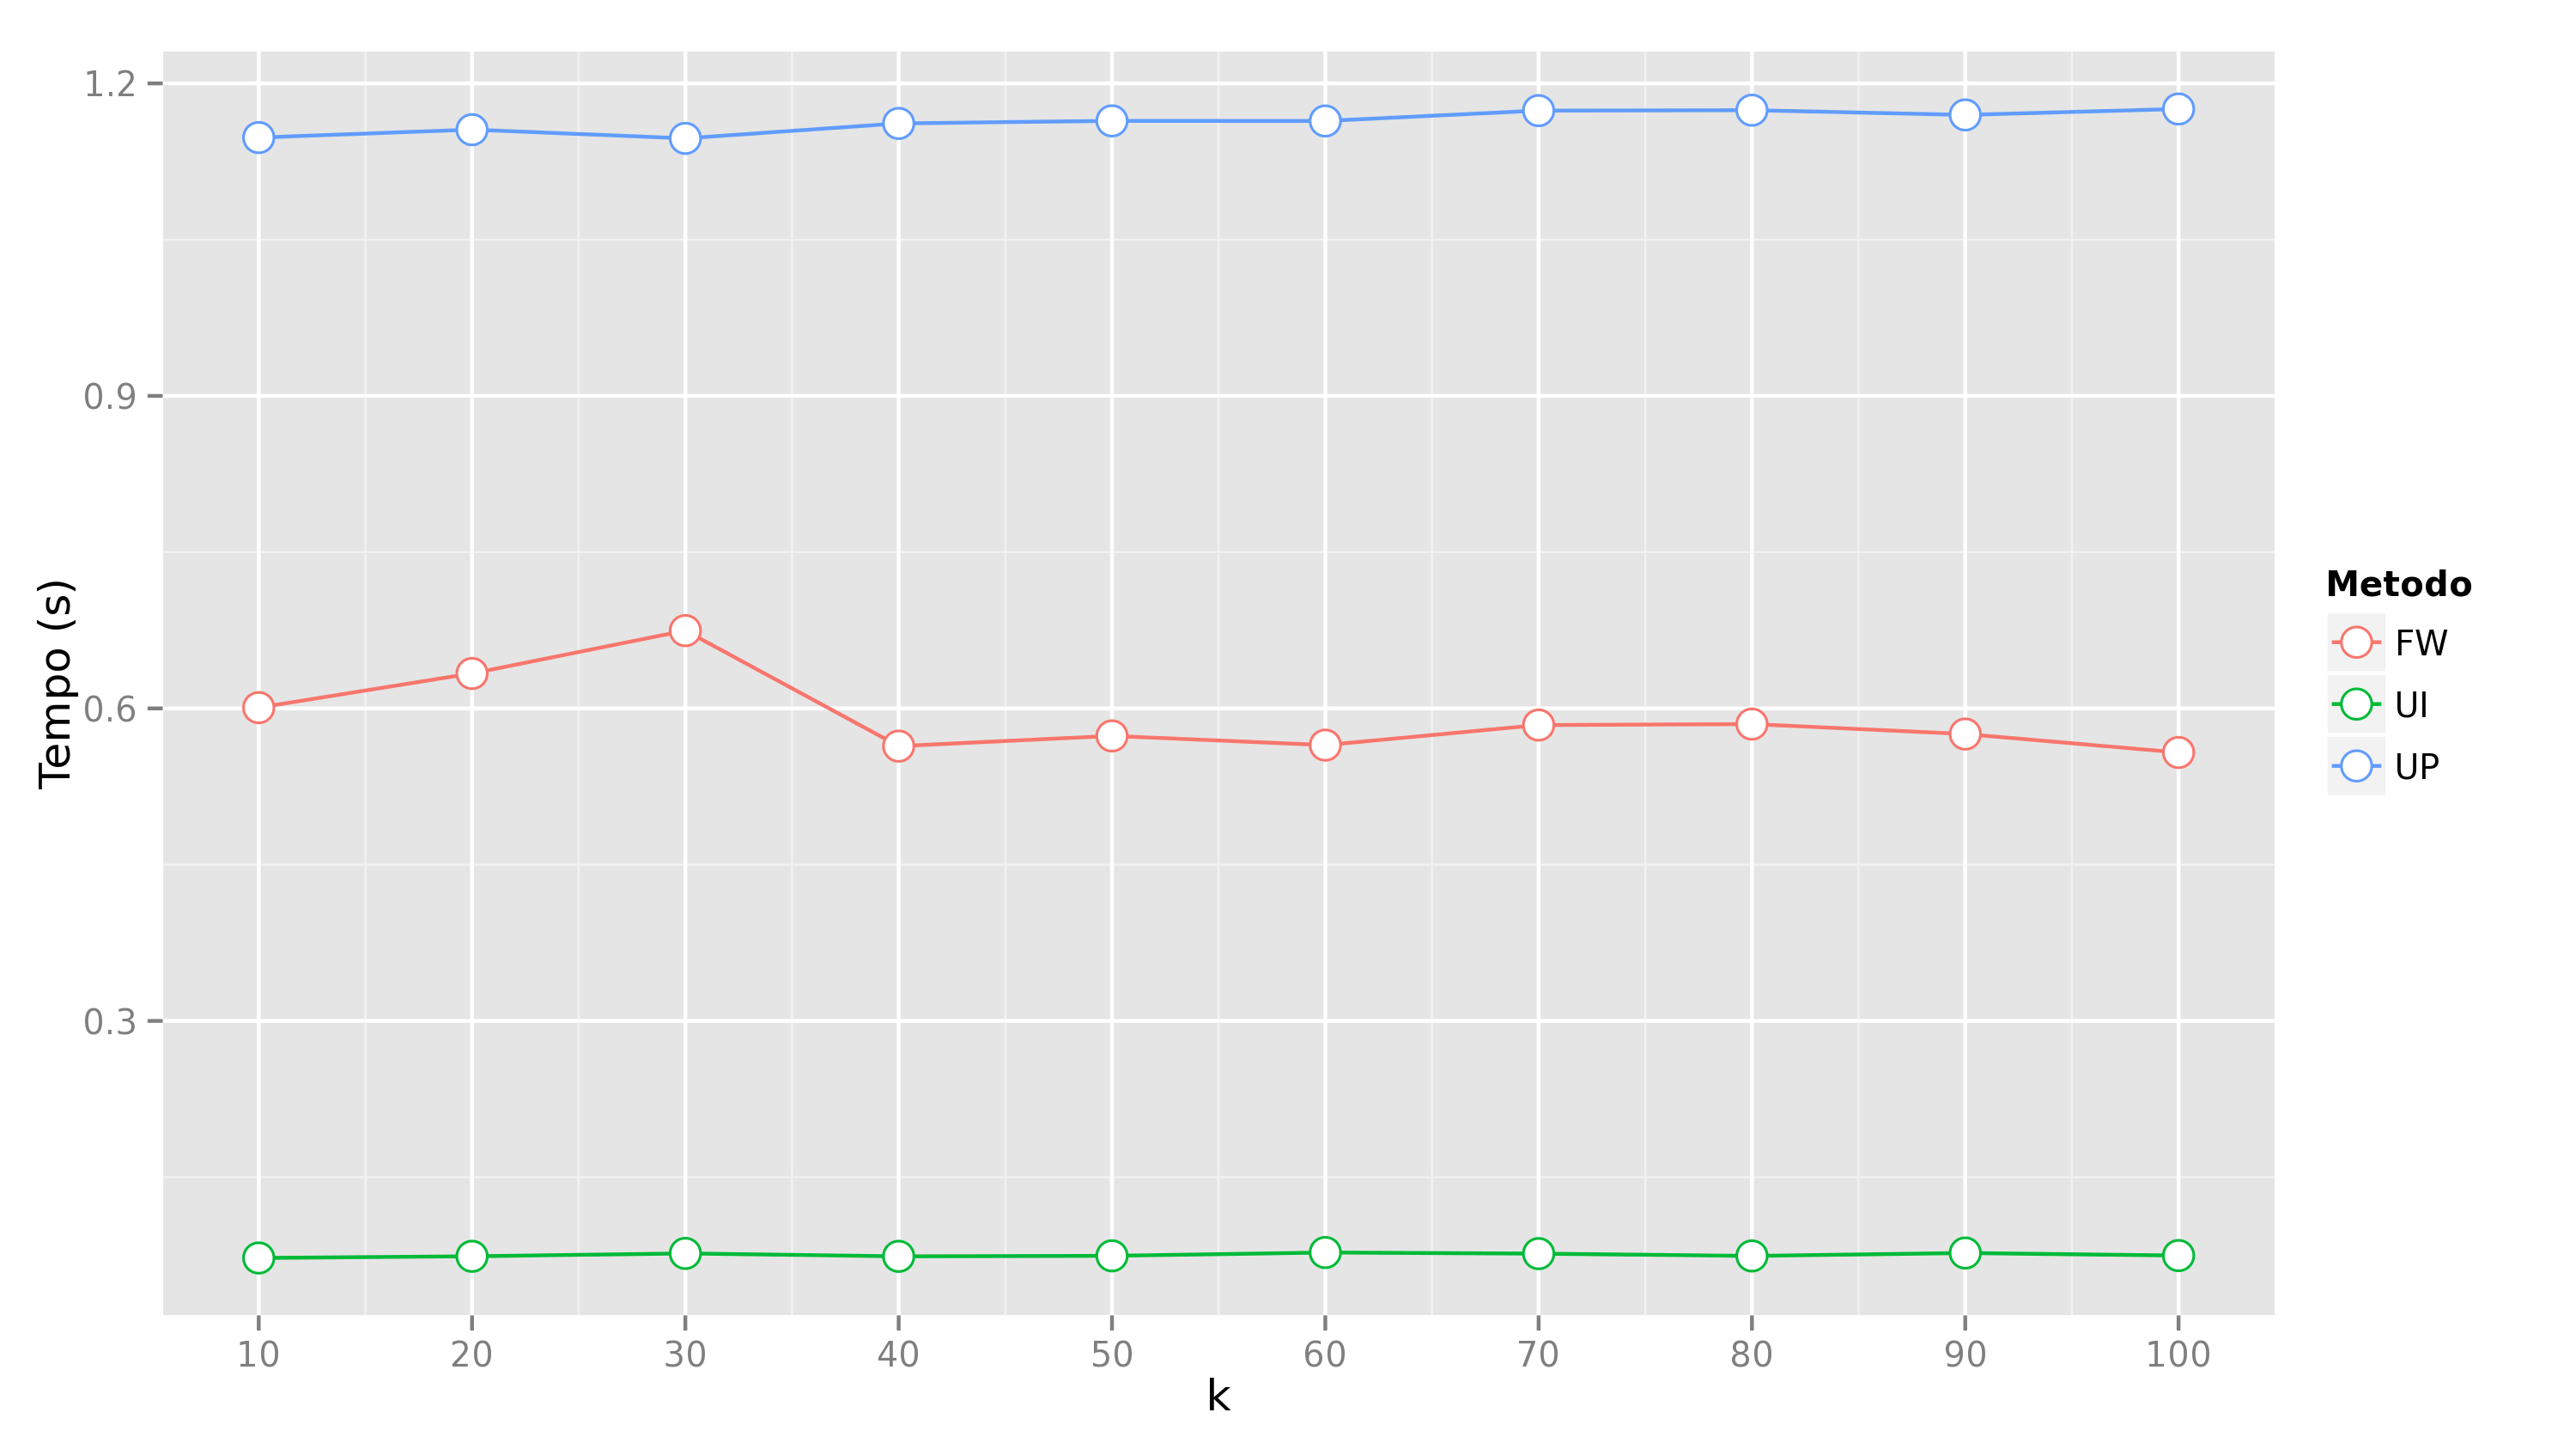
\includegraphics[width=1\textwidth]{img/time_k}
    \end{center}
    \label{fig:time_k}
    \caption{Tempo de execução em função do número de vizinhos mais próximos $k$}
\end{figure}

\section{Conjunto de atributos dos itens
 $\mathcal{F}$} % (fold)
\label{sec:conjunto_de_atributos_dos_itens_}


\section{Medida de distância entre atributos $d^f$} % (fold)
\label{sec:medida_de_dist_ncia_entre_atributos_}


\section{Pesos dos atributos $w_f$} % (fold)
\label{sec:pesos_dos_atributos_}

% section pesos_dos_atributos_ (end)

























\chapter[old]{old}
\label{chap:old}

\section{Primeira etapa do Trabalho de Conclusão de Curso} % (fold)
\label{sec:primeira_etapa_do_trabalho_de_conclus_o_de_curso}

% section primeira_etapa_do_trabalho_de_conclus_o_de_curso (end)
Os resultados da primeira etapa deste Trabalho de Conclusão de Curso, realizadas na disciplina PMR2500, foram principalmente a definição de necessidades, de parâmetros de sucesso e a elaboração de possíveis soluções. 

Definimos que a aquisição de dados seria feita a partir de uma base qualquer, que deveria alimentar o sistema por meio de arquivos de texto com valores separados por vírgulas (\texttt{.csv}).

A fim de facilitar o pré-processamento dos dados, estabelecemos que seriam necessários dois arquivos. Um deles deve conter a matriz de atributos $\mathbf{A}$ e o outro, a matriz de avaliações  $\mathbf{R}$. 

\begin{equation} 
\mathbf{A} = 
\begin{bmatrix} 
 a_{i_1 f_1} &  a_{i_1 f_2} &  a_{i_1 f_3}  & \dots   \\
 a_{i_2 f_1} &  a_{i_2 f_2} &  a_{i_2 f_3}  & \dots   \\
 a_{i_3 f_1} &  a_{i_3 f_2} &  a_{i_3 f_3}  & \dots  \\ 
 \vdots &  \vdots &  \vdots  & \ddots   \\
 \end{bmatrix}
\end{equation}


\begin{equation}
	  \mathbf{R} = 
\begin{bmatrix} 
  r_{u_1 i_1} &  r_{u_1 i_2} &  r_{u_1 i_3}  & \dots   \\
 r_{u_2 i_1} &  r_{u_2 i_2} &  r_{u_2 i_3}  & \dots   \\
 r_{u_3 i_1} &  r_{u_3 i_2} &  r_{u_3 i_3}  & \dots  \\ 
 \vdots &  \vdots &  \vdots  & \ddots   \\
\end{bmatrix}
\end{equation}

Em alguns bancos de dados relacionais, a tabela de avaliações também contém informações adicionais $\theta$, tais como método de pagamento, data da compra, data de entrega, etc., e é denominada matriz histórico de avaliações $\mathbf{H}$. Optamos, no nosso projeto, por não aceitar esse tipo de informação, e nem tampouco dados ligados a características de clientes (matriz $\mathbf{B}$). Para o emprego do sistema de recomendação em um e-commerce real, deve-se portanto efetuar ajustes no algoritmo a fim de tratar de particularidades envolvendo informações adicionais e arquivos suplementares.

\begin{equation} 
\mathbf{H} =
\begin{bmatrix} 
 r_{u_1 i_1} &  \theta_{h_1 1} &  \theta_{h_1 2} & \dots   \\
 r_{u_1 i_2} &  \theta_{h_2 1} &  \theta_{h_2 2} & \dots   \\
 r_{u i} &  \theta_{h 1} &  \theta_{h 2} & \dots   \\
 \vdots &  \vdots &  \vdots  & \ddots   \\
 \end{bmatrix} \\
\end{equation}

\begin{equation}
	\mathbf{B} = 
\begin{bmatrix} 
 b_{u_1 c_1} &  b_{u_1 c_2} &  b_{u_1 c_3}  & \dots   \\
 b_{u_2 c_1} &  b_{u_2 c_2} &  b_{u_2 c_3}  & \dots   \\
 b_{u_3 c_1} &  b_{u_3 c_2} &  b_{u_3 c_3}  & \dots  \\ 
 \vdots &  \vdots &  \vdots  & \ddots   \\
 \end{bmatrix}
\end{equation}

Uma vez determinada a forma de entrada de informações, definiram-se os conjuntos de dados que serão utilizados. O primeiro conjunto de dados abertos é proveniente do sistema de recomendações de filmes MovieLens (\url{http://movielens.umn.edu}). Nessa base de dados, o catálogo de filme faz o papel de catálogo de produtos, e o histórico de compras se refere à avaliação dos filmes feita por cada usuário. Outro conjunto de dados abertos é do website Internet Movie Database (IMDB). Na nossa análise, esses dois bancos poderão ser utilizado complementar ou independentemente.

Na primeira etapa do projeto, buscamos parcerias com e-commerces que estivessem dispostos a doar anonimamente seu banco de dados. Há ainda a possibilidade de utilizarmos uma terceira base, mas visto que as negociações ainda não foram concluídas, daremos prioridades aos conjuntos \textit{open source}.  

\section{Segunda etapa do Trabalho de Conclusão de Curso} % (fold)
\label{sec:segunda_etapa_do_trabalho_de_conclus_o_de_curso}

% section segunda_etapa_do_trabalho_de_conclus_o_de_curso (end)

A partir da síntese de soluções estabelecida na primeira etapa do projeto, implementamos os três algoritmos de recomendação e as medidas de recomendação na linguagem de programação estatística R. O código já está disponível para consulta através do endereço \url{https://github.com/aviggiano/tcc}.

Ainda na etapa de implementação, confirmamos a validade de cada um dos métodos aplicando-os nas matrizes-referência (Tabelas \ref{tab:rui_ref} e \ref{tab:aif_ref}). 

Em seguida, fizemos o tratamento das bases de dados, adequando-as ao formato de entrada especificado, e  iniciamos o processo de desenvolvimento do \textit{cross-validation}.

Para os trabalhos futuros, iremos realizar a validação cruzada e avaliar se os requisitos funcionais foram estabelecidos. Em seguida, procuraremos melhorar o sistema de recomendação a fim de torná-lo mais genérico. Buscaremos eliminar restrições quanto a entrada e saída de dados, de forma que elas sejam completamente arbitrárias. O objetivo é que o usuário possa informar ao sistema como é formado sua base, e que todo o tratamento preliminar seja feito automaticamente. 

Caso haja tempo, trabalharemos também na construção de um \textit{driver} que possibilite a conexão entre o sistema de recomendação e um banco de dados SQL, sem que seja necessária a etapa intermediária de arquivos \texttt{csv} para aquisição de dados. Planejamos elaborar um \textit{website} para o sistema de recomendação e exportar toda a lógica para um servidor dedicado. Outra melhoria desejada é a reconstrução dos métodos na linguagem de programação C, a fim de melhorar a performance computacional. Dessa forma, o serviço de ``sistema de recomendação nas nuvens'' estaria completo e poderia ser utilizado por e-commerces reais.